\chapter{Quench Localization Problem (\qlp)}
\label{chp:qlp}
This chapter is dedicated to the resolution of the Quench Localization Problem, as we did for \qrp,
we will discuss:
\begin{inparaenum}[(i)]
	\item some of the preprocessing we have done, specific for the labels,
	\item the first approaches with clustering, and finally,
	\item the results obtained, just like we did in \Cref{sec:results-qrp}
\end{inparaenum}.
\section{Problem description}
\section{Data preprocessing}
\label{sec:qlp-preprocessing}
Since the essential difference between the dataset used for \qlp\ and the dataset used for \qrp\,
are the labels, in this section we will concentrate on the considerations arisen from the analysis
of the new labels and the distribution of the points in a bidimensional space. Once more, we will be
splitting the section in different subsections, one for each attribute in the dataset.

\subsubsection{\an}
The correlation with the labels has been plotted in \Cref{fig:an-lcorr-qlp}, as we can see, \an is
correlated very strongly with coils $0$ and $2$, while the correlation is basically non-existent in the
case of coils $1$ and $3$. If we remind ourselves of the correlation existing among the harmonics,
shown in \Cref{fig:an-corr}, we can see that:
\begin{itemize}
	\item Contrarily to what we discovered in \Cref{sec:qrp-preprocessing}, the correlation
	      between harmonic number $2$ and the solution is not strong anymore (for none of the
	      coils);
	\item Now we have a strong correlation for harmonics number $1$ and $3$ (which are very
	      strongly correlated with each other, see \Cref{fig:an-corr}, therefore we will not be able
	      to use them together);
\end{itemize}
A potential dataset could be constructed using a primary odd harmonic (like $1$ or $3$), the
harmonic performing the best among $4, 8$ and $12$ (which are all strongly correlated, see
\Cref{fig:an-corr}) and finally another harmonic between the ones that have been left out. Due to
the very low correlation between the \an\ and the labels for coil $1$ and $3$ we didn't really
consider it as an attribute worth exploring.

\begin{figure}[!h]
	% Font size = 70
	\centering
	\begin{subfigure}{0.49\linewidth}
		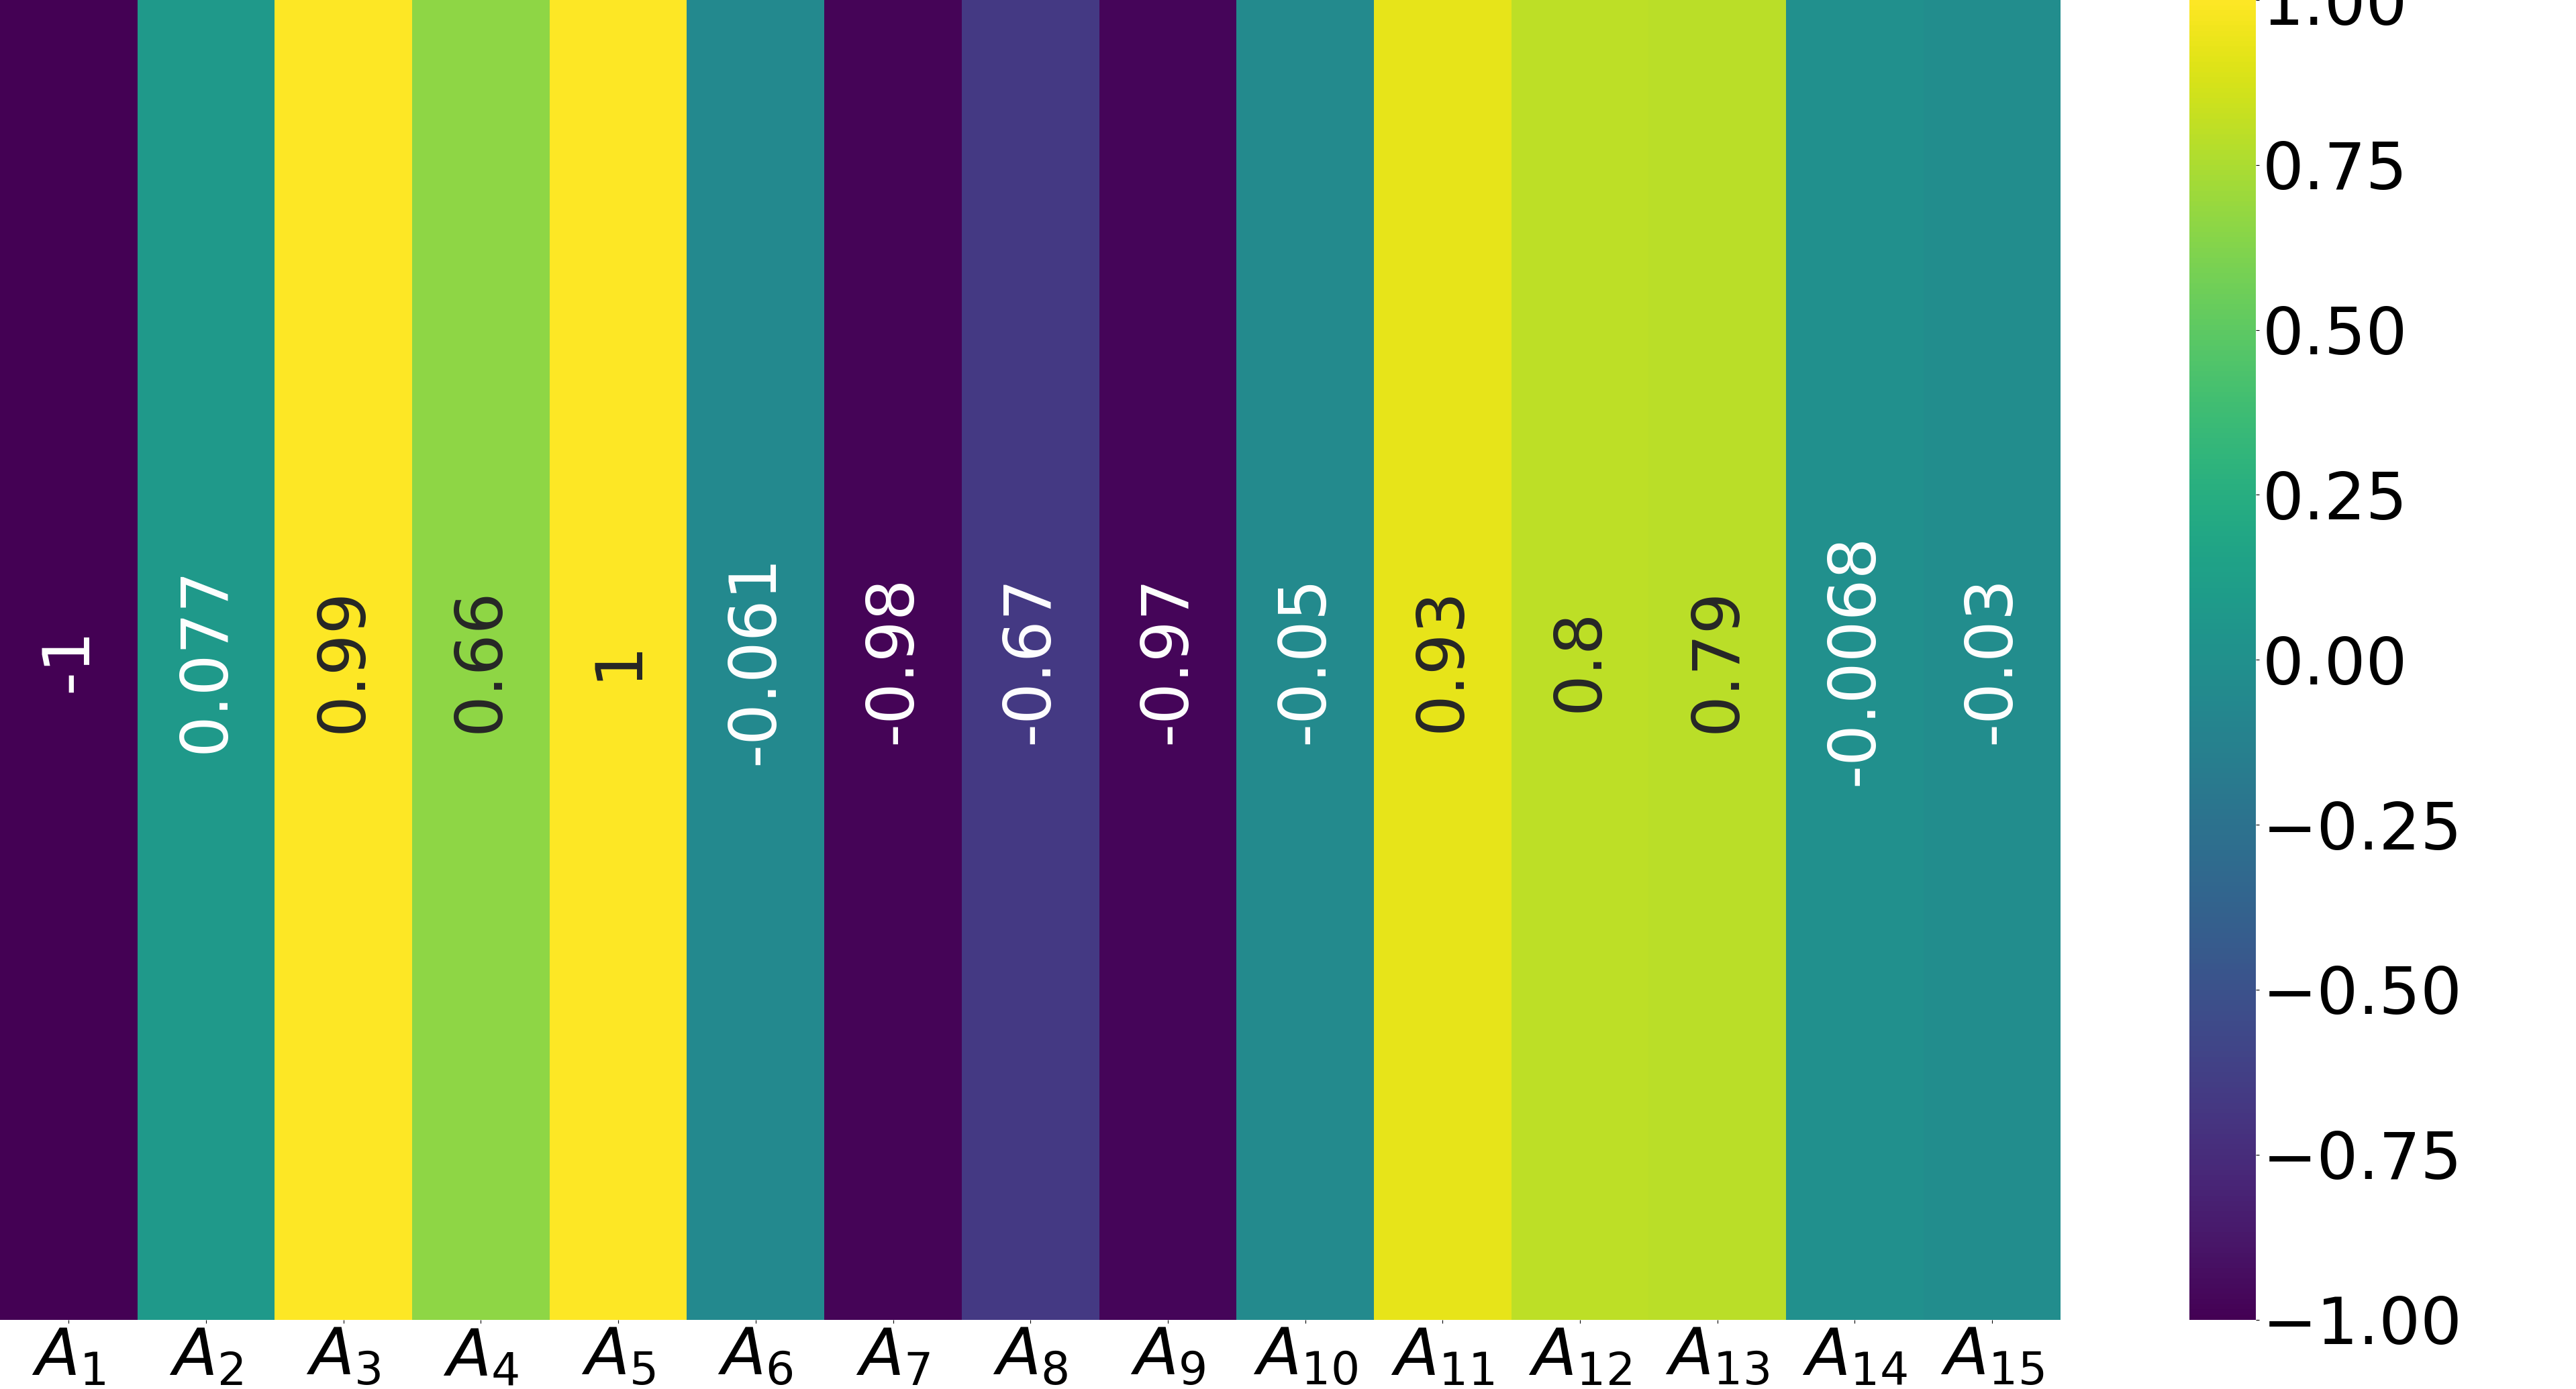
\includegraphics[width=\linewidth]{img/qlp_corr/An_coil0.png}
		\subcaption{Correlation with coil $0$}
	\end{subfigure}
	\begin{subfigure}{0.49\linewidth}
		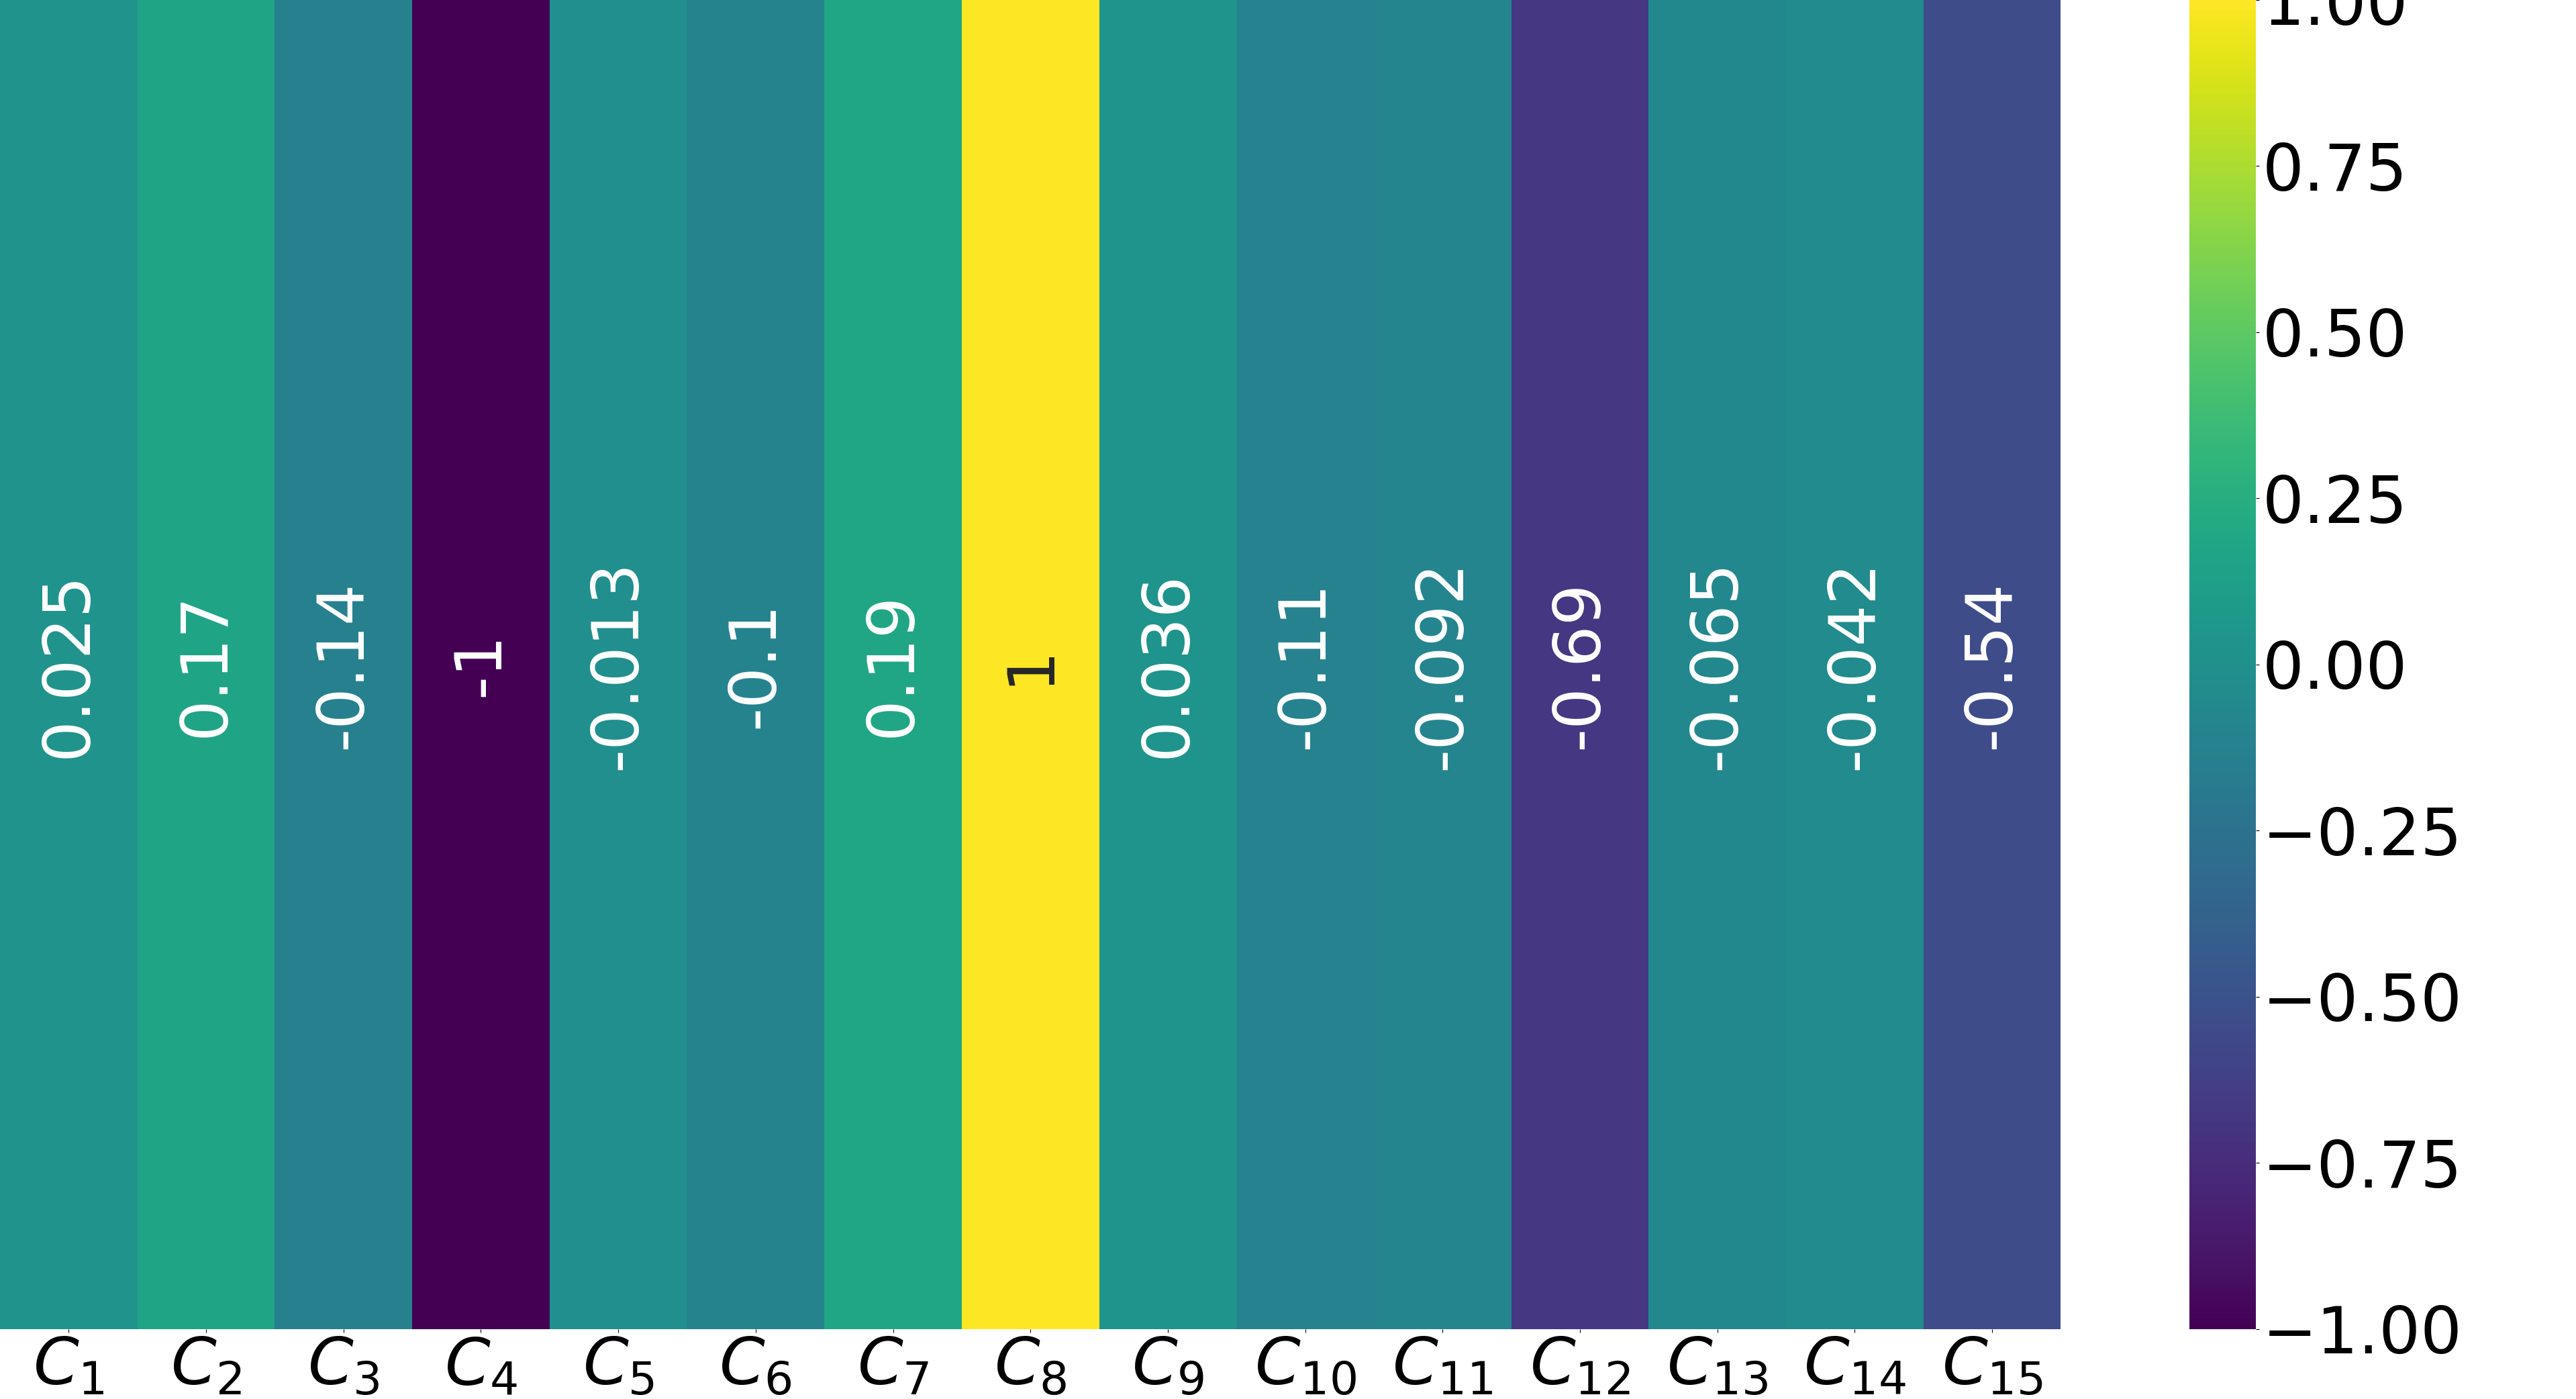
\includegraphics[width=\linewidth]{img/qlp_corr/An_coil1.png}
		\subcaption{Correlation with coil $1$}
	\end{subfigure}
	\begin{subfigure}{0.49\linewidth}
		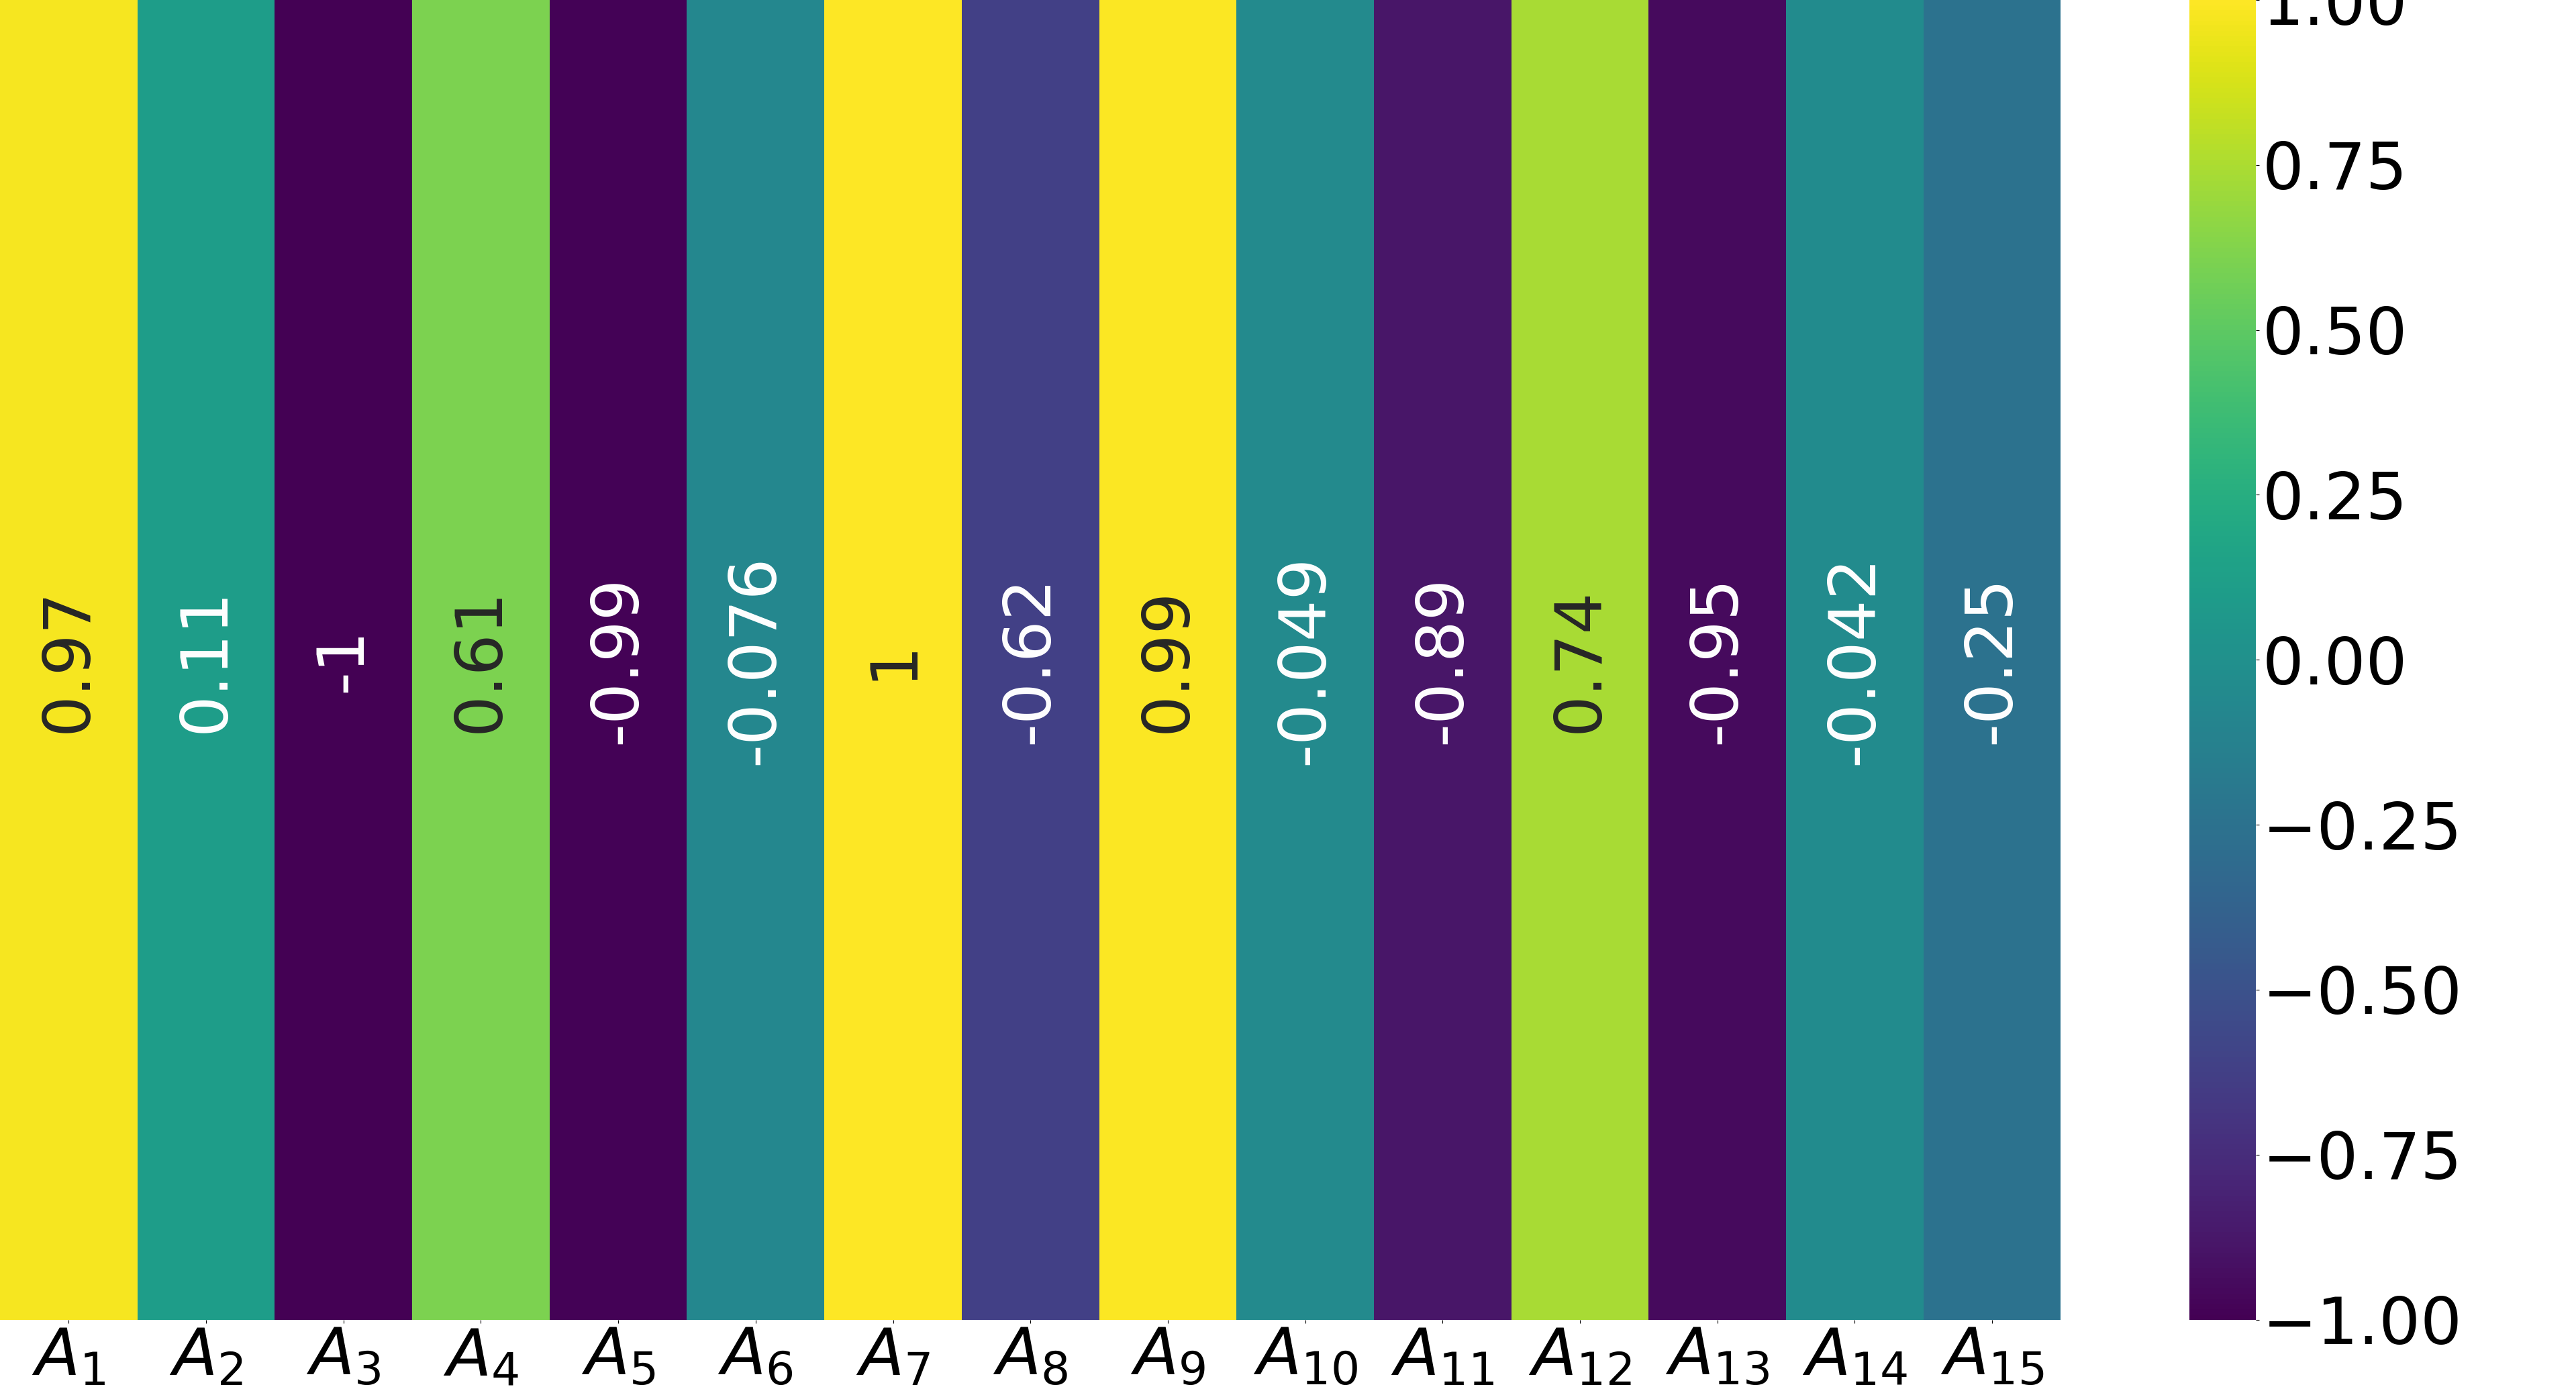
\includegraphics[width=\linewidth]{img/qlp_corr/An_coil2.png}
		\subcaption{Correlation with coil $2$}
	\end{subfigure}
	\begin{subfigure}{0.49\linewidth}
		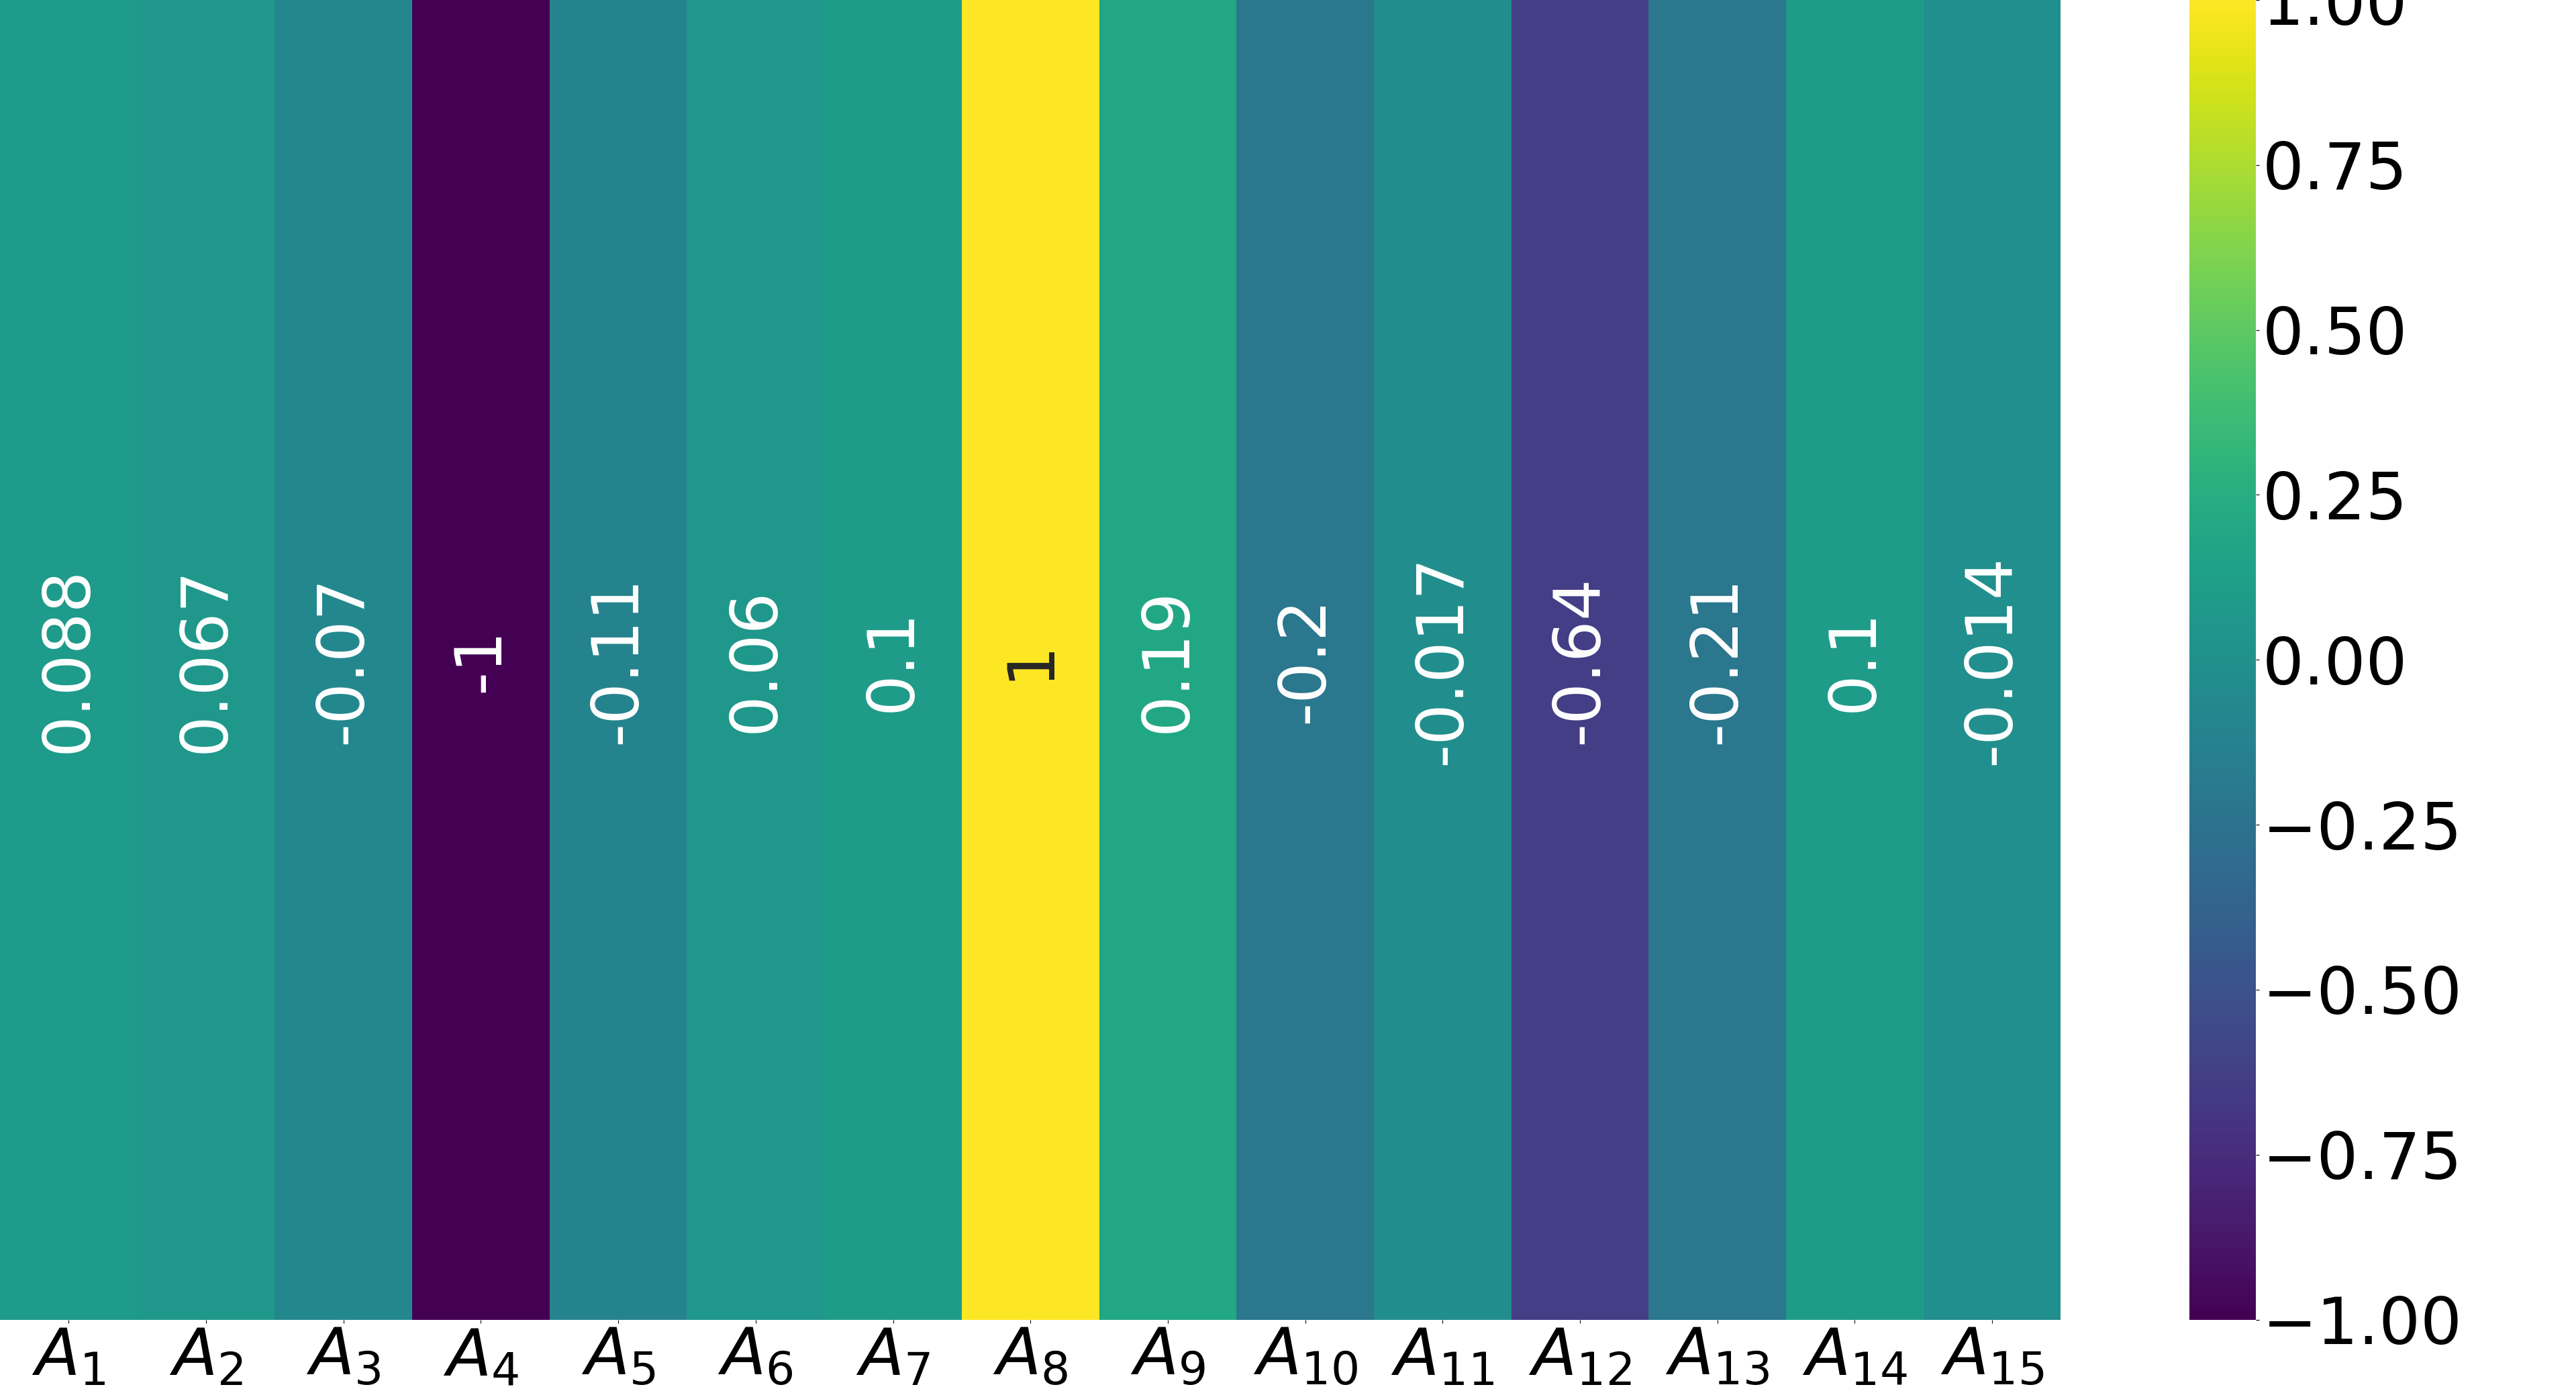
\includegraphics[width=\linewidth]{img/qlp_corr/An_coil3.png}
		\subcaption{Correlation with coil $3$}
	\end{subfigure}
	\caption{Correlation between the harmonics of the \an\ attribute and the labels for \qlp.}
	\label{fig:an-lcorr-qlp}
\end{figure}

We then used all of the infromation contained in the labels to do distribution plots, similar to the
ones we used in \Cref{chp:qrp}, to understand how data associated with single and multiple
quench-events is distributed in a bidimensional space after a round of \pca\ dimensionality
reduction. As we can see in \Cref{fig:an-coilq-dist}, the distribution of the data when working with
non-quench and single or multiple quench events (subfigure (a)) is very good, and we can easily
identify and label clusters with a high level of purity. If we consider the distribution of
quench events for single coils instead we can see that, while coil $0$ (subfigure b) and $1$ have a
fairly decent distribution, coils $1$ (subfigure c) and $3$ (subfigure e) are characterized by a
portion of the central cluster, containing in equal measure samples labelled as quench and samples
labelled as non-quench.

A less-than-ideal distribution of the samples in bidimensional space was expected due to the poor
correlation between the attribute and the labels for coils $1$ and $3$ highlighted in \Cref{fig:an-lcorr-qlp}.

\begin{figure}[!h]
	% Font size = 70
	\centering
	\begin{subfigure}{\linewidth}
		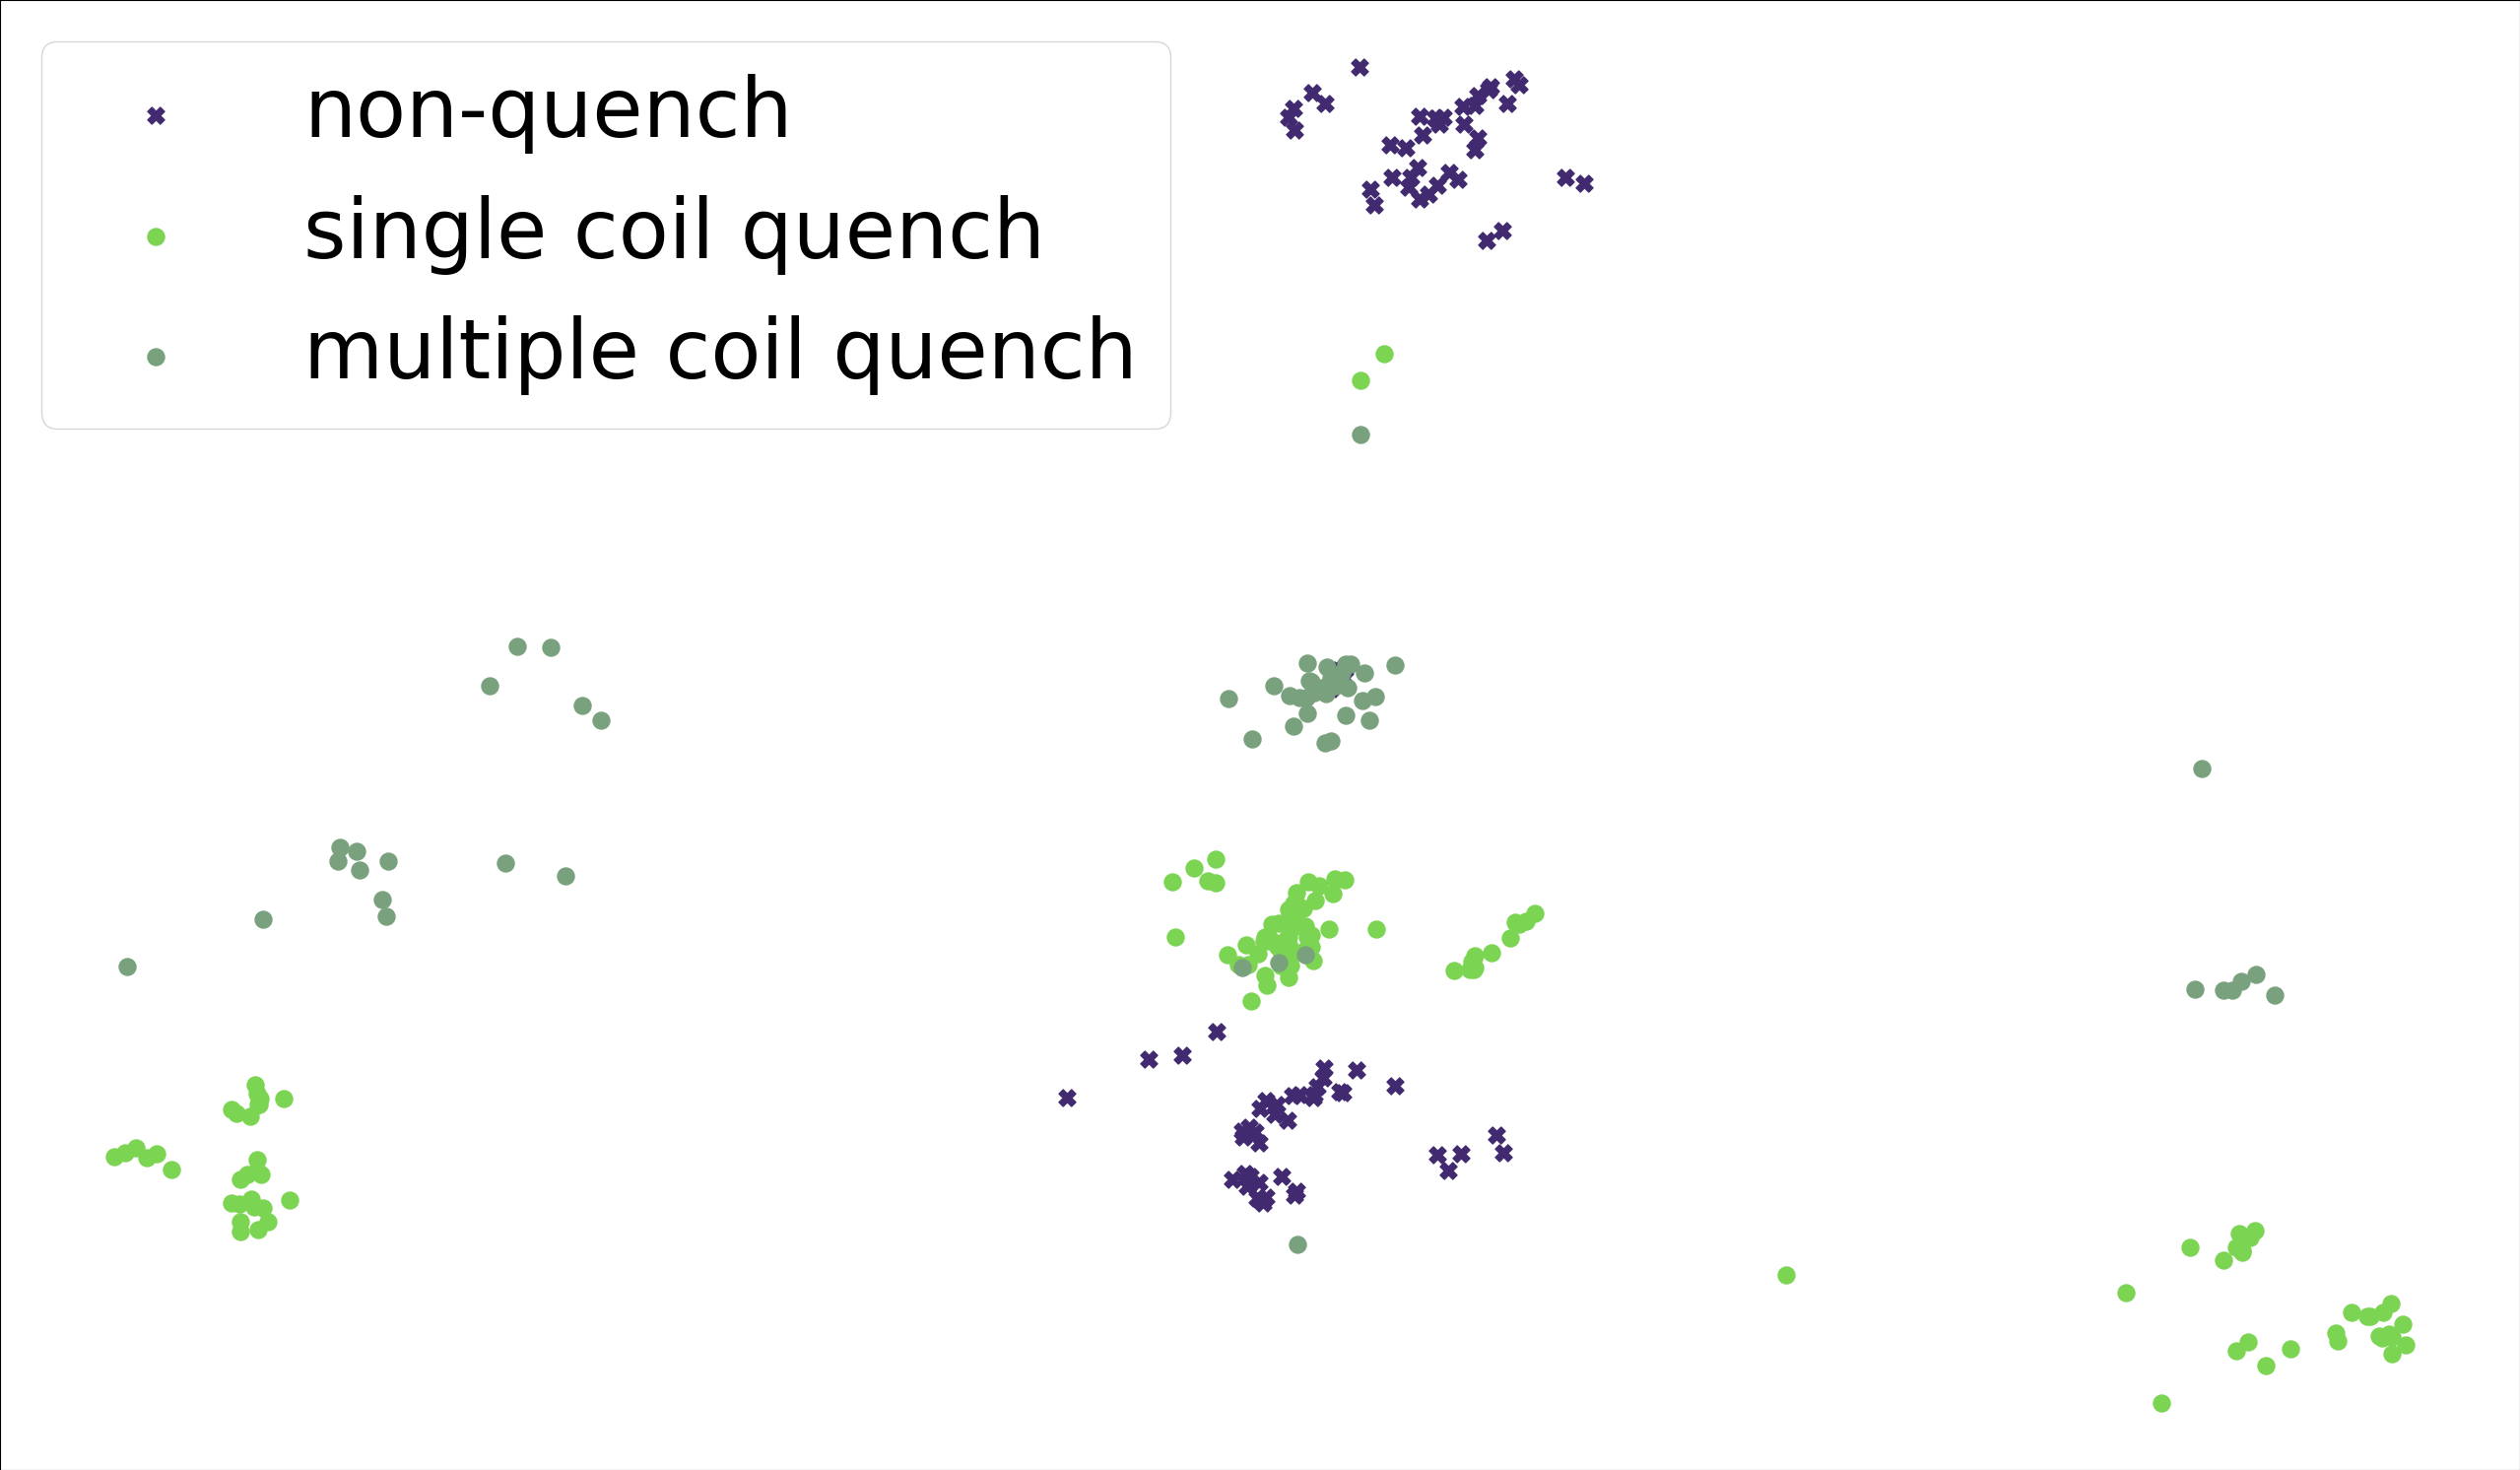
\includegraphics[width=\linewidth]{img/quench_dist_qlp/single_vs_multiple_An.png}
		\subcaption{}
	\end{subfigure}
	\begin{subfigure}{0.49\linewidth}
		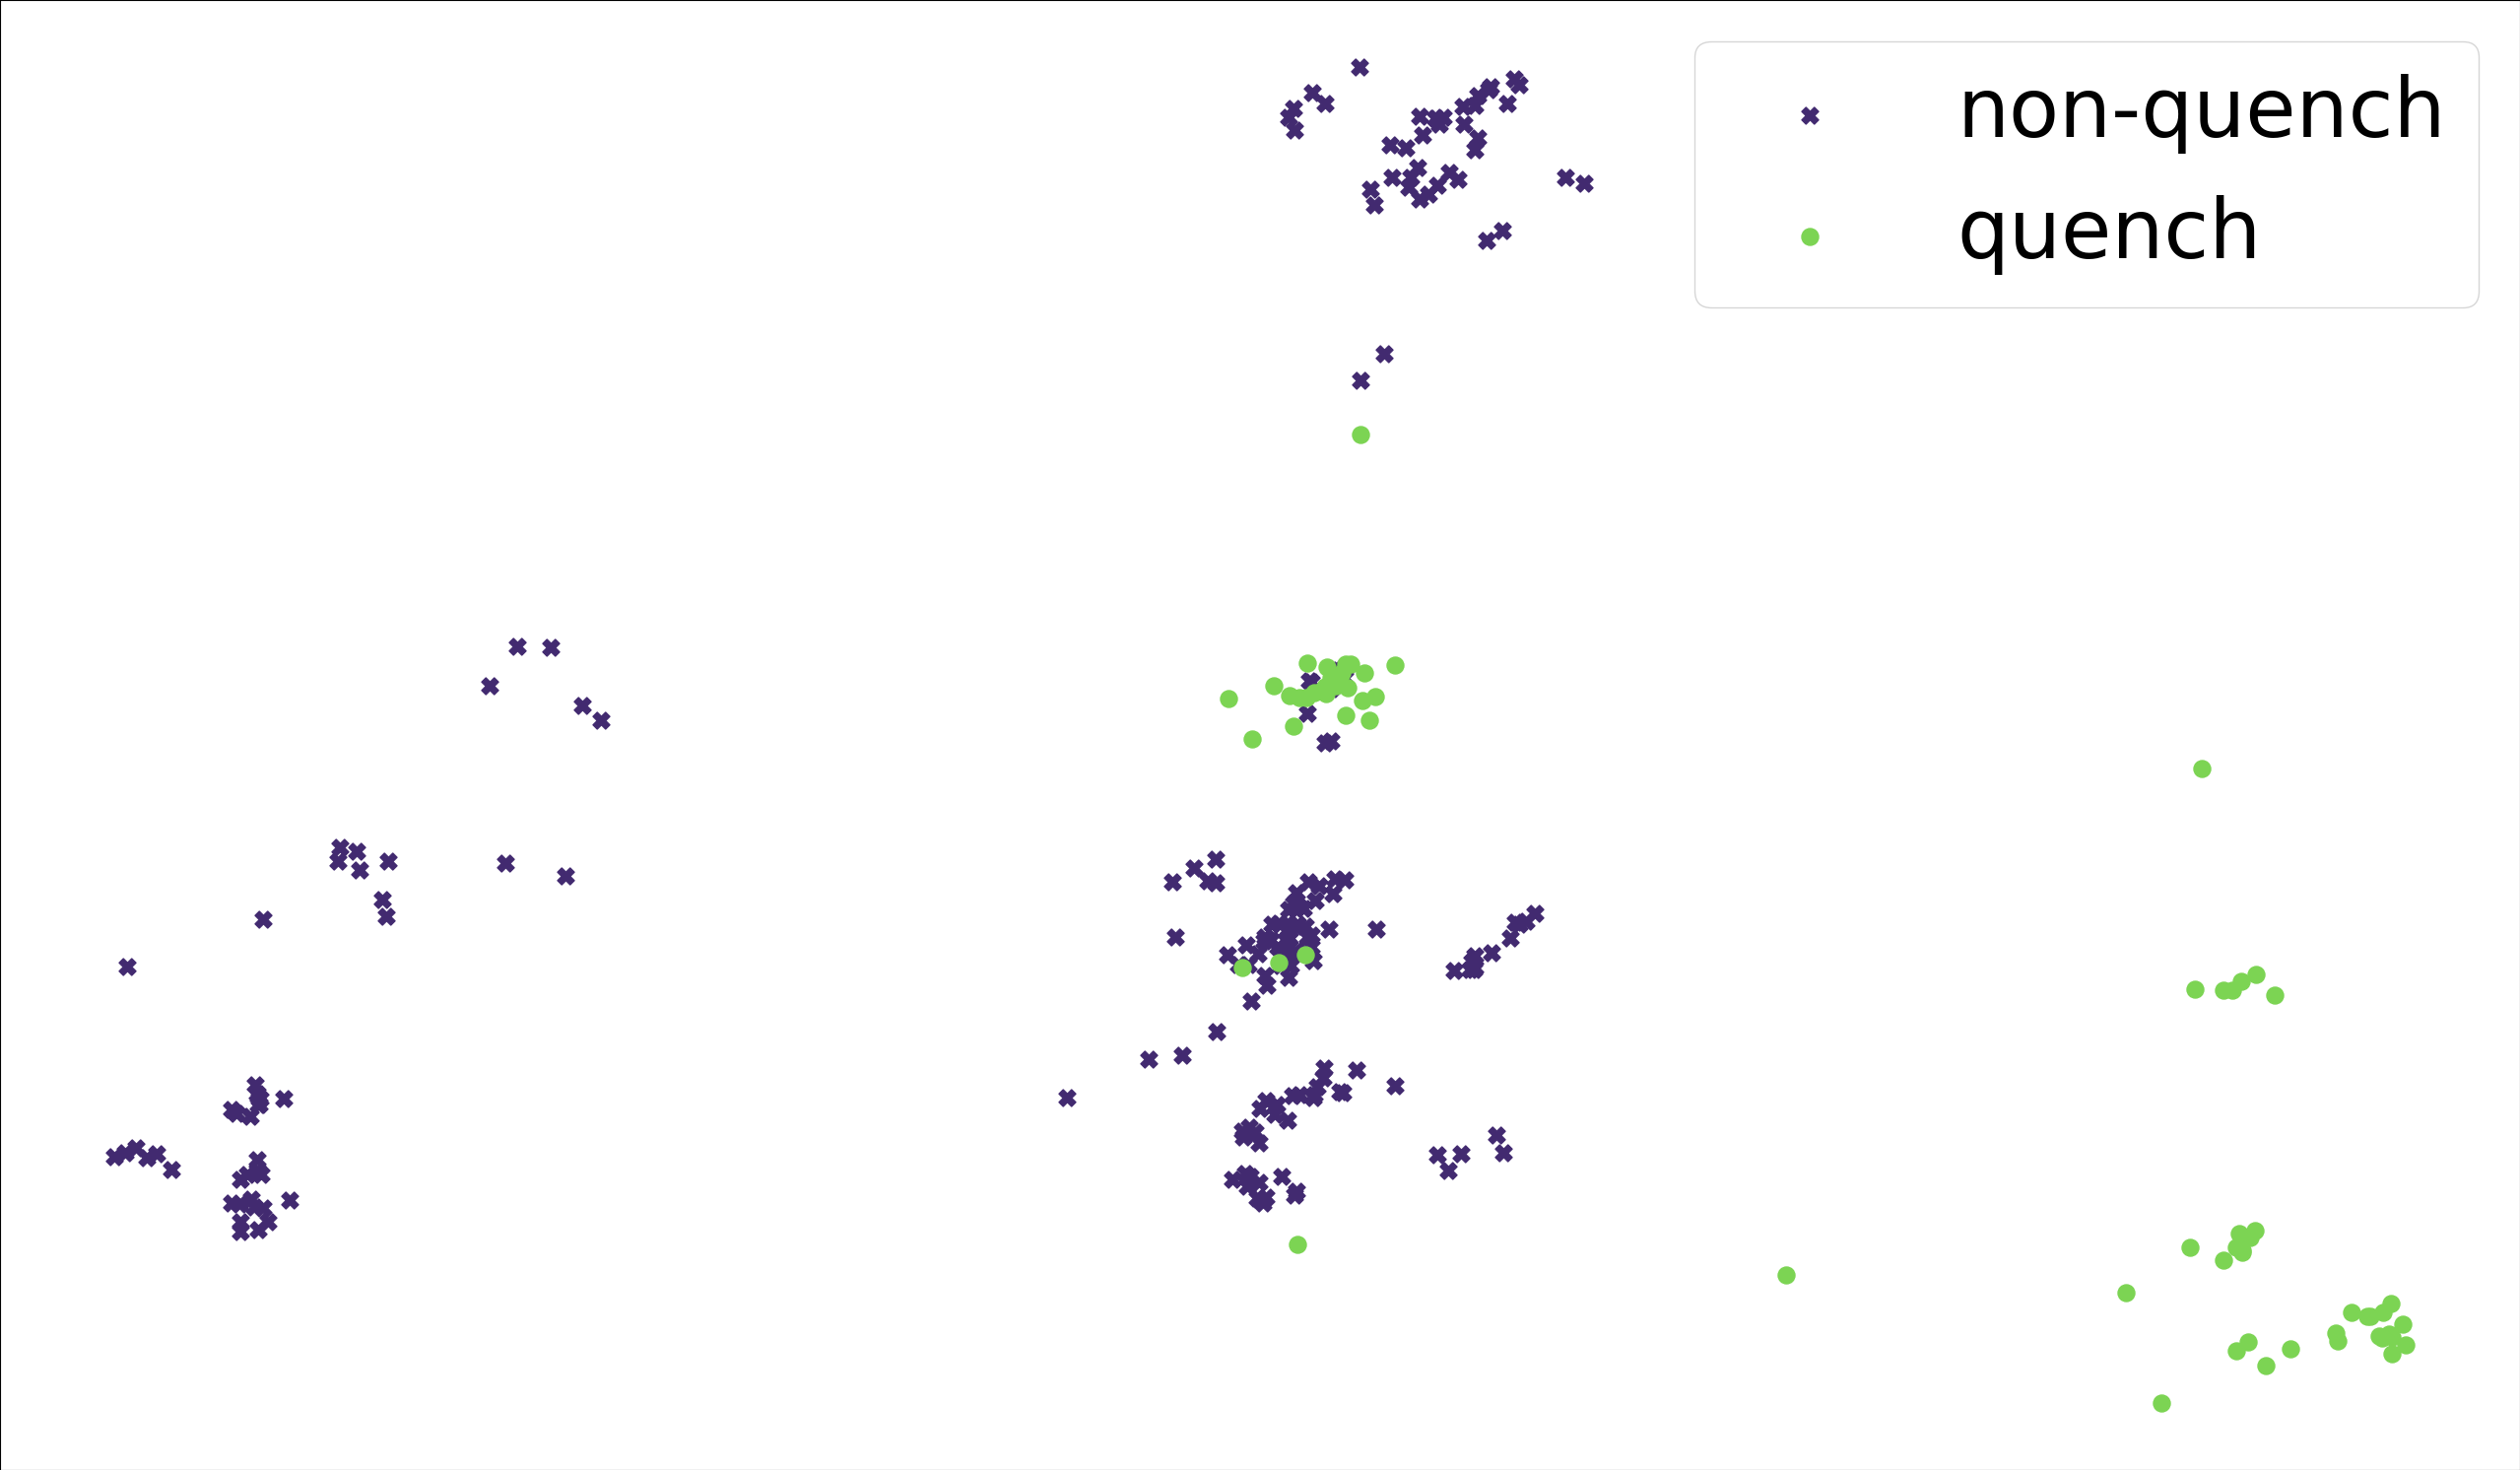
\includegraphics[width=\linewidth]{img/quench_dist_qlp/quenches_coil_0_An.png}
		\subcaption{}
	\end{subfigure}
	\begin{subfigure}{0.49\linewidth}
		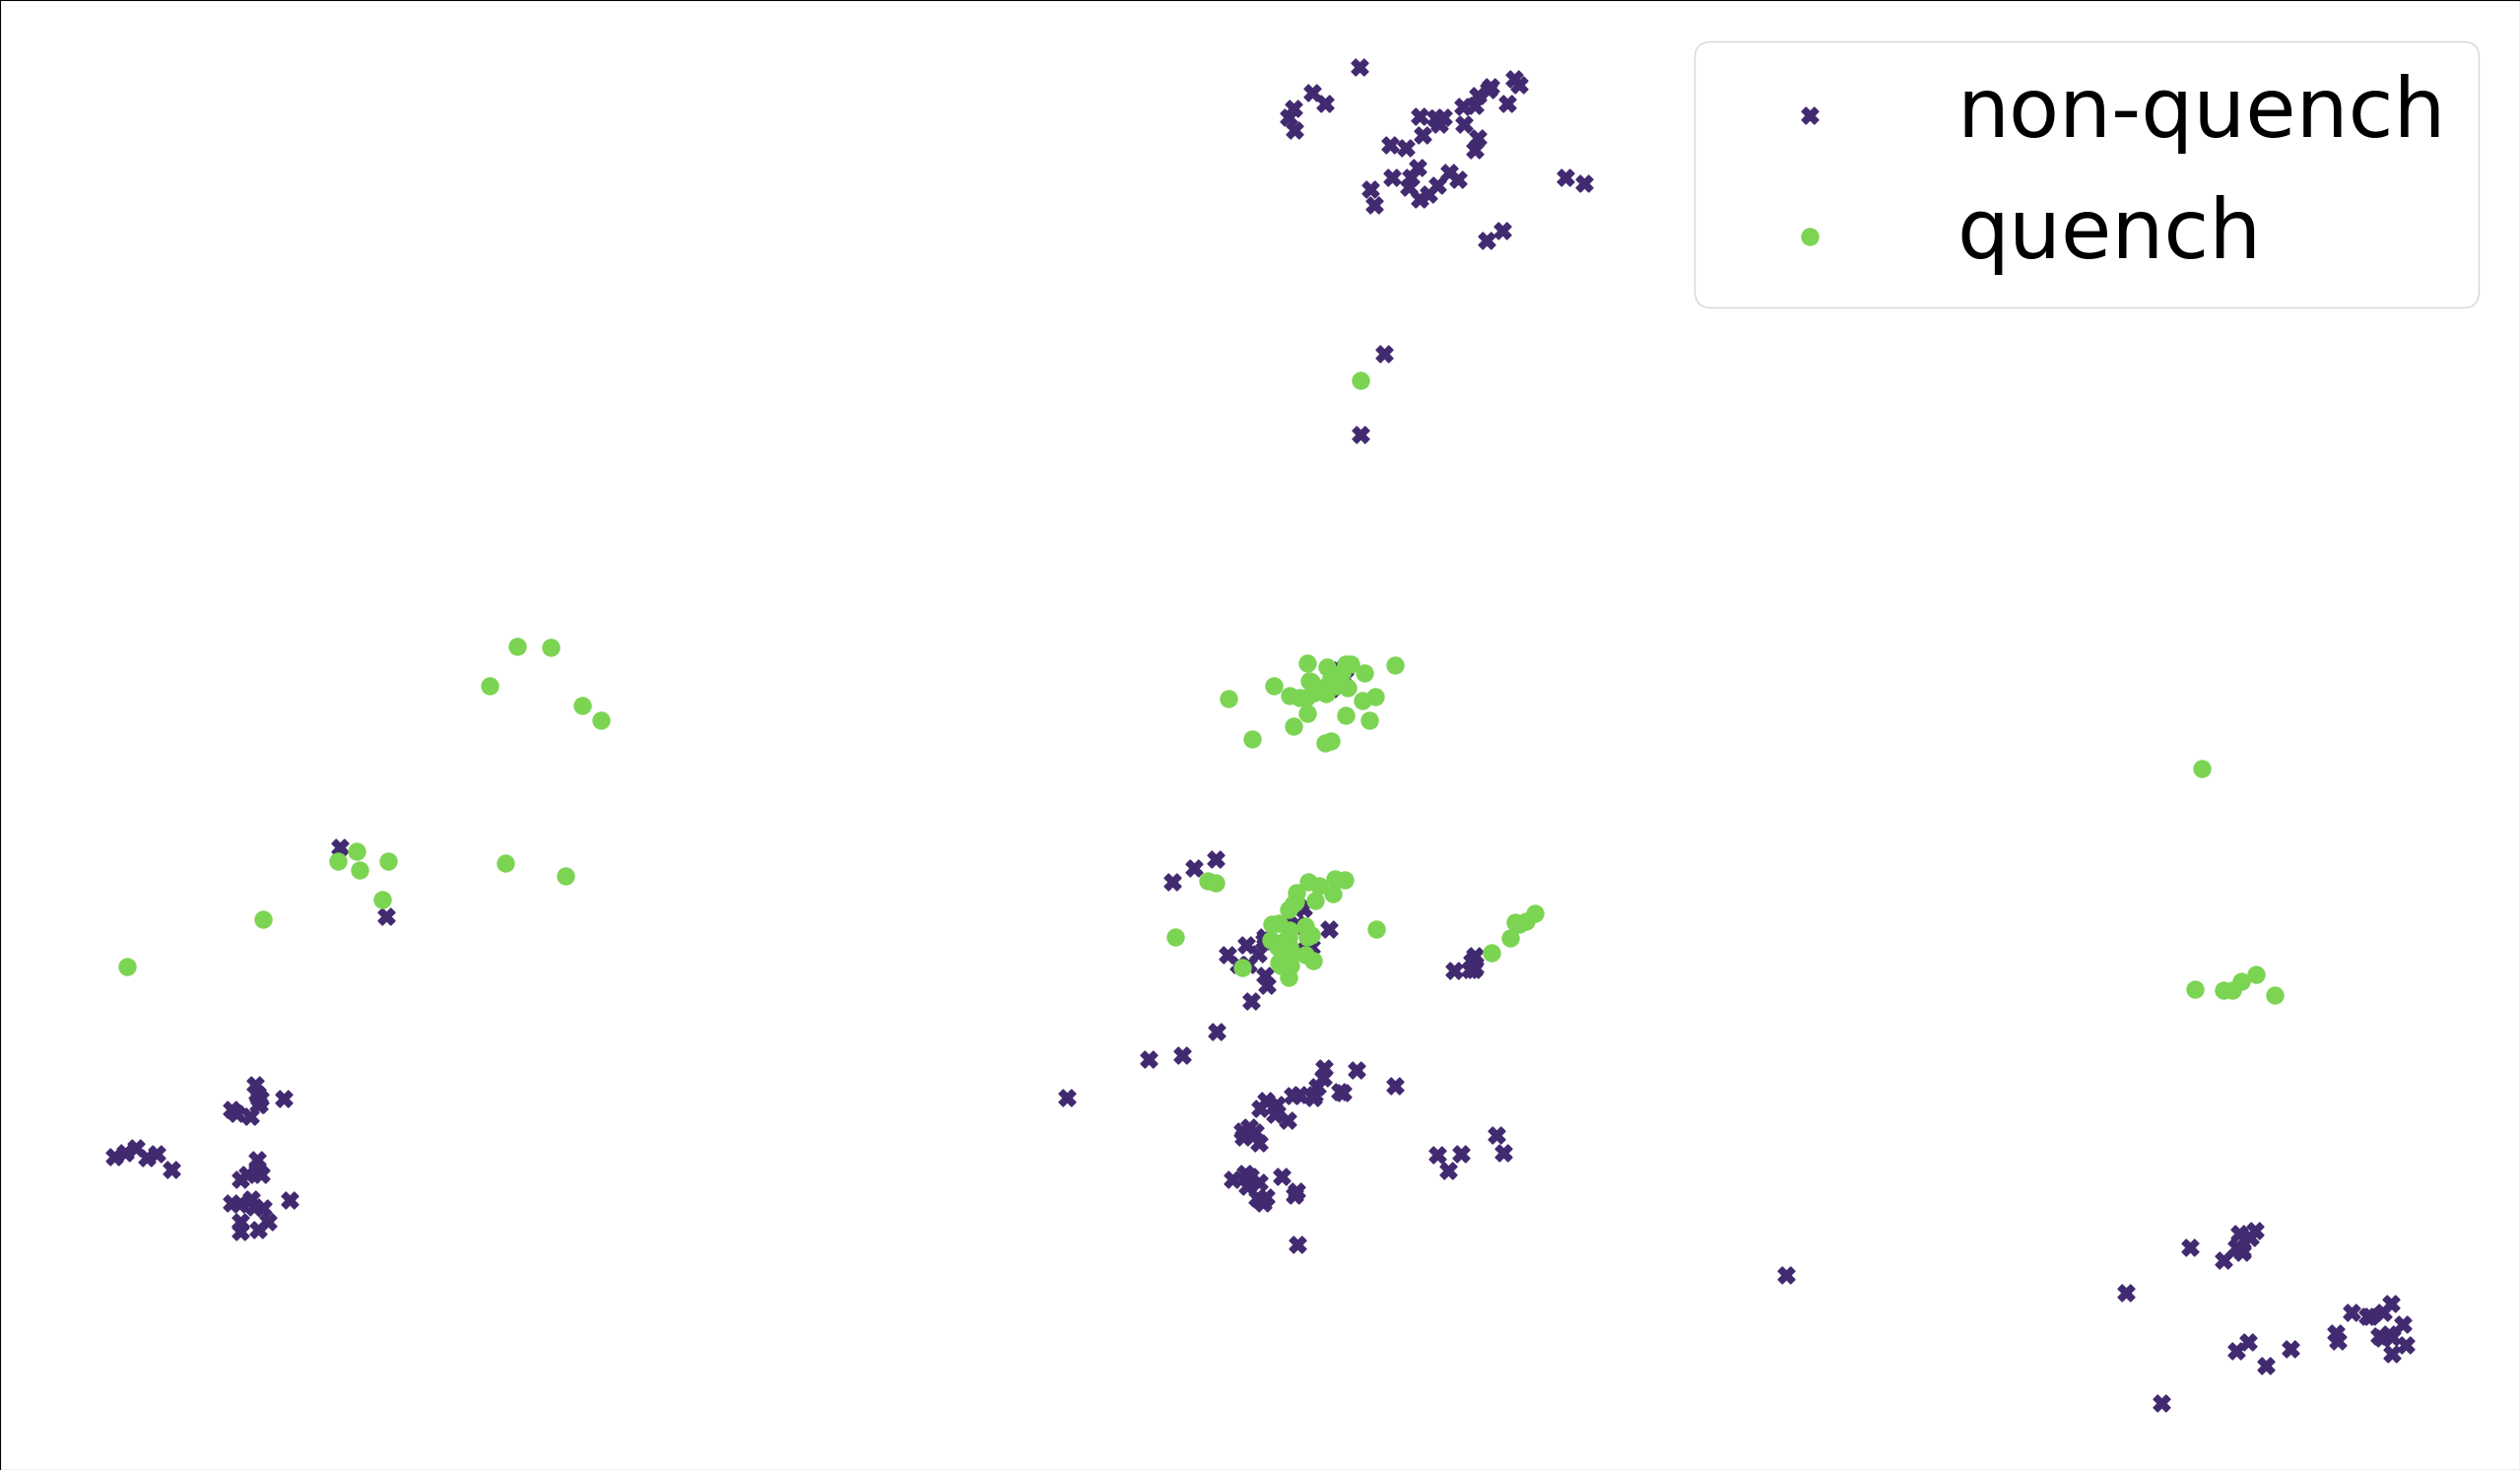
\includegraphics[width=\linewidth]{img/quench_dist_qlp/quenches_coil_1_An.png}
		\subcaption{}
	\end{subfigure}
	\begin{subfigure}{0.49\linewidth}
		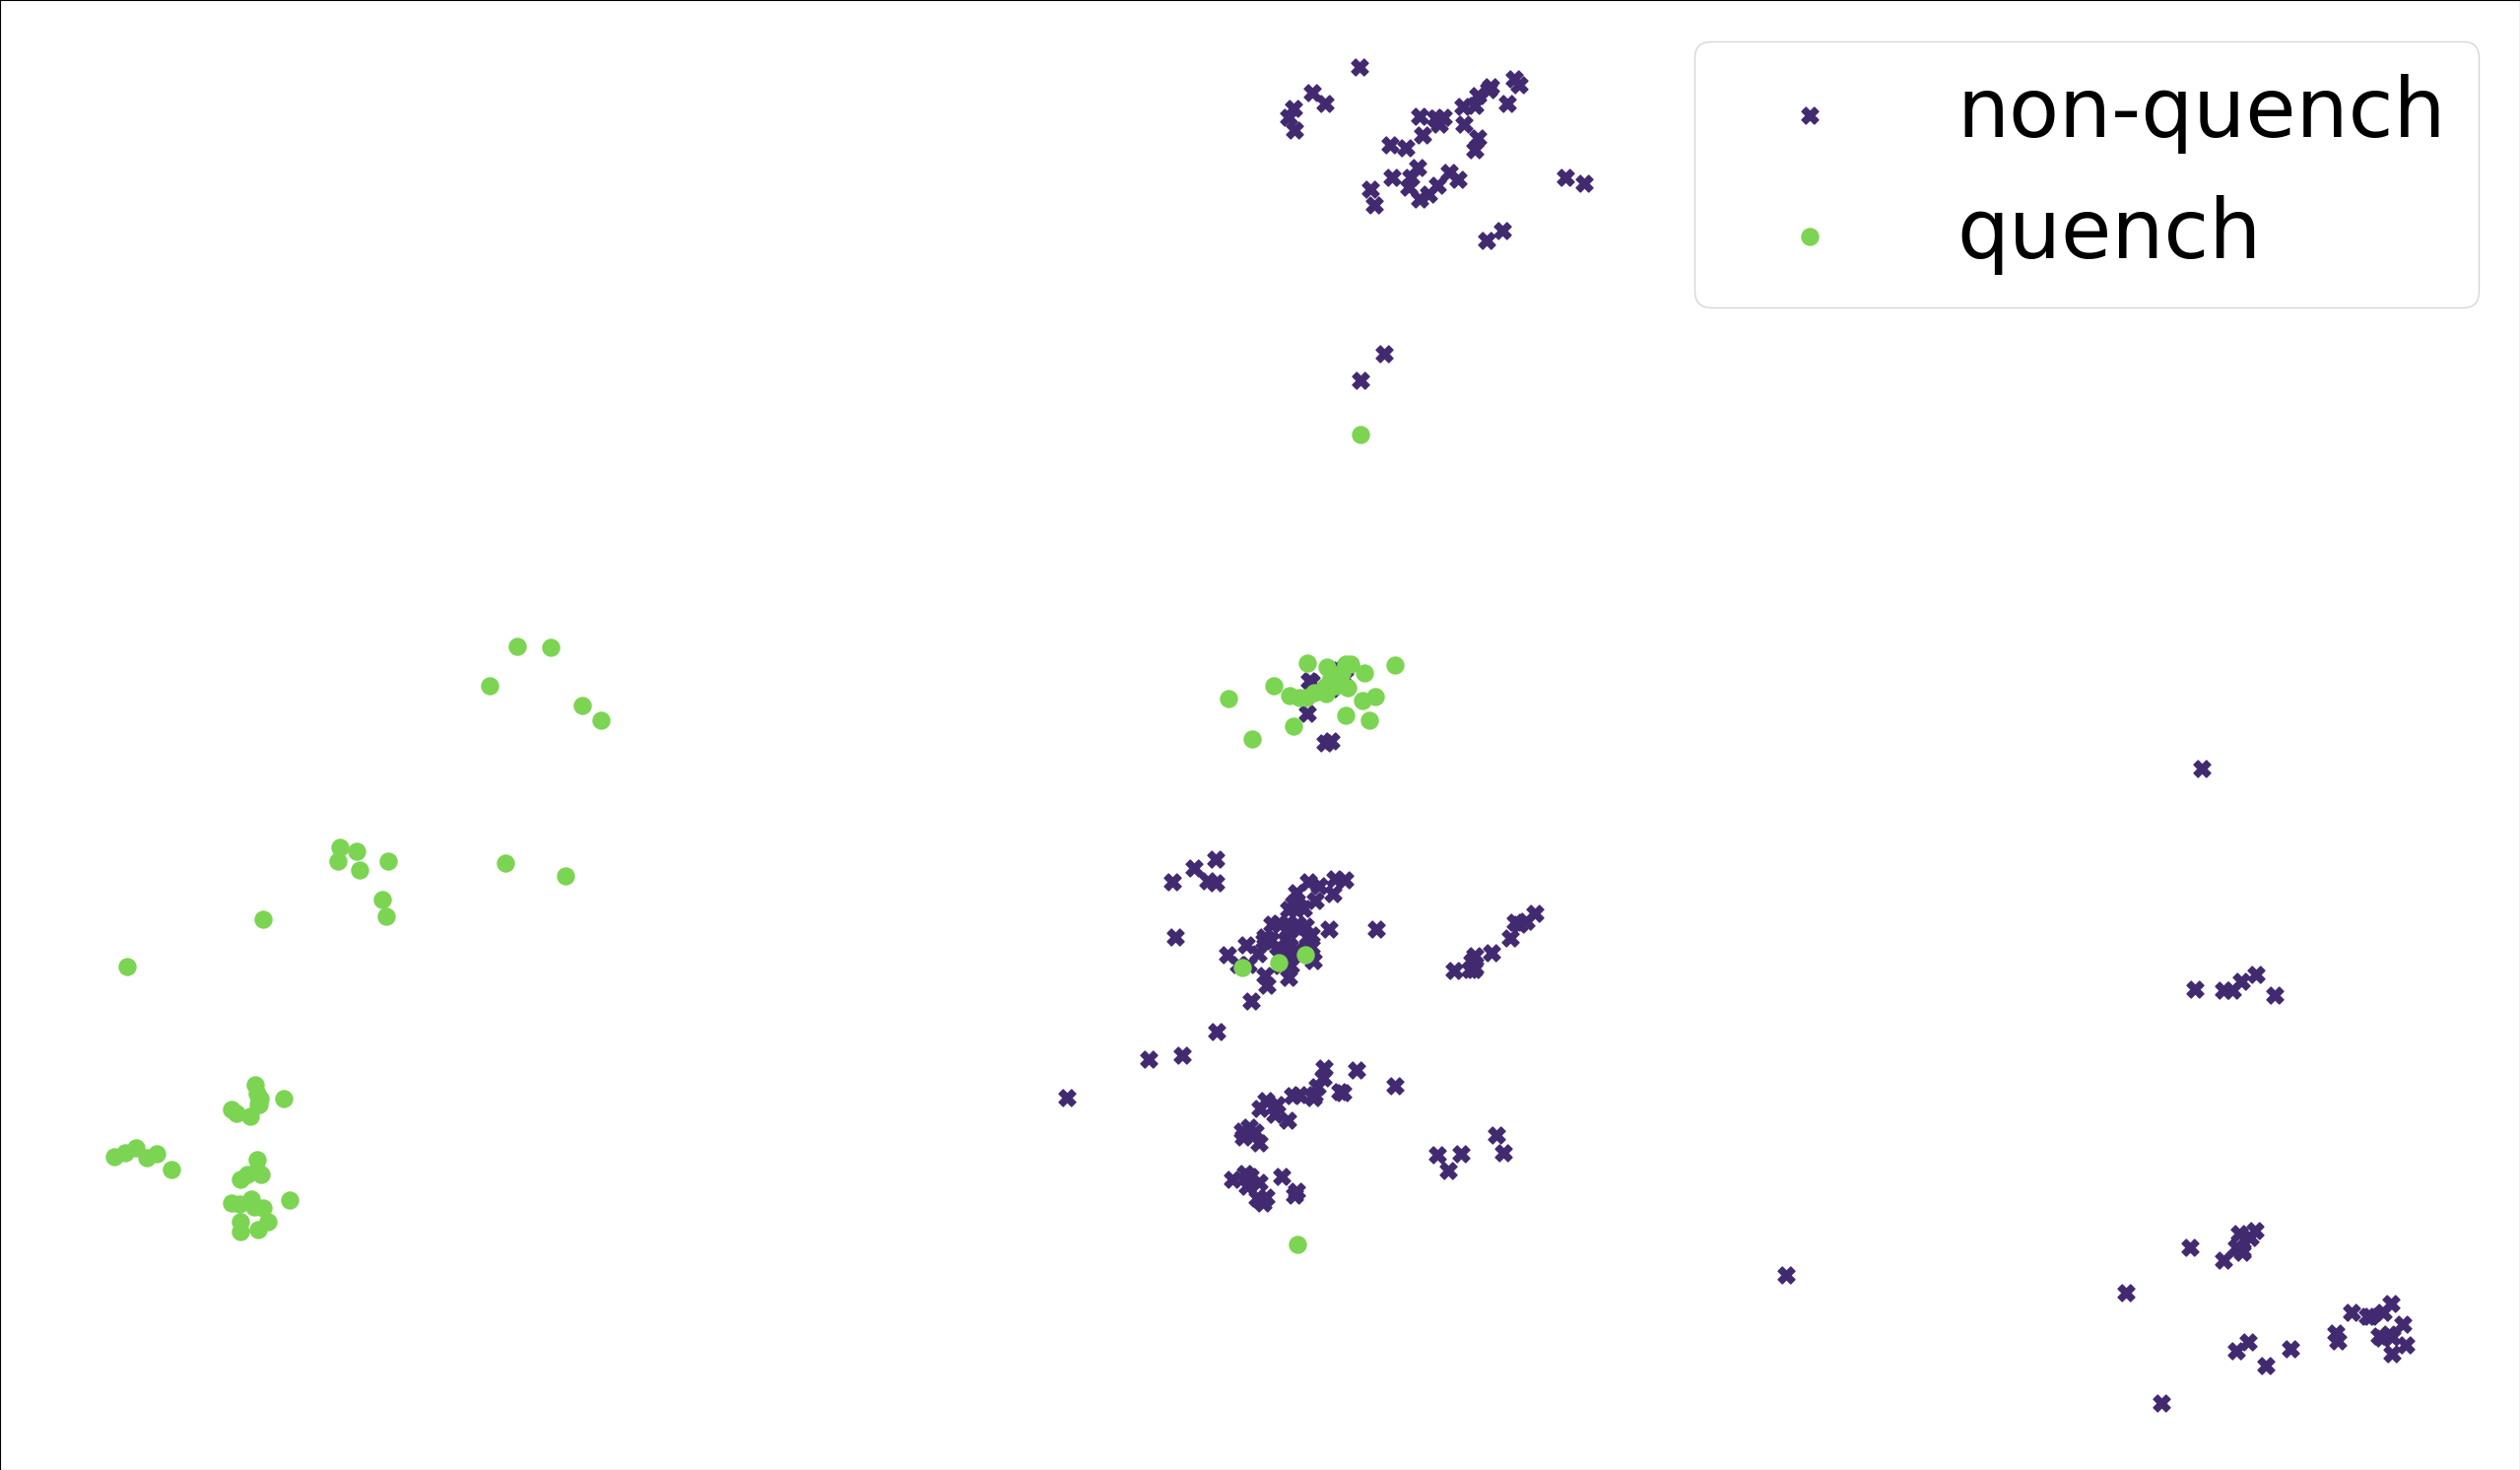
\includegraphics[width=\linewidth]{img/quench_dist_qlp/quenches_coil_2_An.png}
		\subcaption{}
	\end{subfigure}
	\begin{subfigure}{0.49\linewidth}
		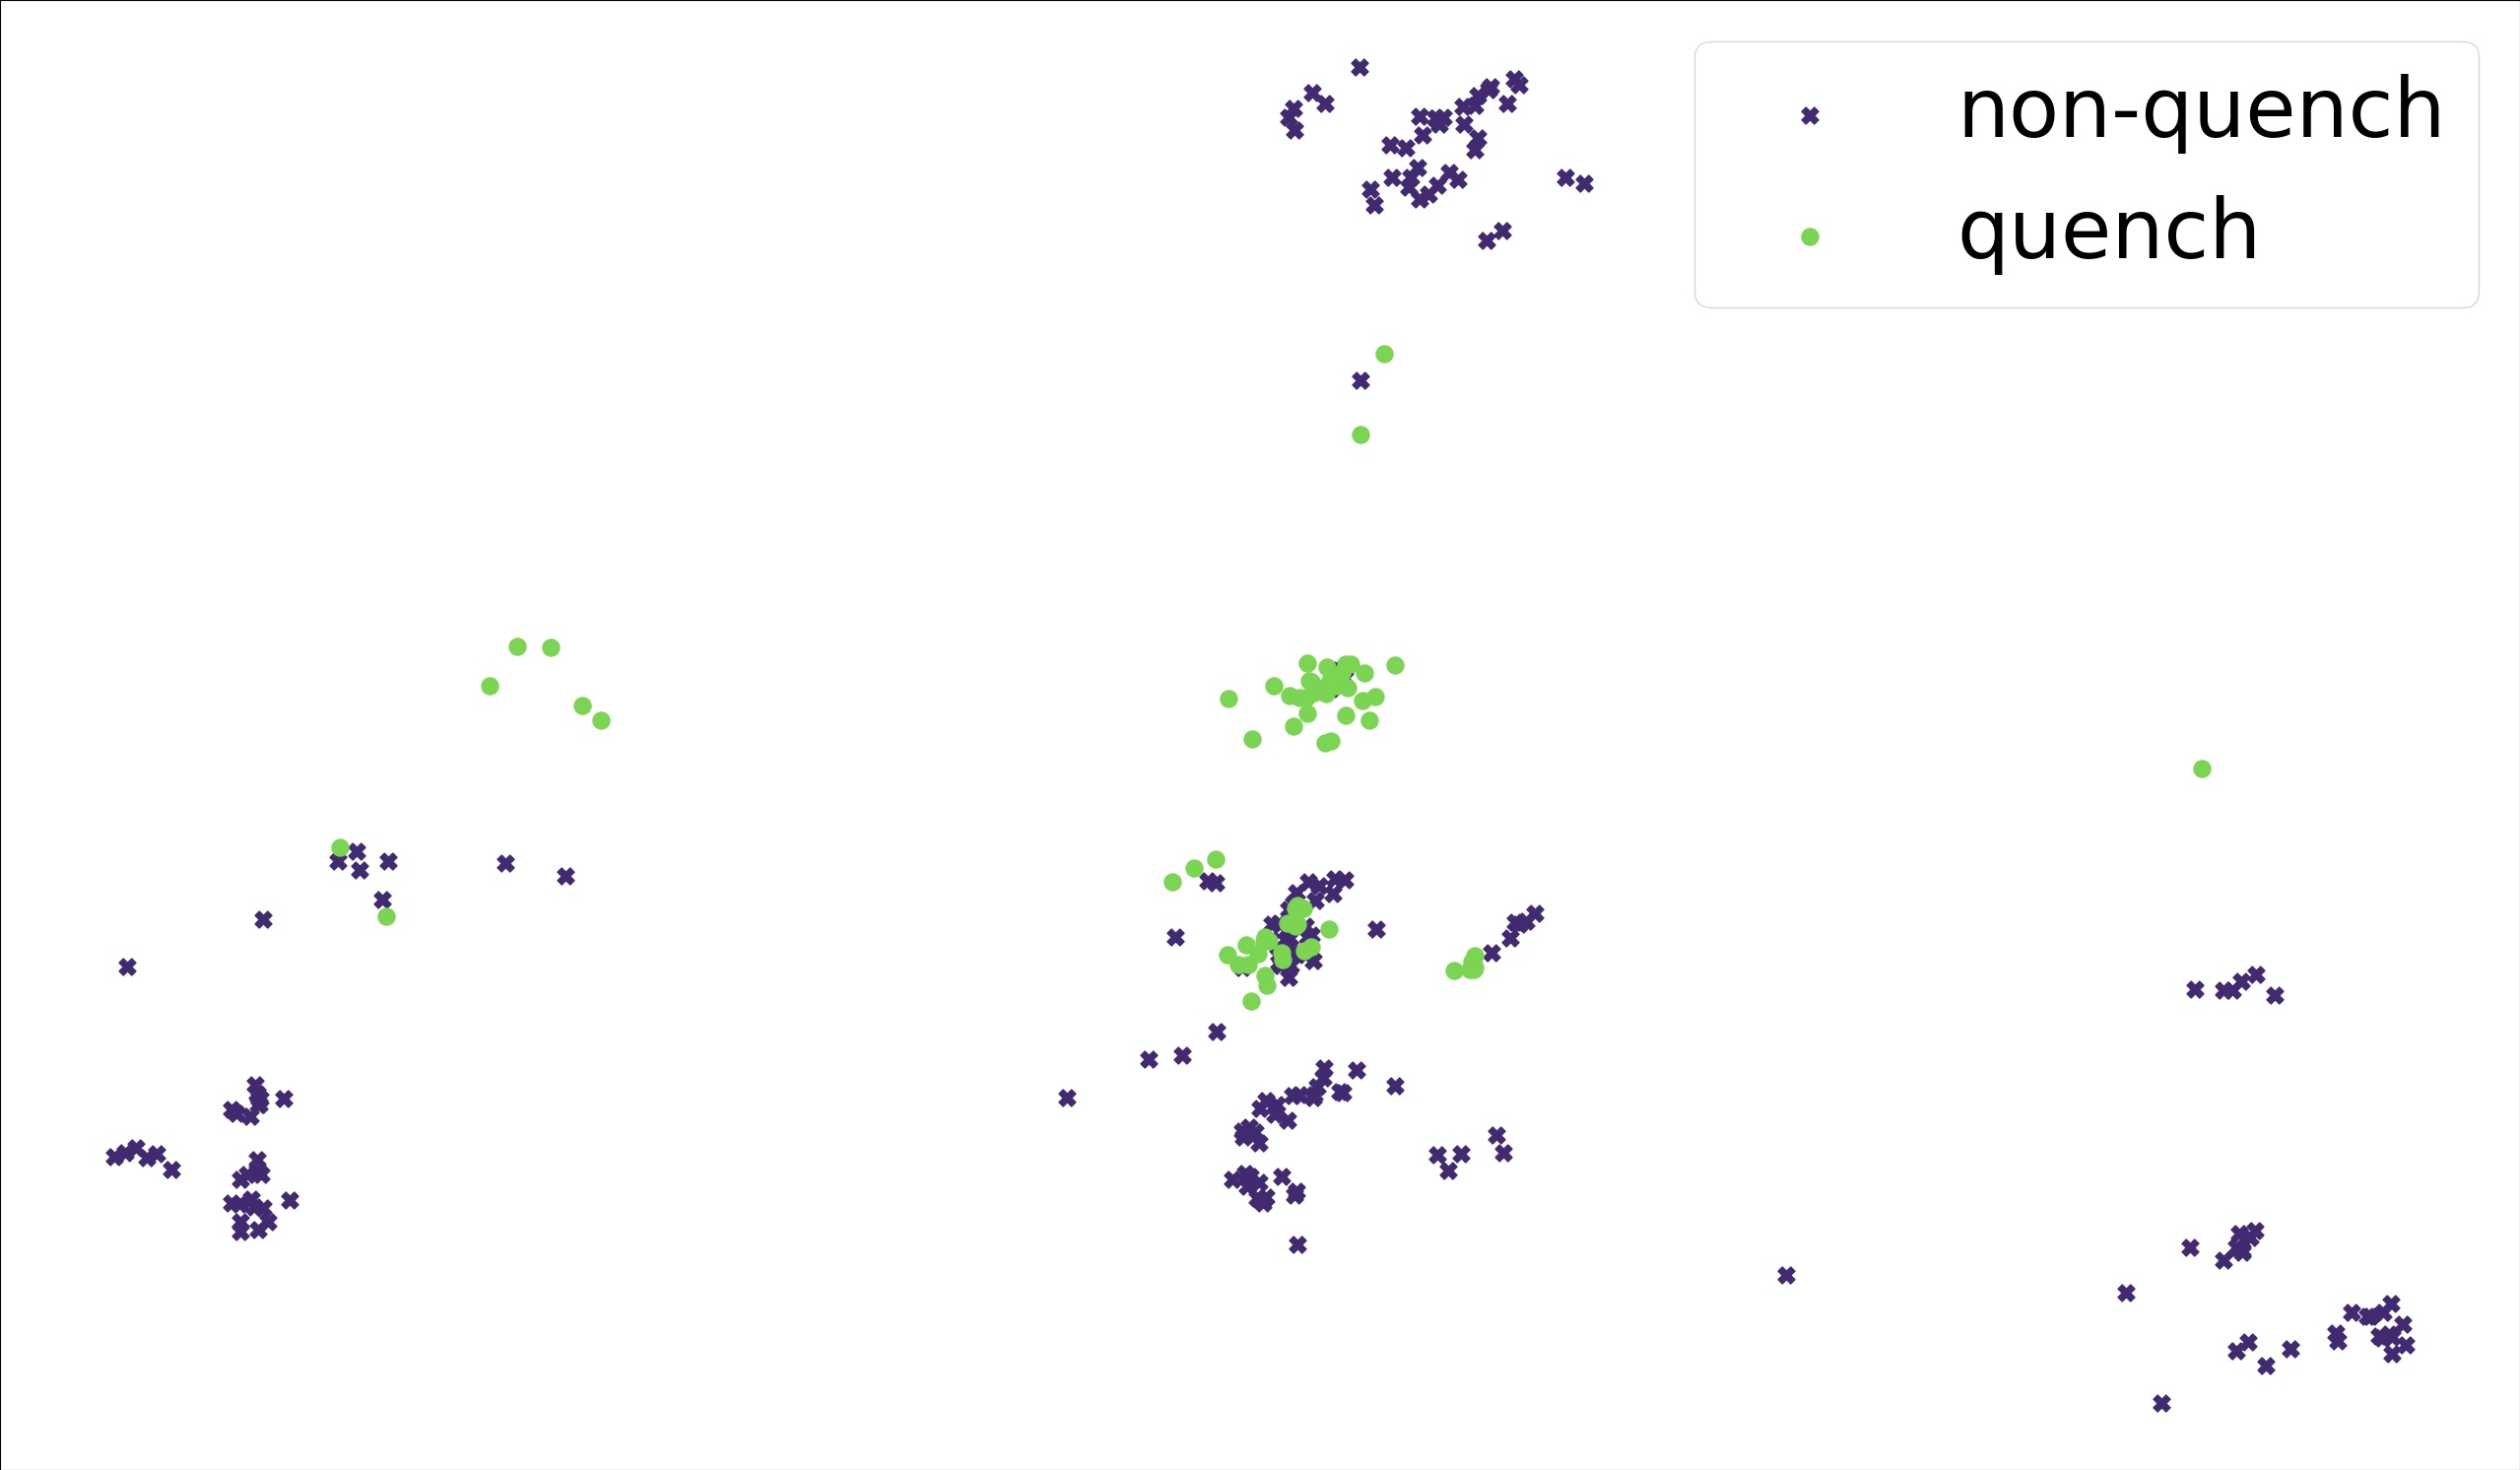
\includegraphics[width=\linewidth]{img/quench_dist_qlp/quenches_coil_3_An.png}
		\subcaption{}
	\end{subfigure}
	\caption{The distribution of the samples in bidimensional space after a round of \pca, for
		the \an\ attribute. The subfigures contain different views of the same data: (a) differenciates between non-quench and single or multiple quench events, (b) highlights the distribution of quenches for coil $0$, (c) highlights the distribution of quenches for coil $1$, (d) highlights the distribution of quenches for coil $2$ and finally (e) highlights the distribution of quenches for coil $3$.}
	\label{fig:an-coilq-dist}
\end{figure}

\subsubsection{\bn}
In \qrp\ \bn\ was the worst attribute among the ones we could choose, containing very low amounts of information and
having a high level of clutter in the data distribution (see \Cref{fig:bn-dist}). If we consider the
correlation between the attribute and the labels associated to every coil, \Cref{fig:bn-lcorr-qlp},
we can see that the attribute has a strong correlation with coils $1$ and $3$, with the same pattern
highlighted in the case of \an, and shown in figure \Cref{fig:an-lcorr-qlp}. Sub-views of \bn\ would be built following the same structure outlined for \an.

\begin{figure}[!h]
	% Font size = 70
	\centering
	\begin{subfigure}{0.49\linewidth}
		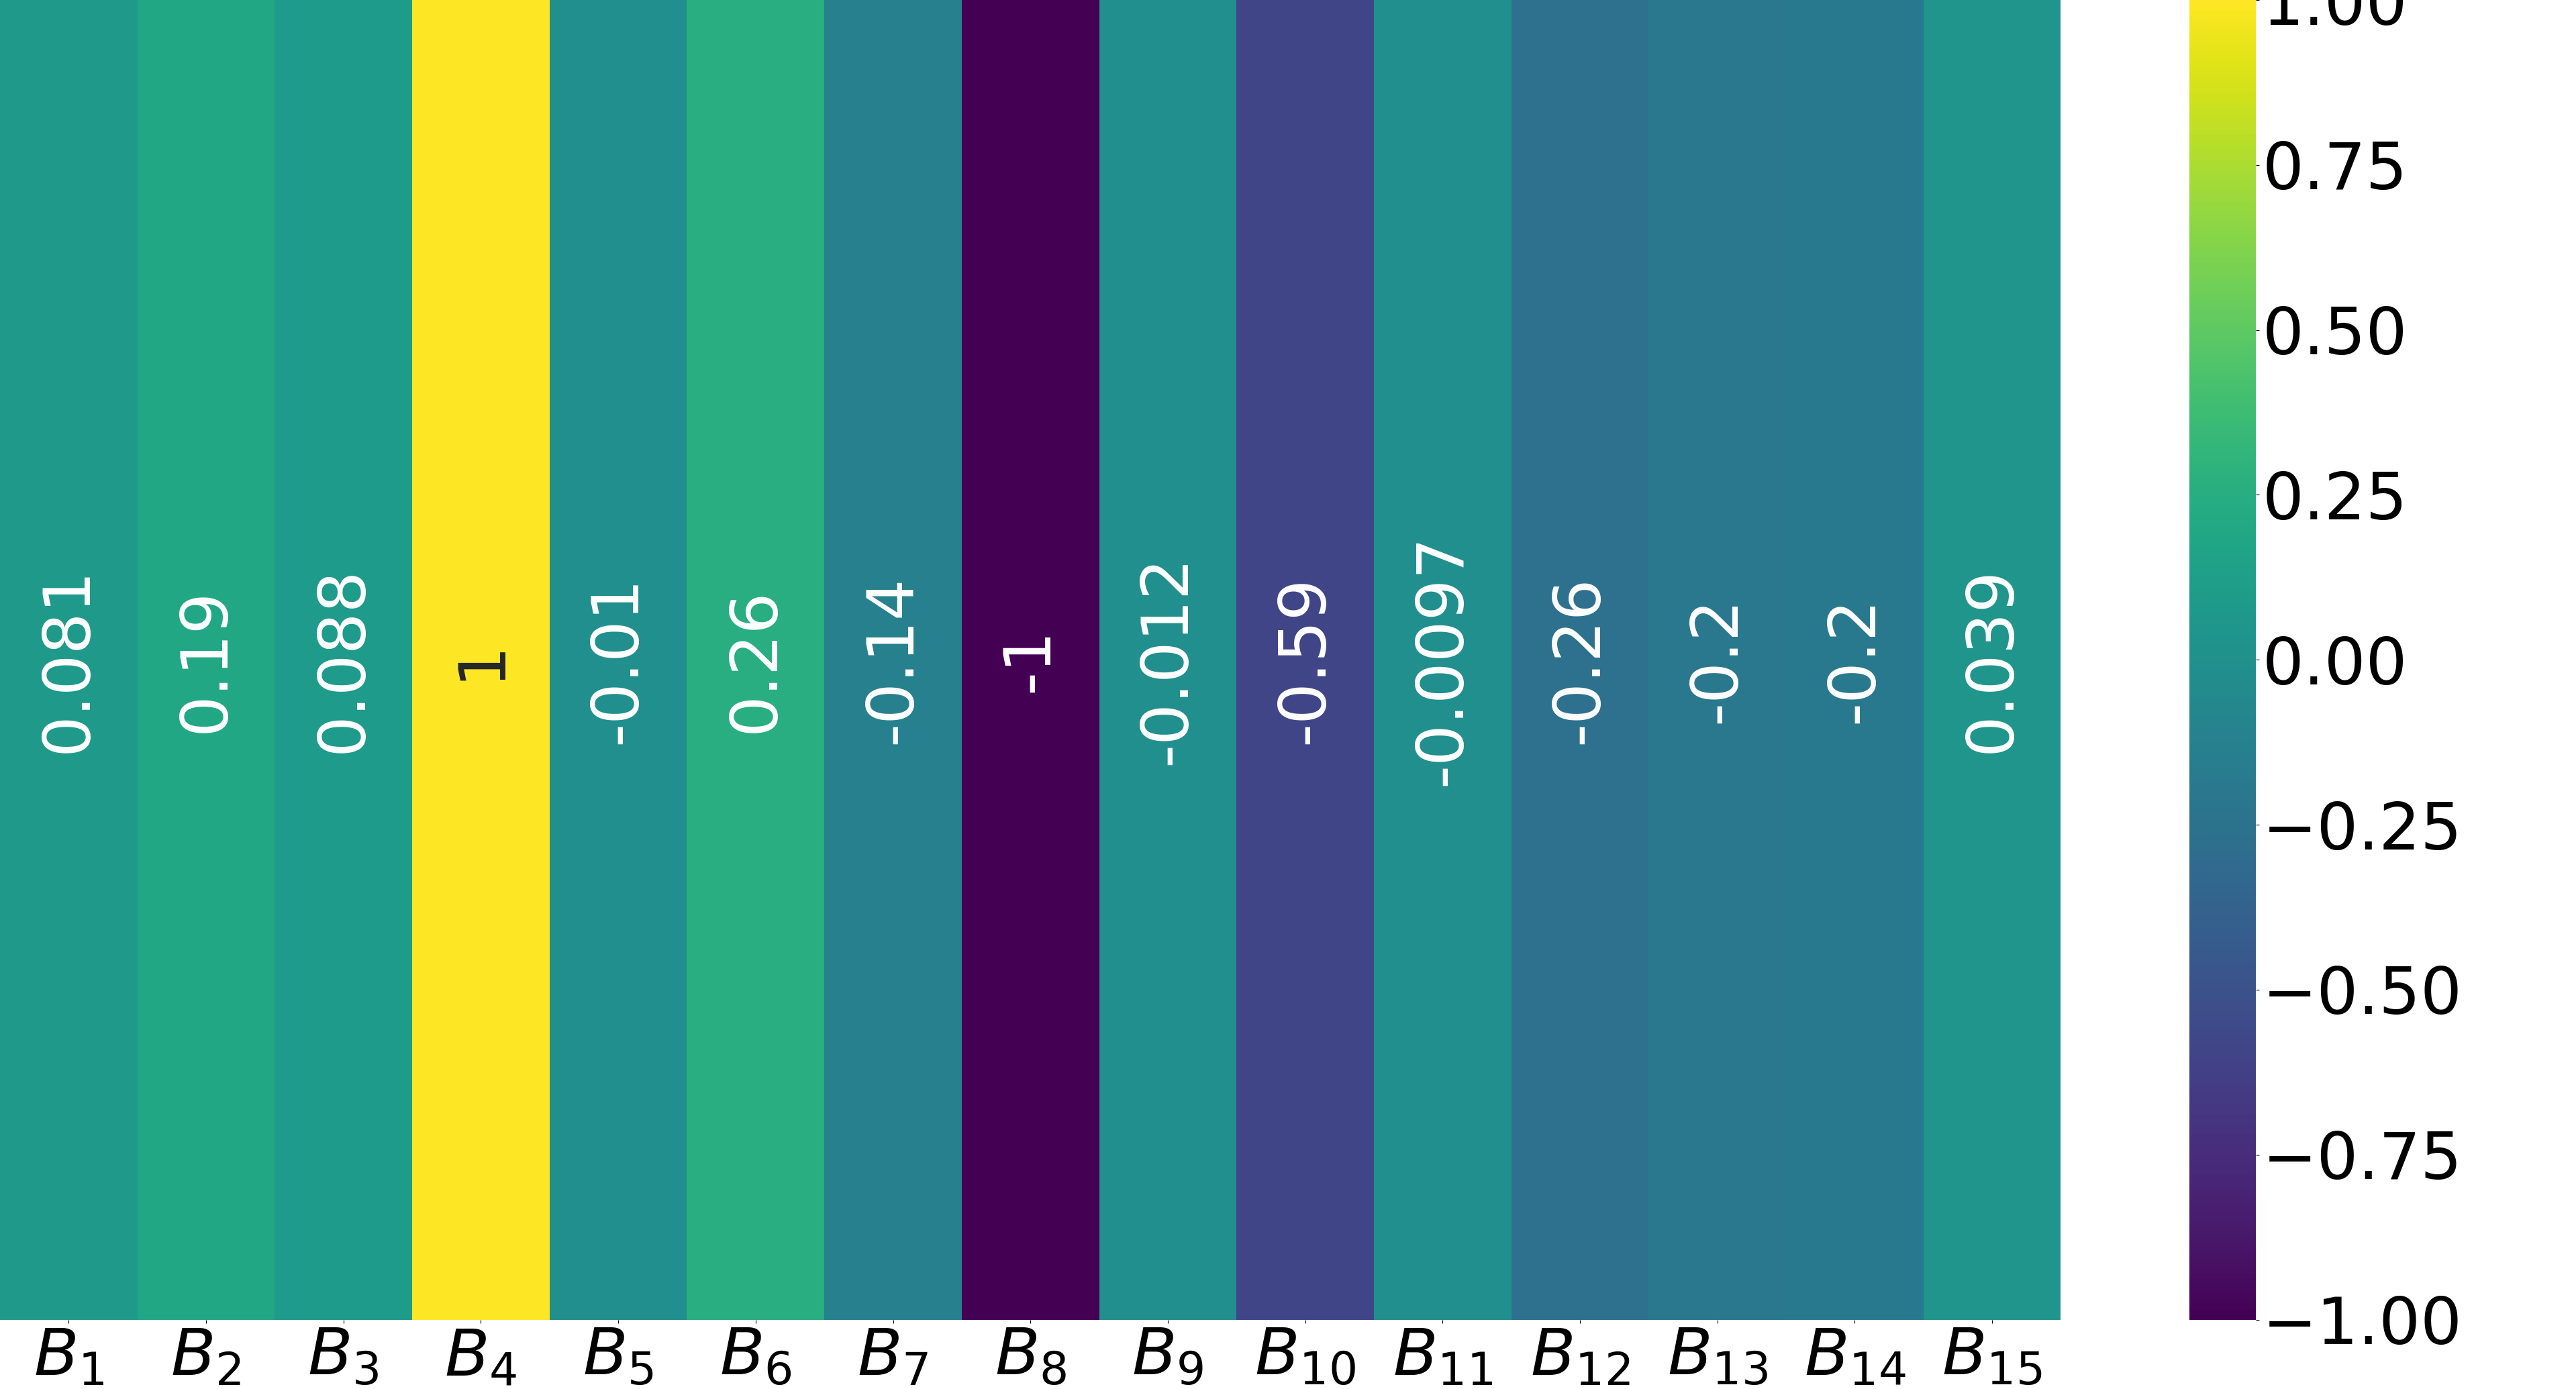
\includegraphics[width=\linewidth]{img/qlp_corr/Bn_coil0.png}
		\subcaption{Correlation with coil $0$}
	\end{subfigure}
	\begin{subfigure}{0.49\linewidth}
		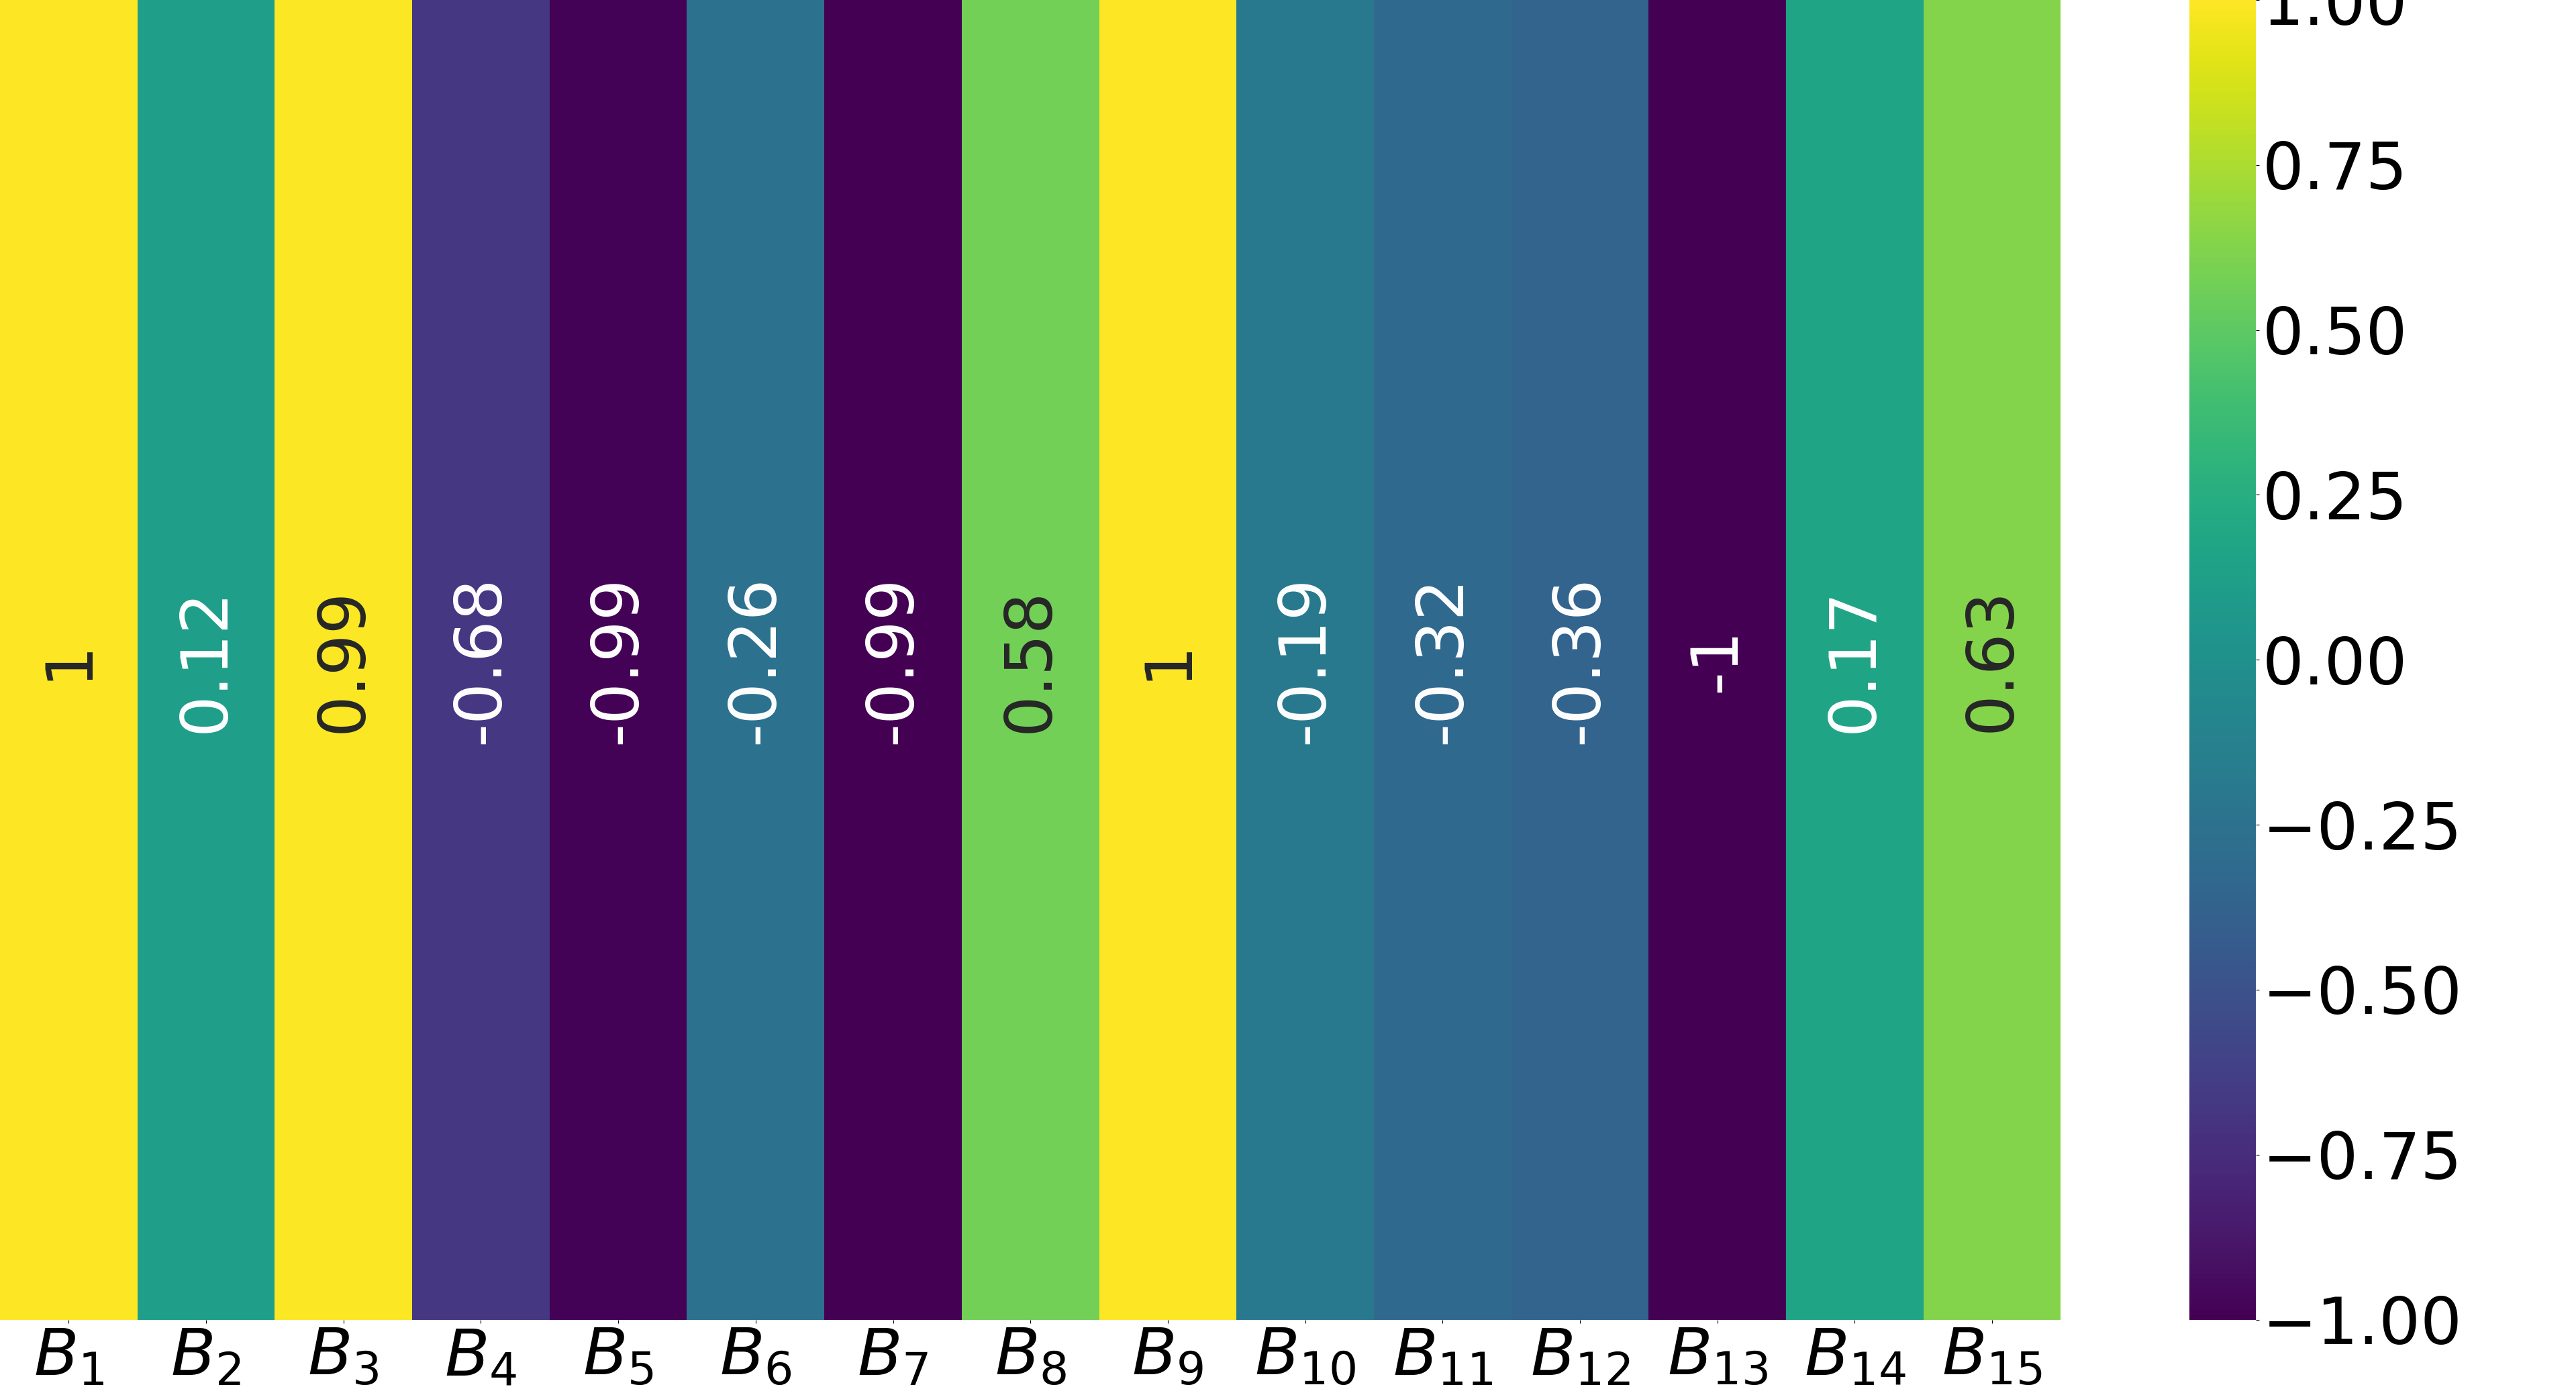
\includegraphics[width=\linewidth]{img/qlp_corr/Bn_coil1.png}
		\subcaption{Correlation with coil $1$}
	\end{subfigure}
	\begin{subfigure}{0.49\linewidth}
		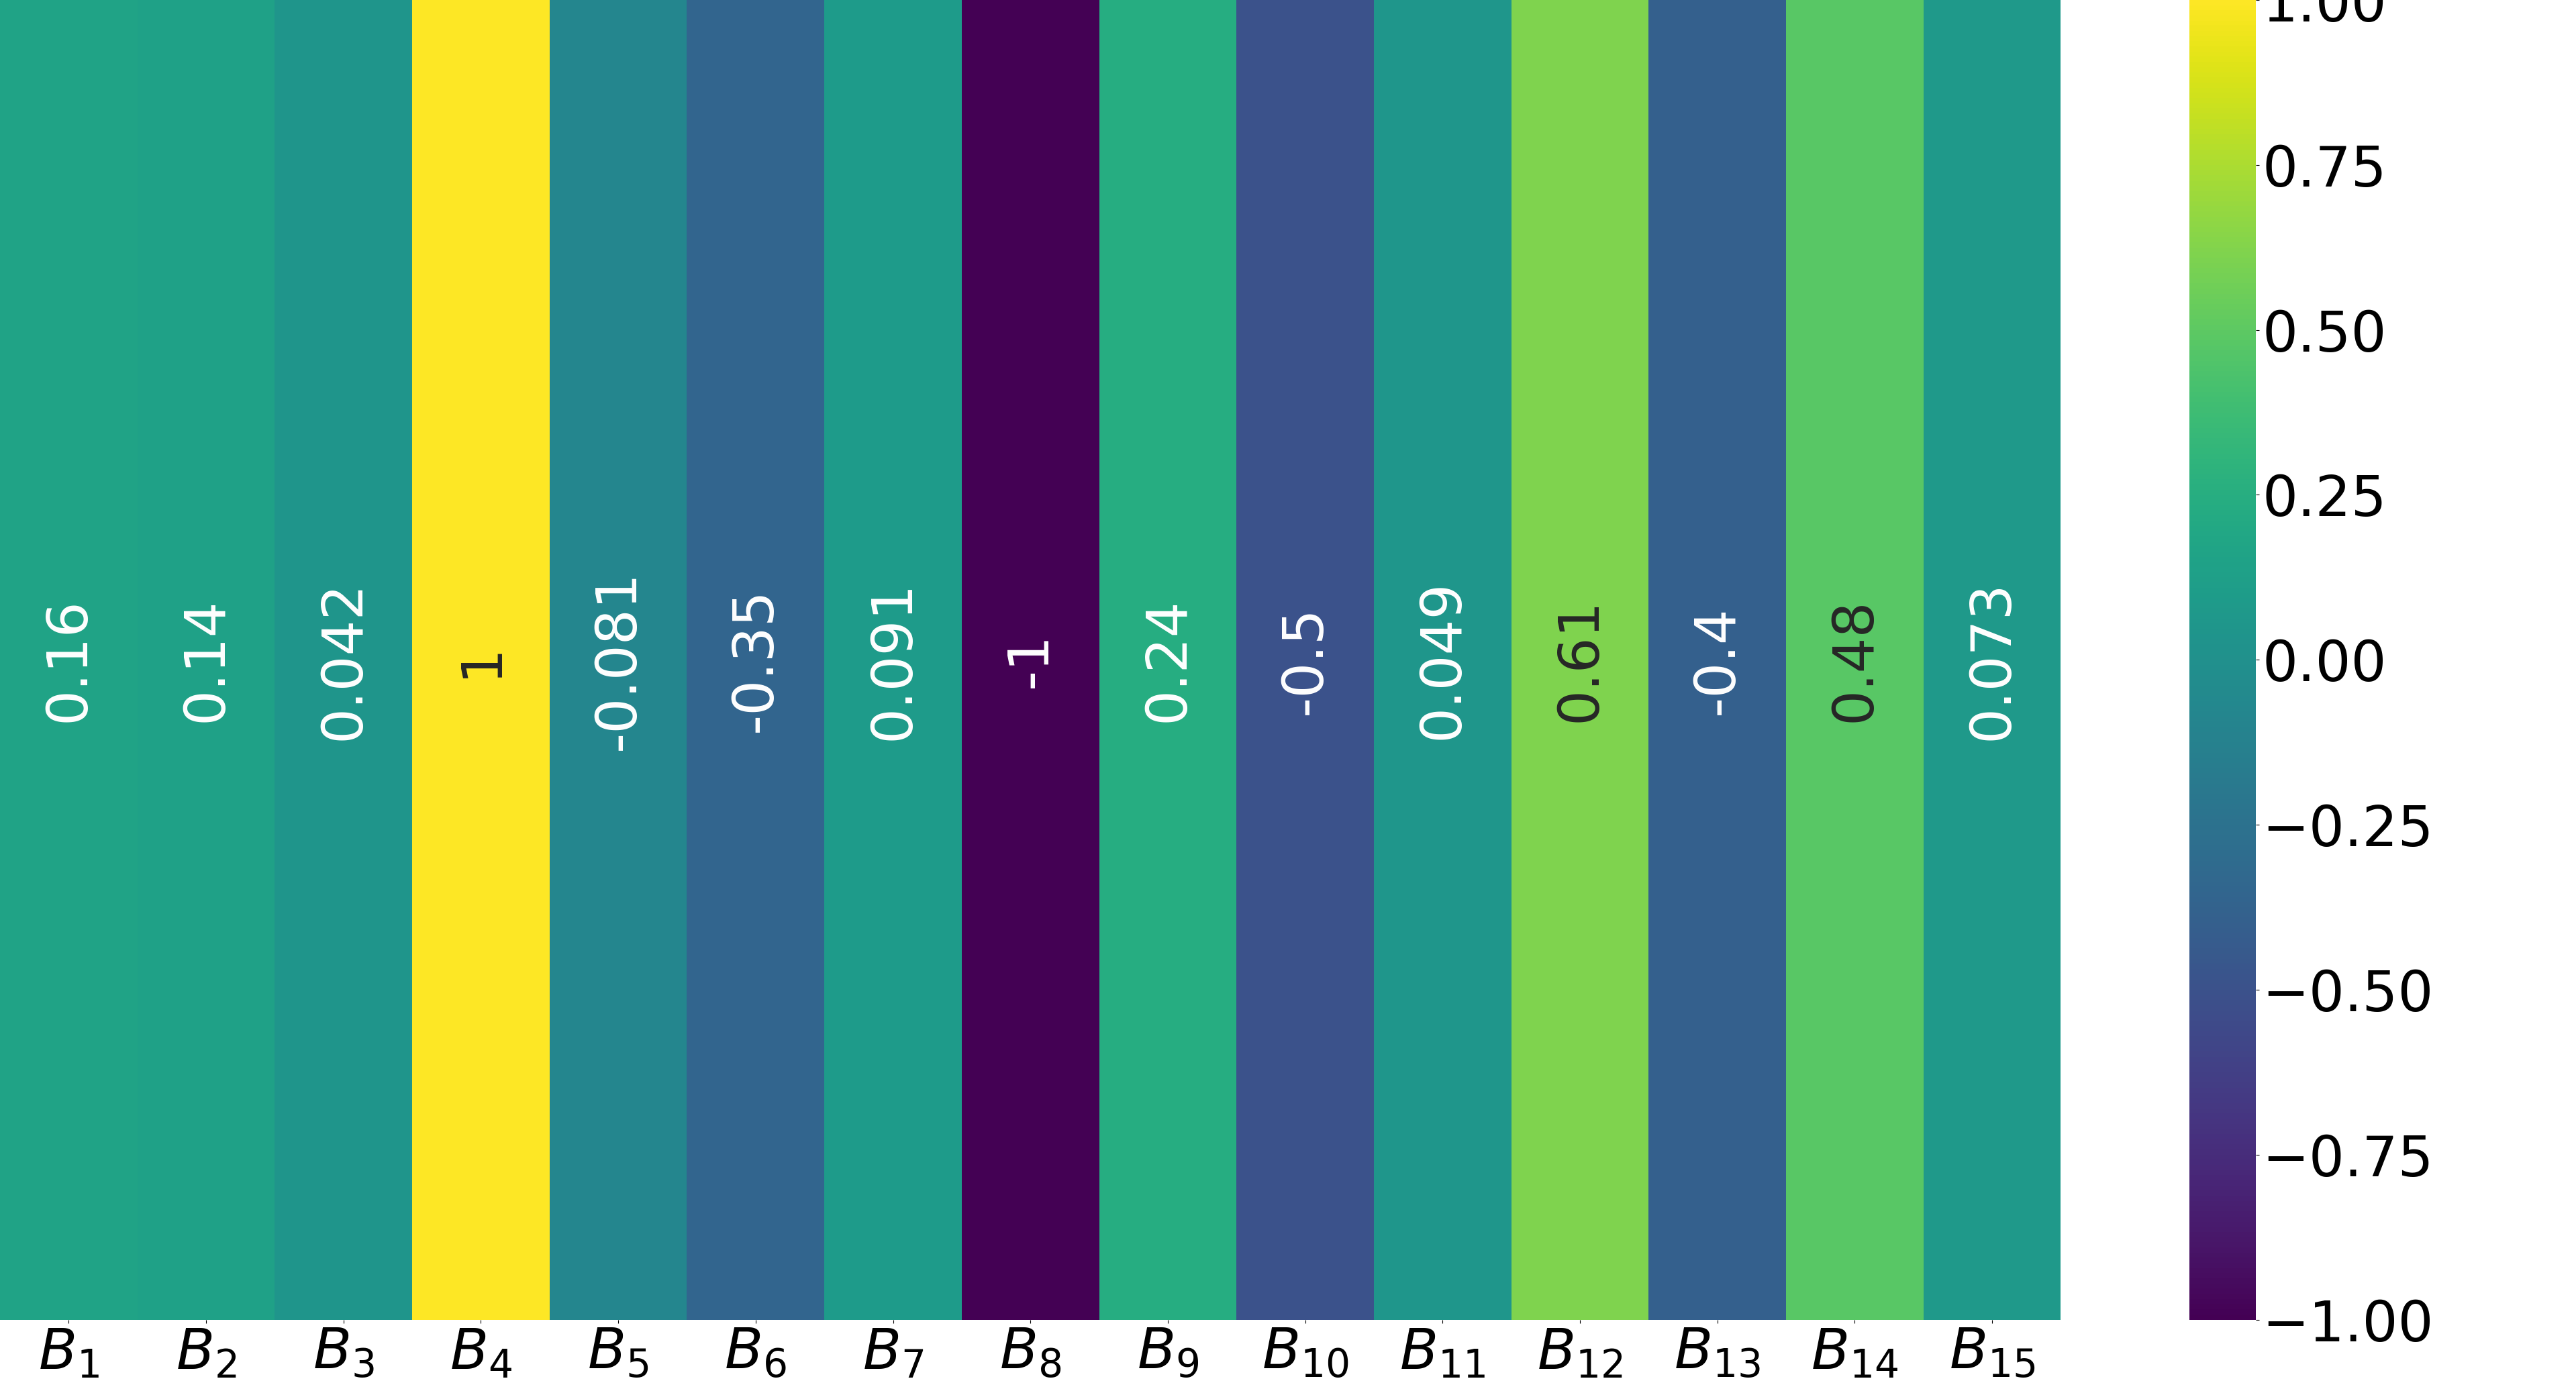
\includegraphics[width=\linewidth]{img/qlp_corr/Bn_coil2.png}
		\subcaption{Correlation with coil $2$}
	\end{subfigure}
	\begin{subfigure}{0.49\linewidth}
		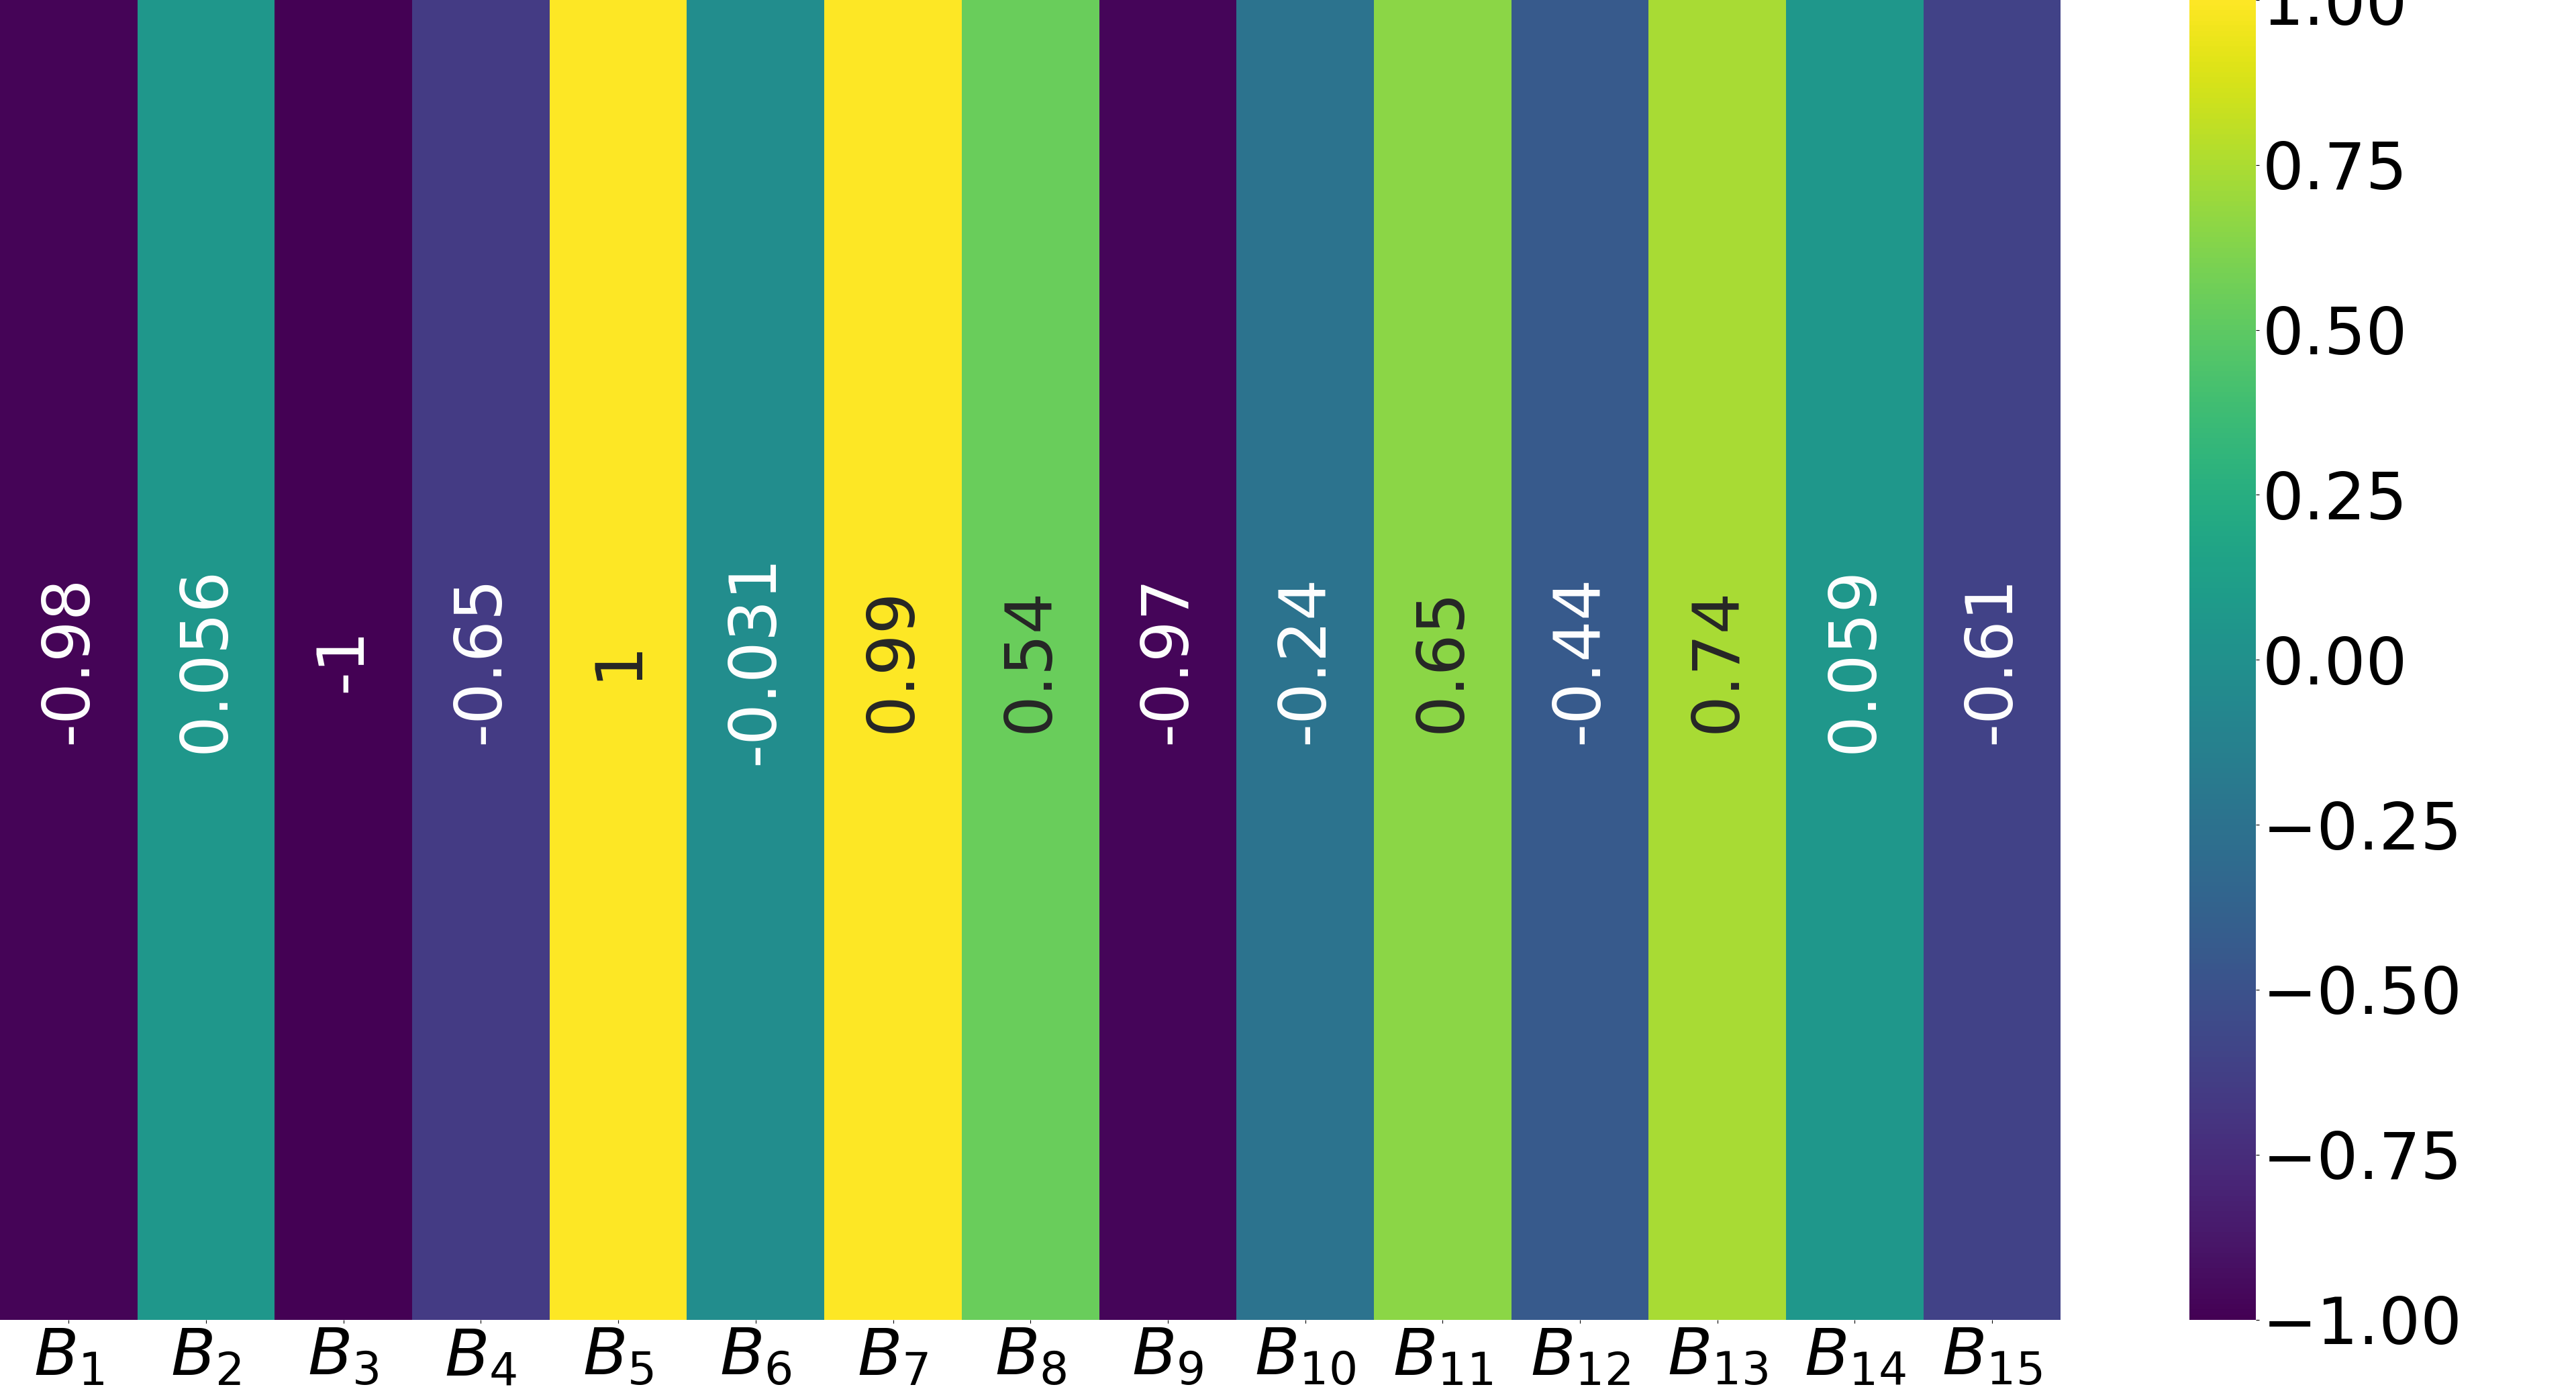
\includegraphics[width=\linewidth]{img/qlp_corr/Bn_coil3.png}
		\subcaption{Correlation with coil $3$}
	\end{subfigure}
	\caption{Correlation between the harmonics of the \bn\ attribute and the labels for \qlp.}
	\label{fig:bn-lcorr-qlp}
\end{figure}

In \Cref{fig:bn-coilq-dist} we highlight, once again, the distribution of the samples after a round
of \pca, as we can see in subfigure (a) the distribution of samples representing non-quench and
single or multiple quench events is very confusing, there is a central cluster with a high degree of
noise, meanwhile the side clusters seem to have higher purity, but compared with the distribution of
the \an\ attribute we are as close to unusable as it gets. Looking at the distribution of the data
for single coils it's quite clear that, once again, the separation of the classes is not at the level
of \an, which is proving to be better (at least qualitatively) but we can see that there is a
certain degree of separation (especially in subfigures (c) and (e)) between non-quench and quench
classes.

\begin{figure}[!h]
	% Font size = 70
	\centering
	\begin{subfigure}{\linewidth}
		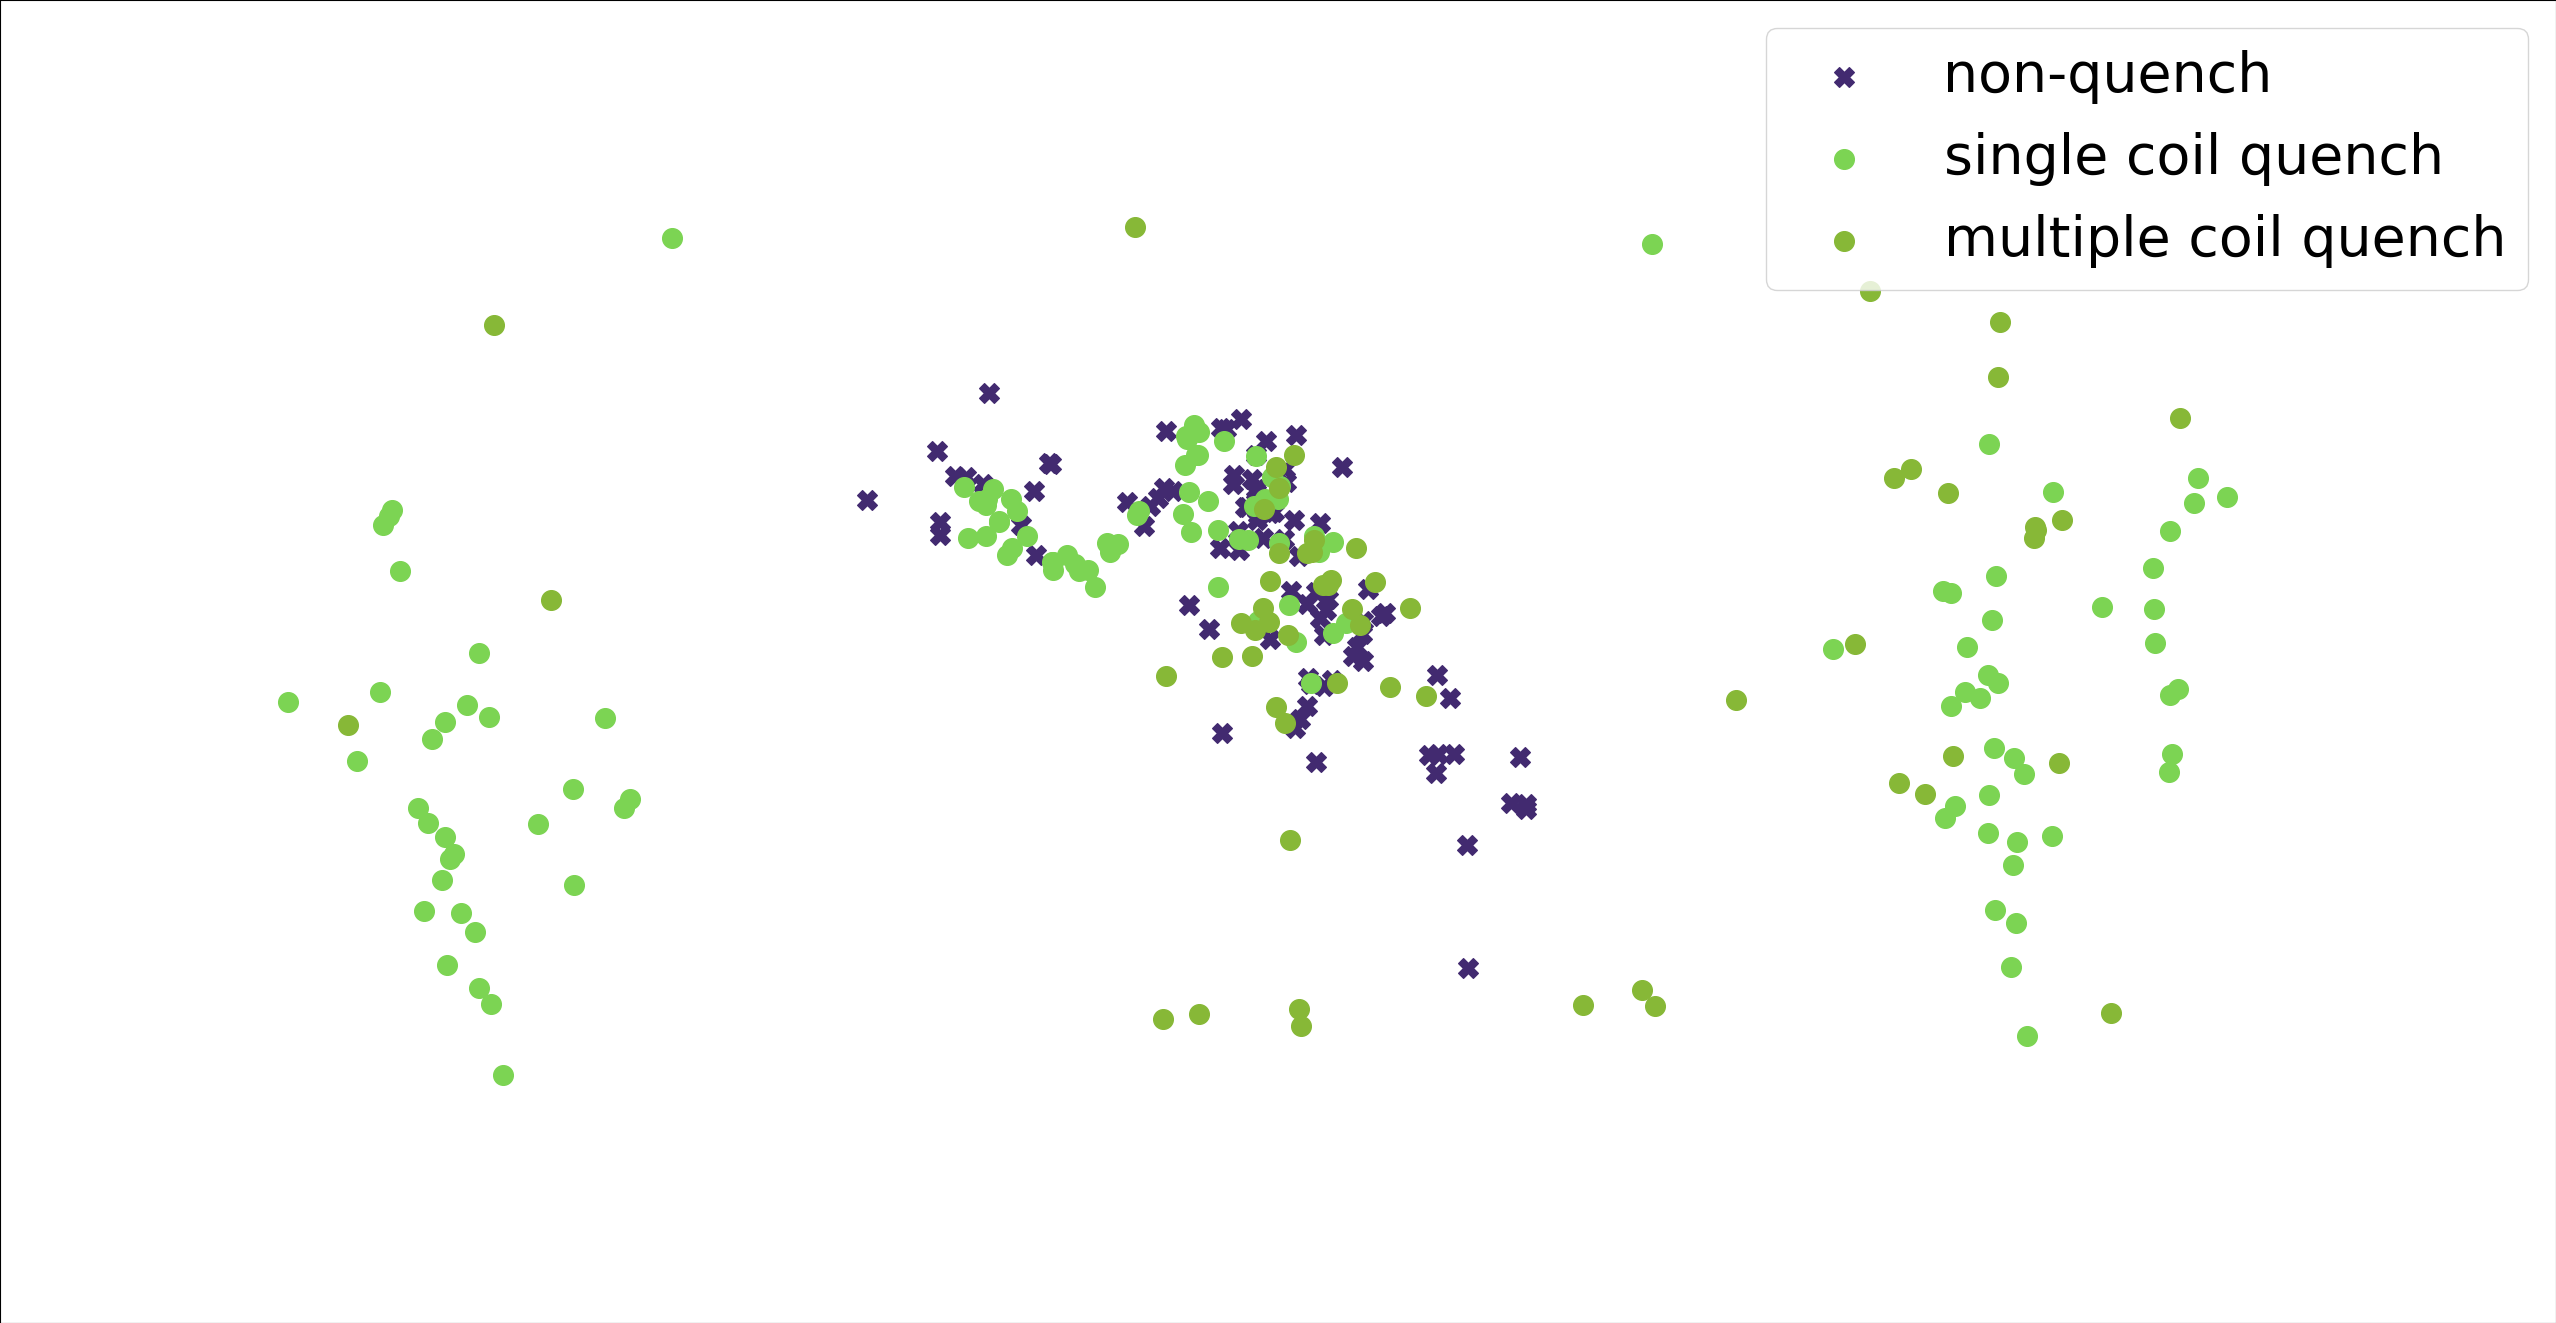
\includegraphics[width=\linewidth]{img/quench_dist_qlp/single_vs_multiple_Bn.png}
		\subcaption{}
	\end{subfigure}
	\begin{subfigure}{0.49\linewidth}
		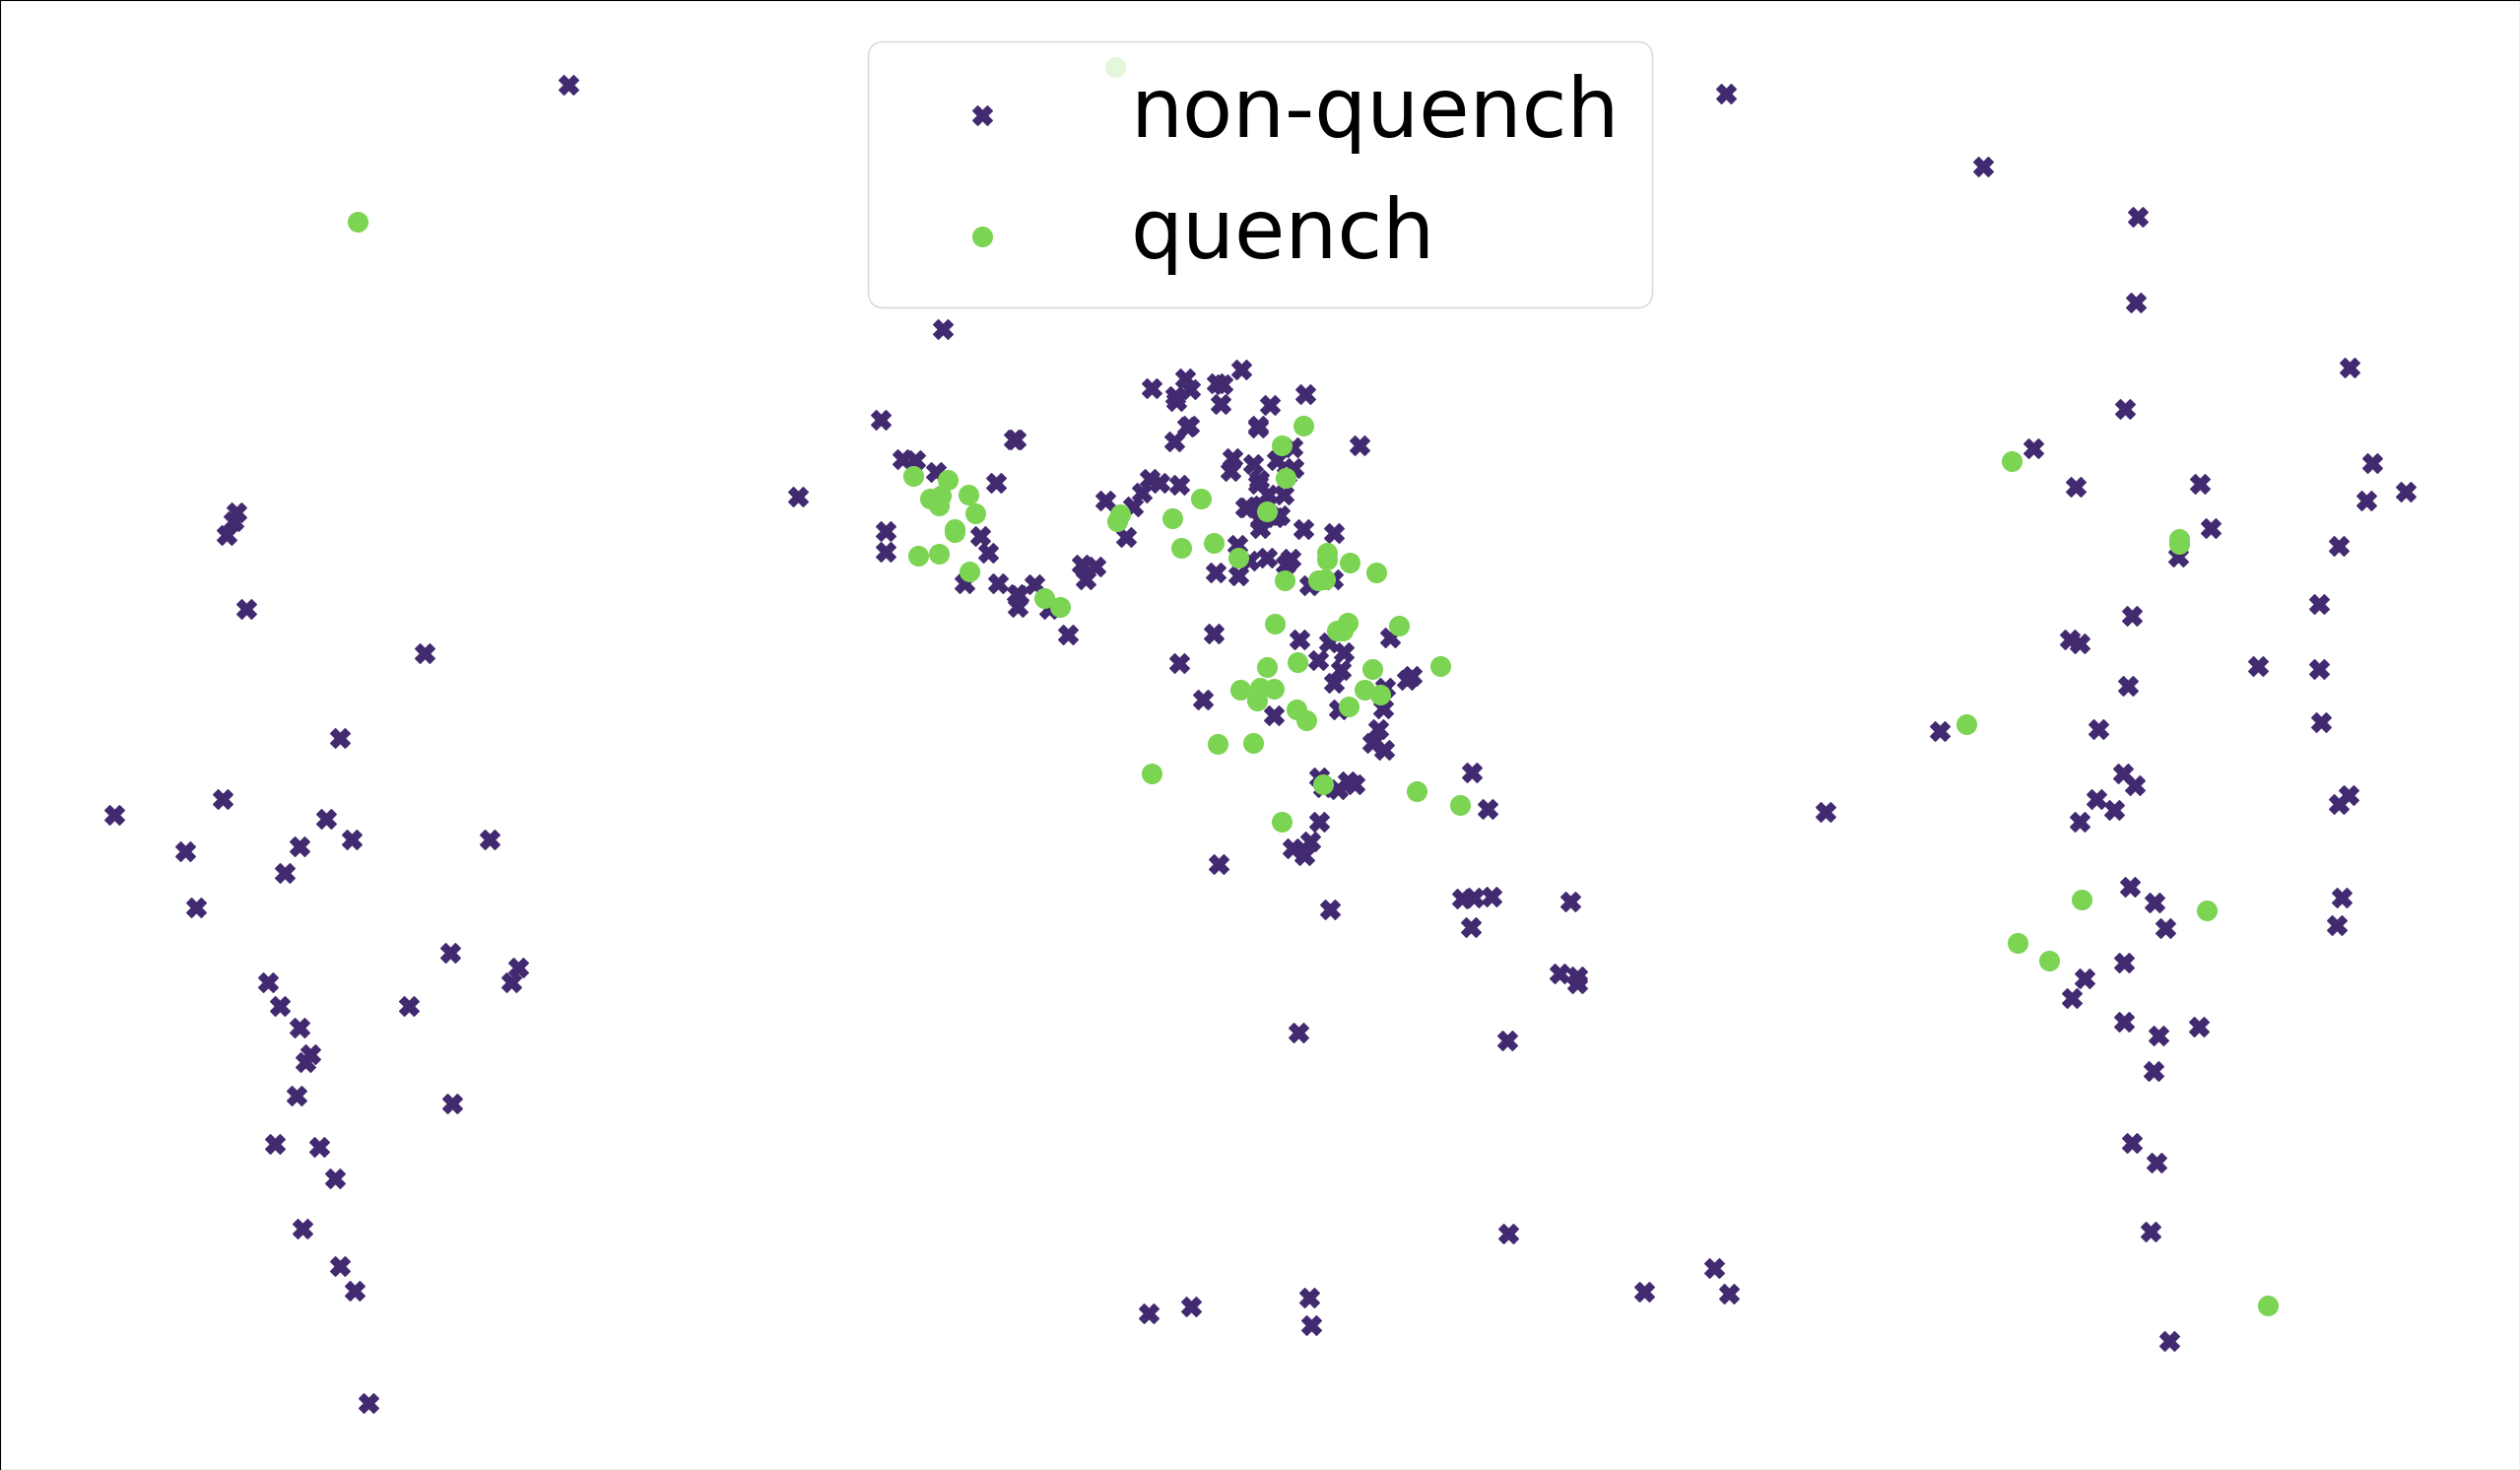
\includegraphics[width=\linewidth]{img/quench_dist_qlp/quenches_coil_0_Bn.png}
		\subcaption{}
	\end{subfigure}
	\begin{subfigure}{0.49\linewidth}
		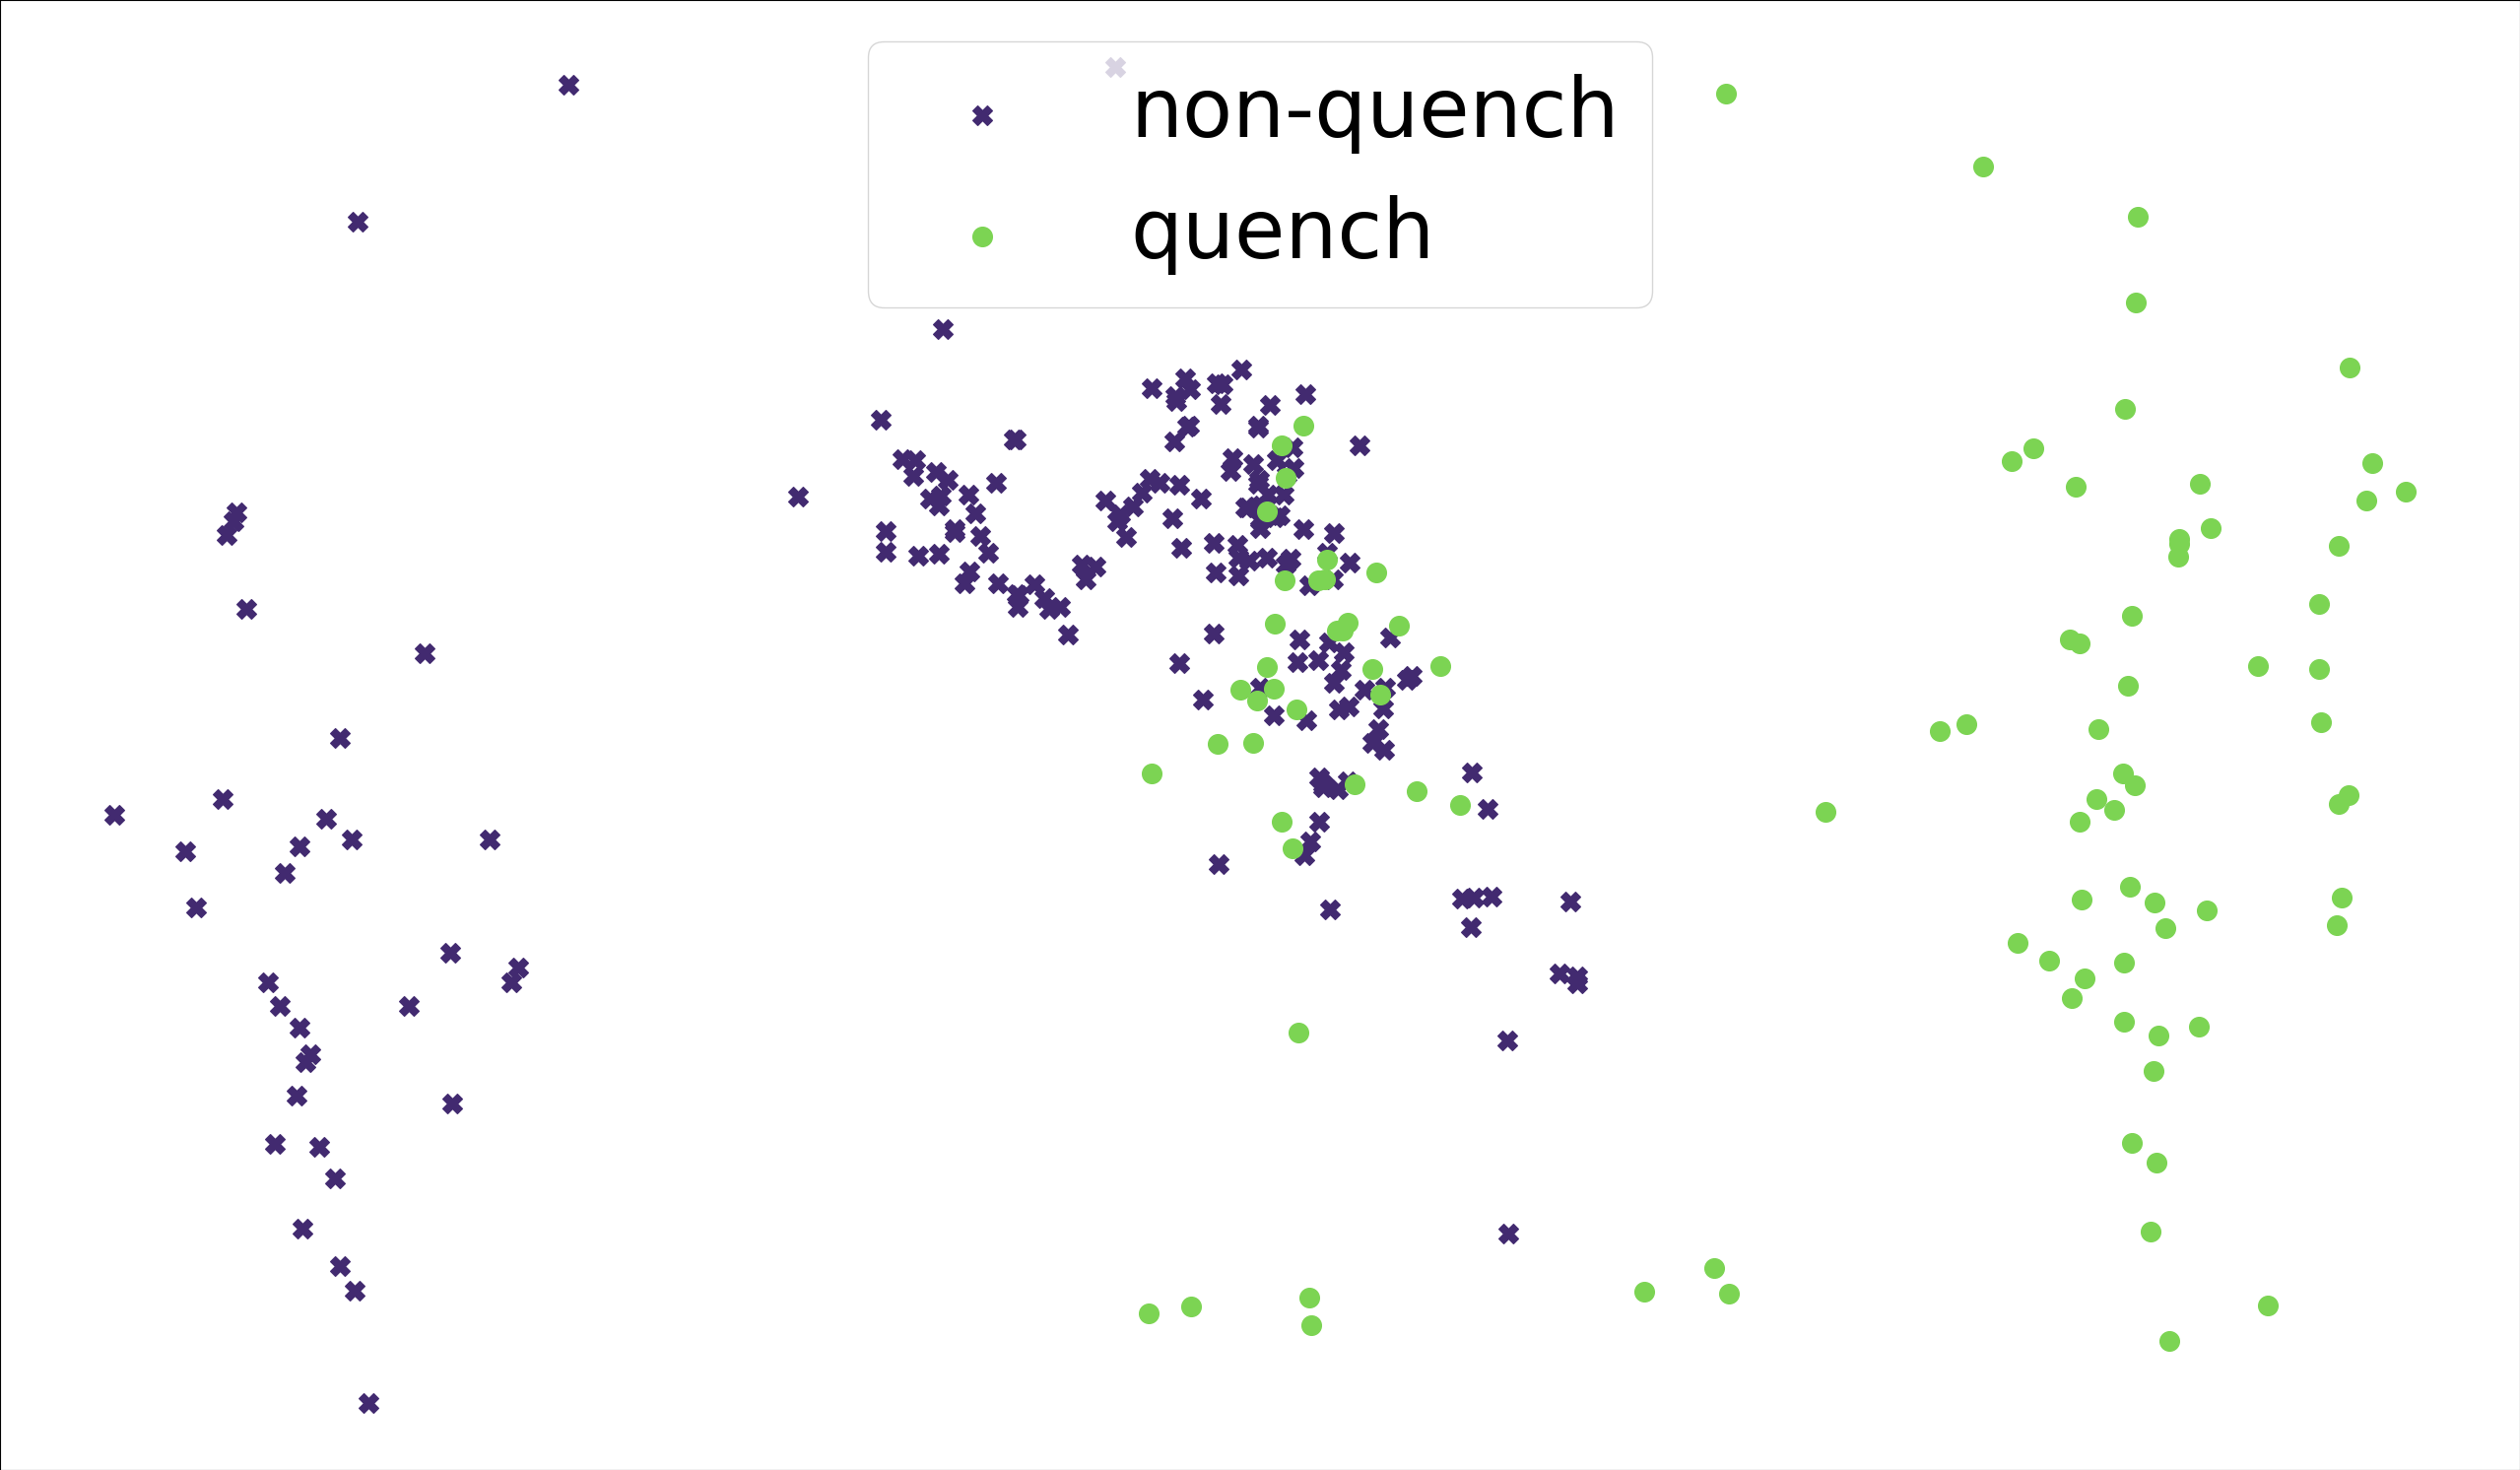
\includegraphics[width=\linewidth]{img/quench_dist_qlp/quenches_coil_1_Bn.png}
		\subcaption{}
	\end{subfigure}
	\begin{subfigure}{0.49\linewidth}
		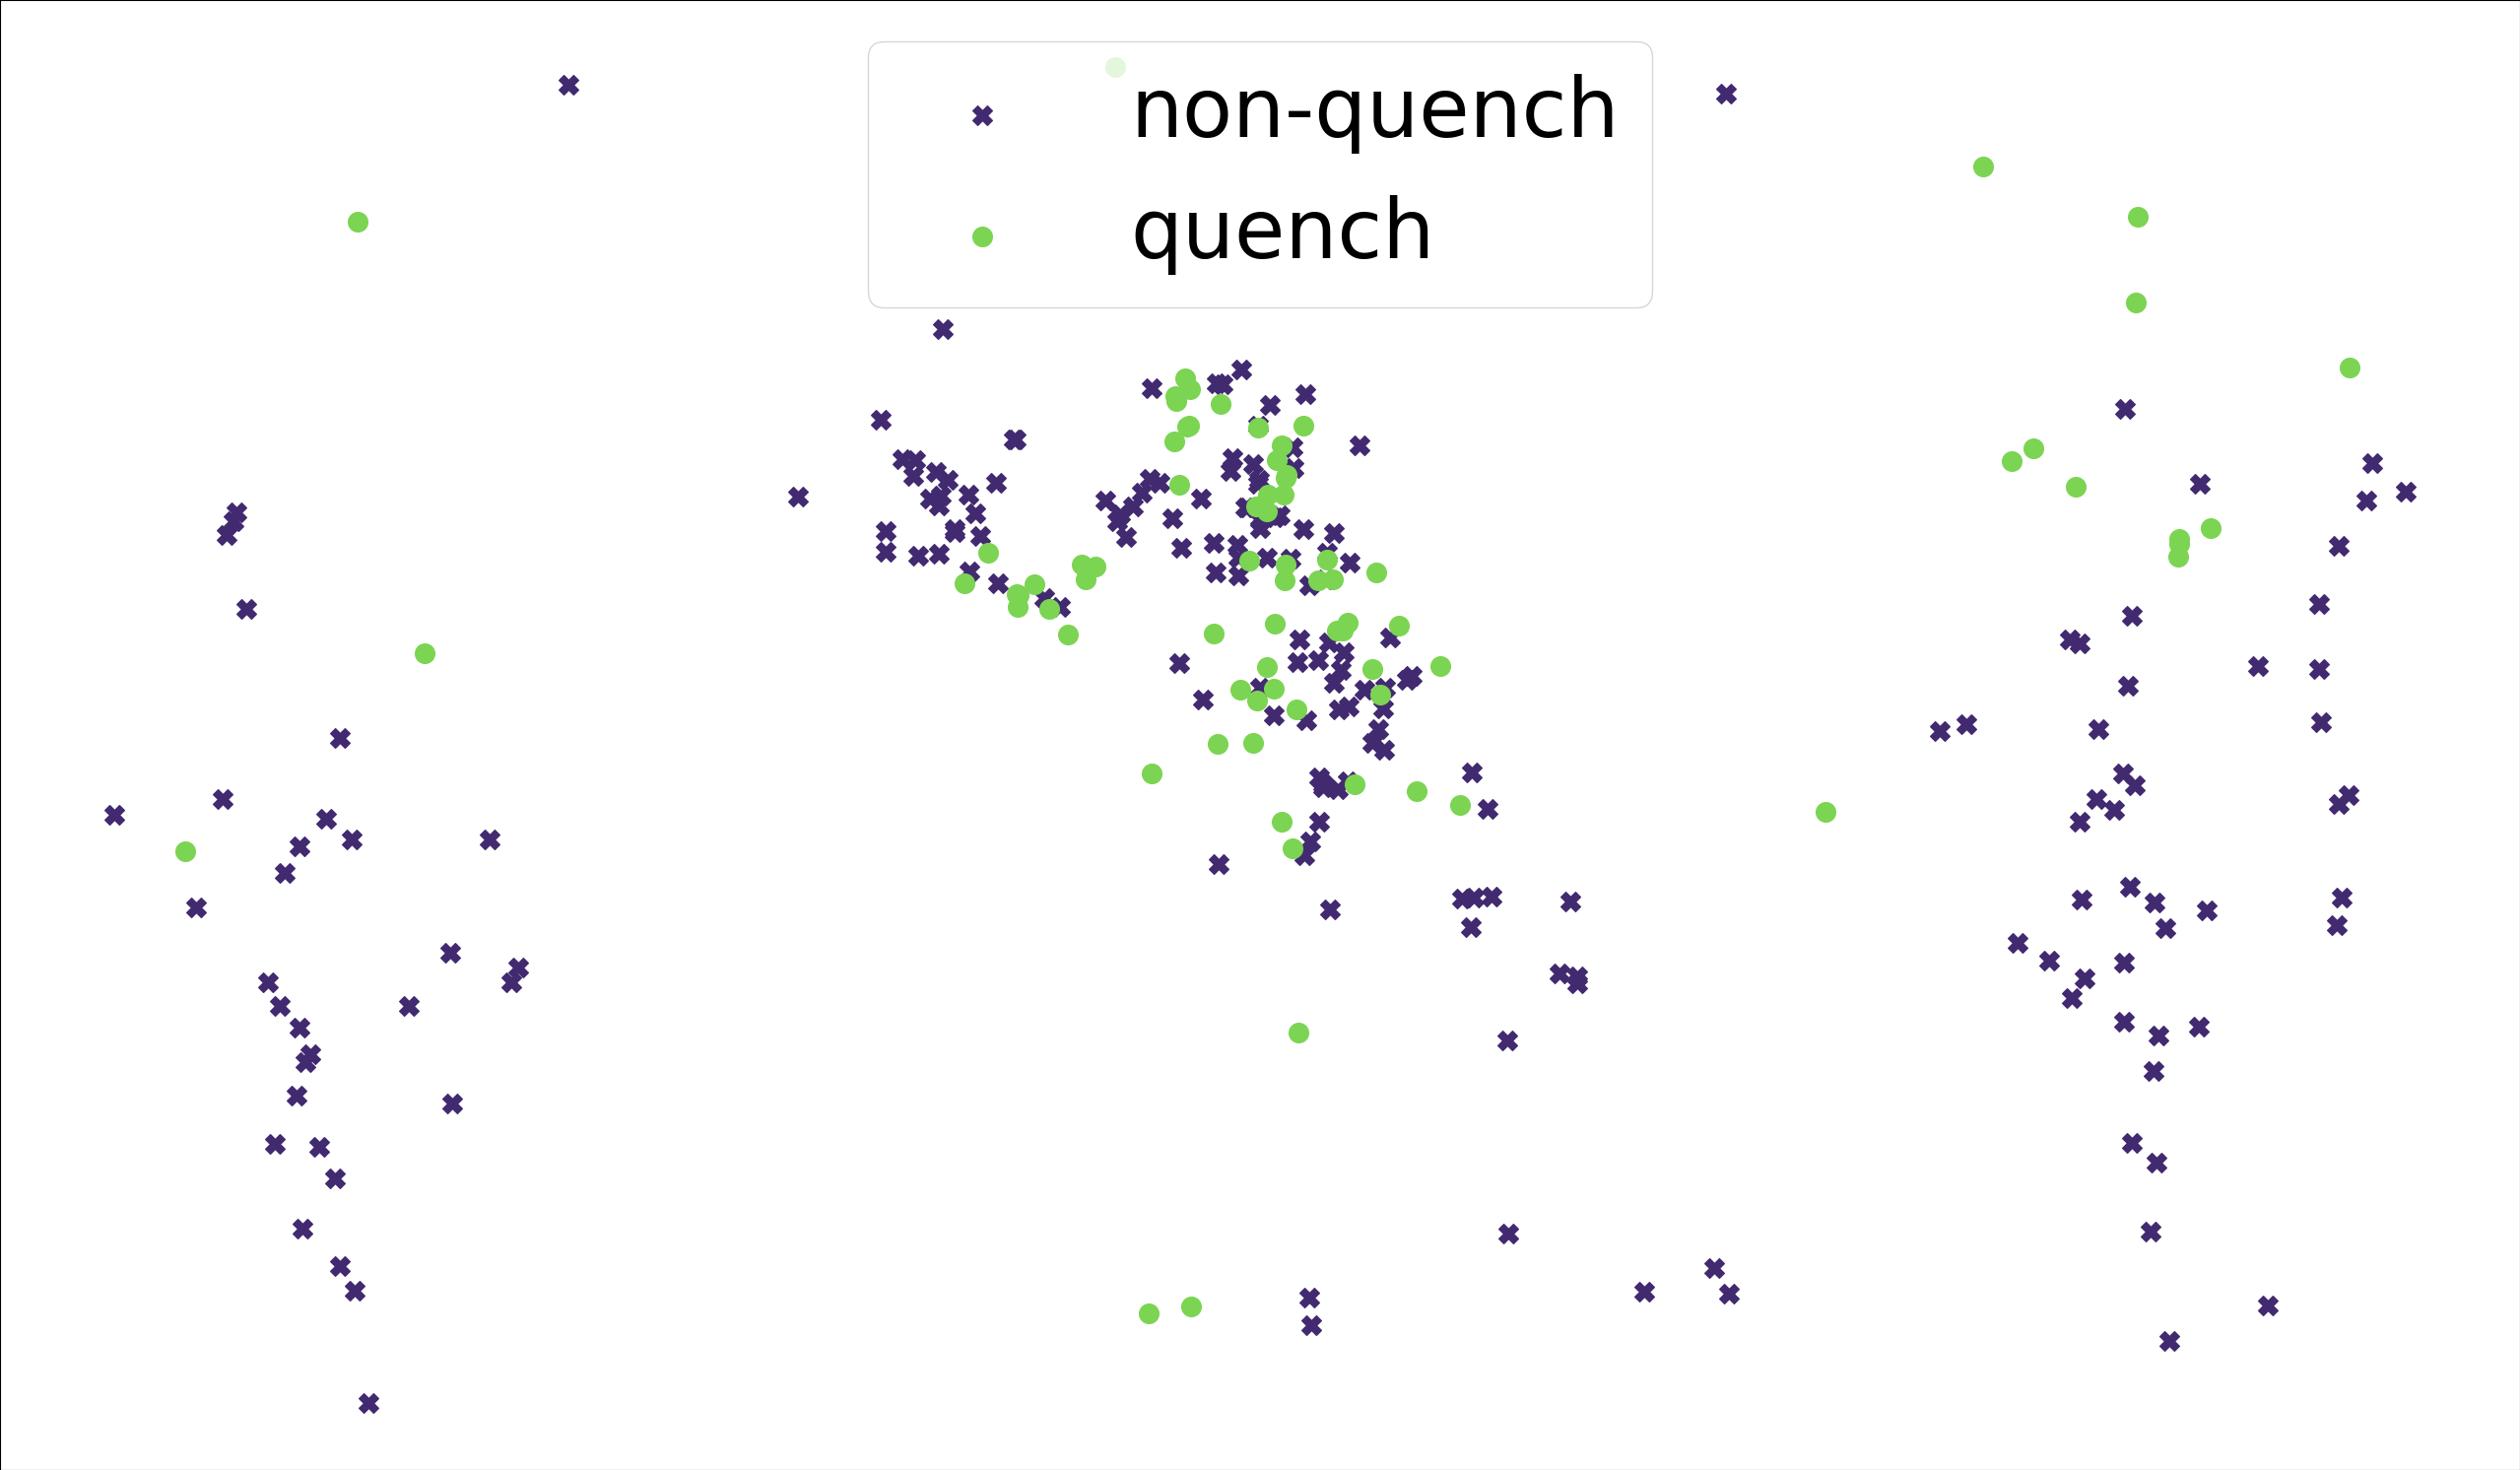
\includegraphics[width=\linewidth]{img/quench_dist_qlp/quenches_coil_2_Bn.png}
		\subcaption{}
	\end{subfigure}
	\begin{subfigure}{0.49\linewidth}
		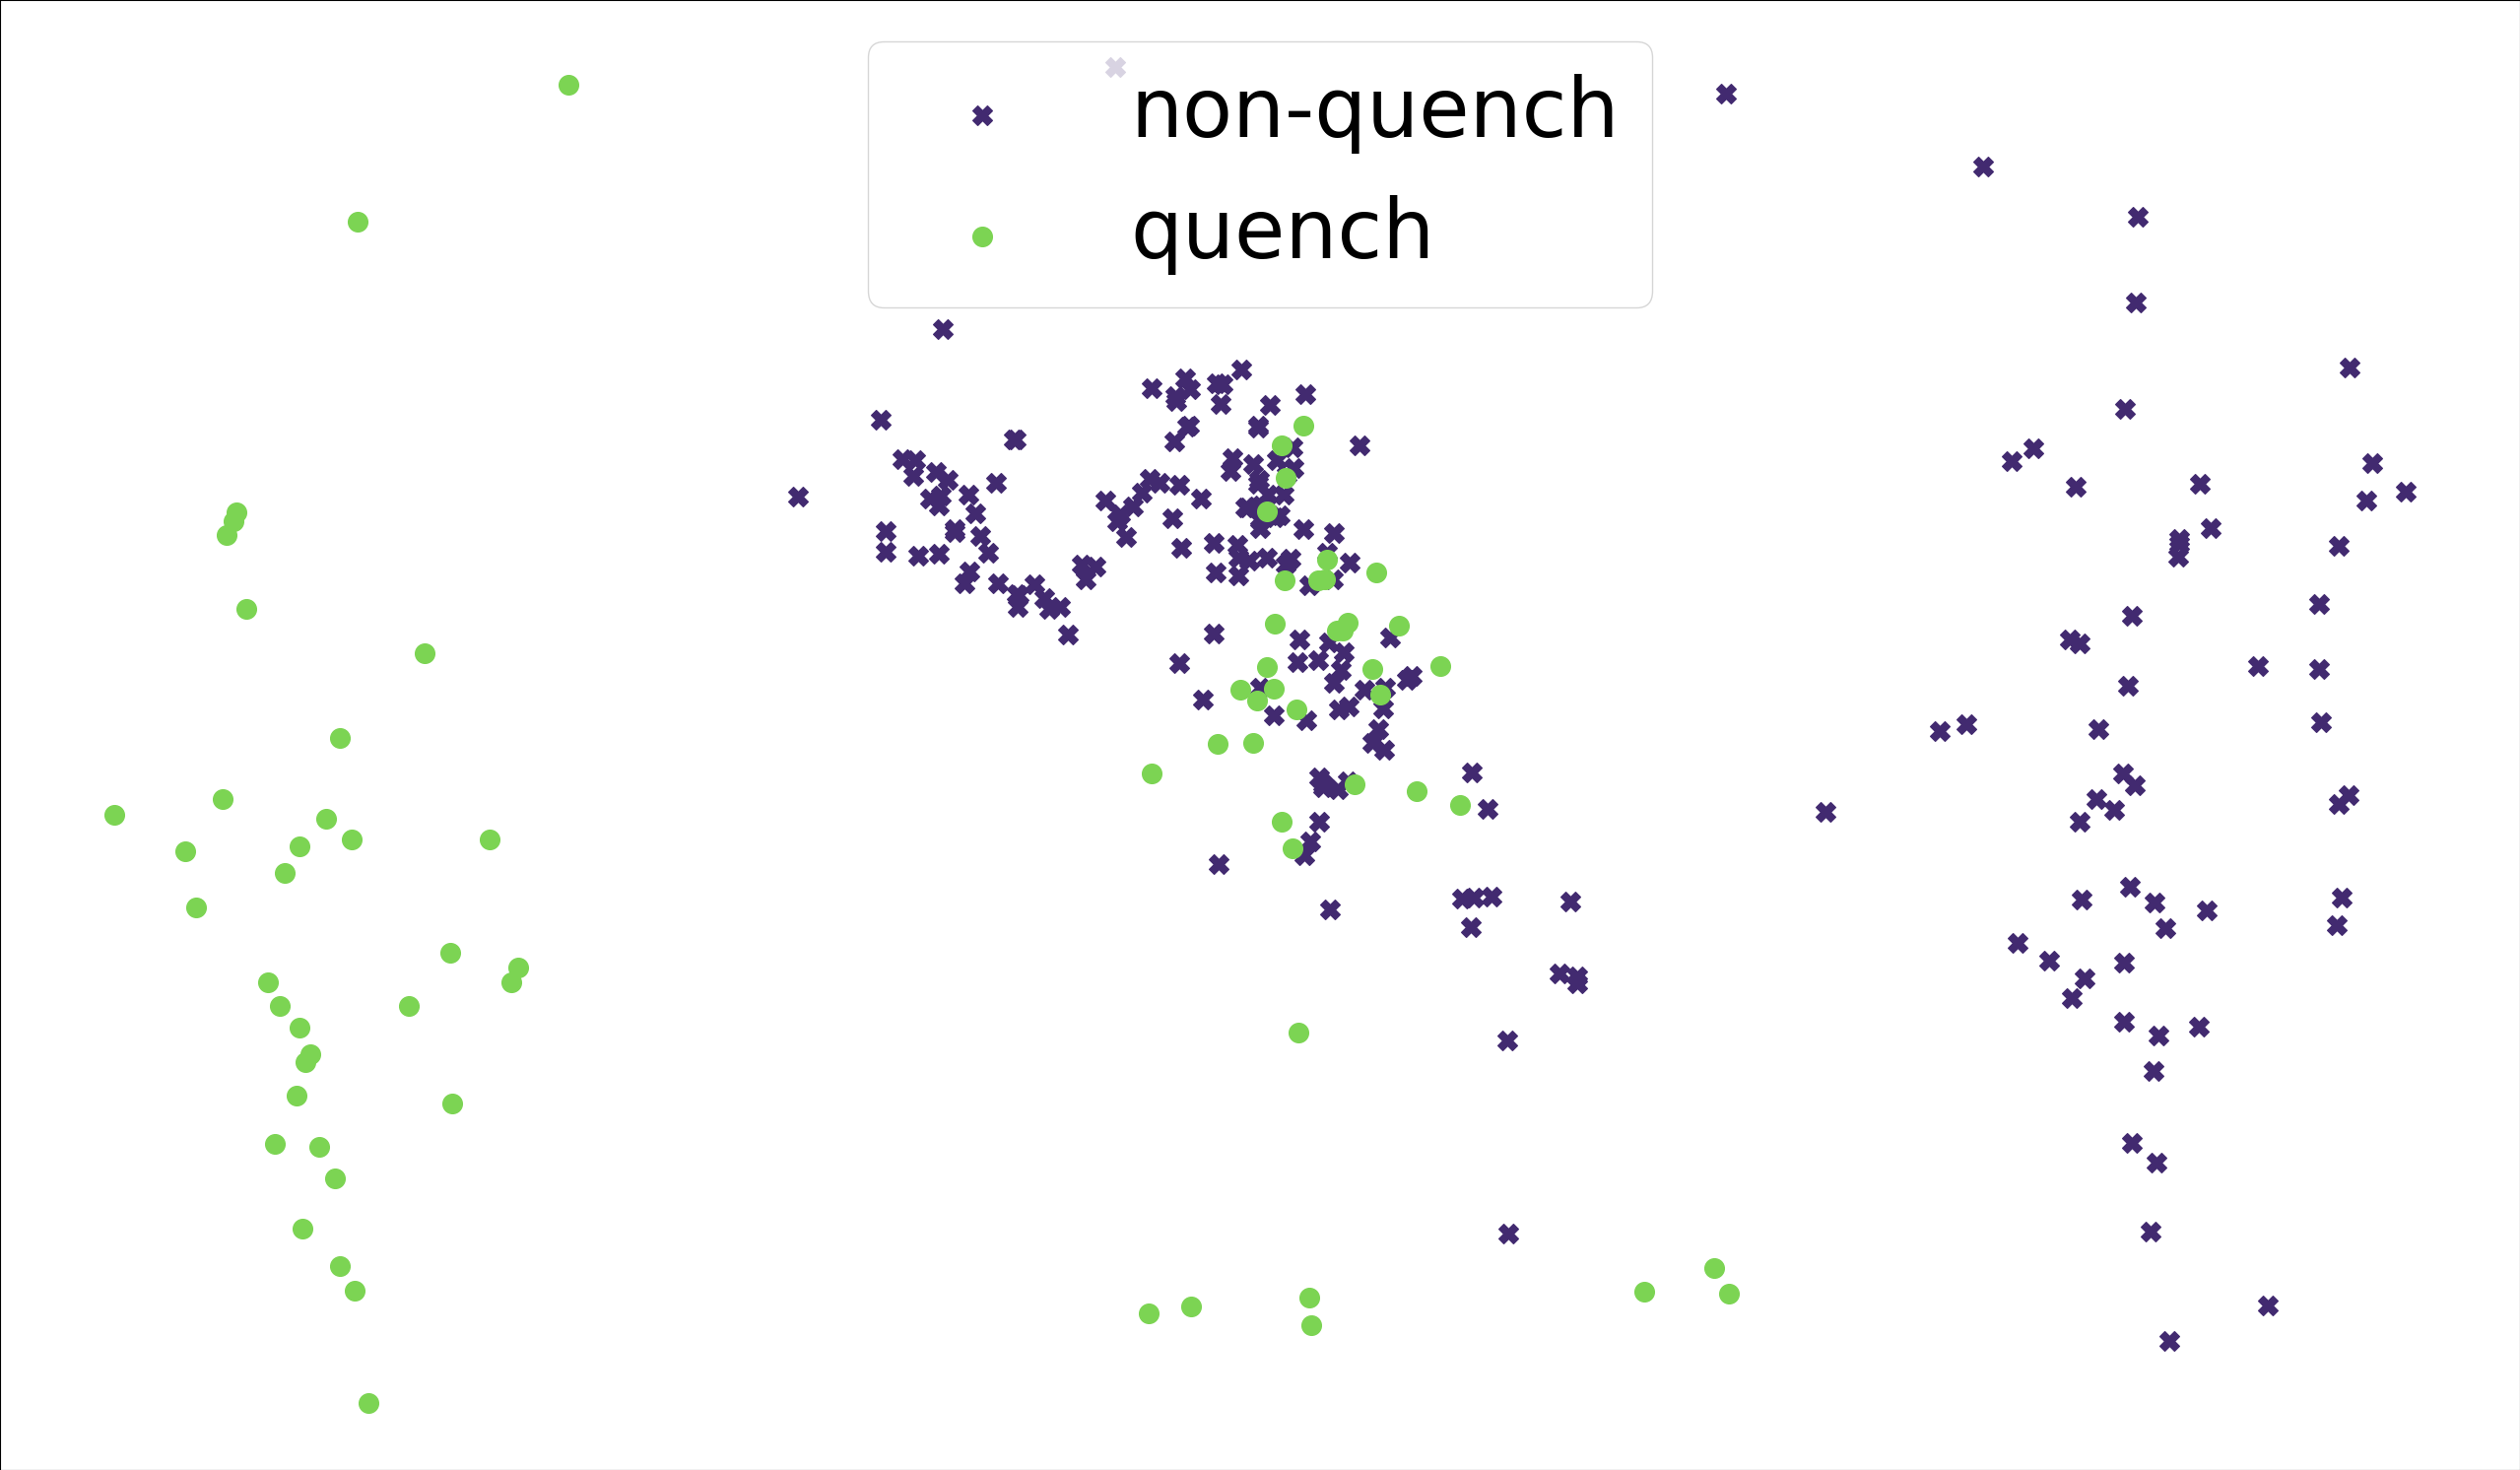
\includegraphics[width=\linewidth]{img/quench_dist_qlp/quenches_coil_3_Bn.png}
		\subcaption{}
	\end{subfigure}
	\caption{The distribution of the samples in bidimensional space after a round of \pca, for
		the \an\ attribute. the subfigures contain different views of the same data: (a) differenciates between non-quench and single or multiple quench events, (b) highlights the distribution of quenches for coil $0$, (c) highlights the distribution of quenches for coil $1$, (d) highlights the distribution of quenches for coil $2$ and finally (e) highlights the distribution of quenches for coil $3$.}
	\label{fig:bn-coilq-dist}
\end{figure}

\subsubsection{\cnmod}
The \cnmod attribute, while highly informative for \qrp, we expected \cnmod\ to be a valuable feature for \qrp\
and not for \qlp\ since (in the original experiment, described in \Cref{chp:problem}) two different
configurations with the same number of quenched coils, but different angular positions, would give
the same harmonic content and different phases. If we analyze the correlation between the harmonics
and the labels (see \Cref{fig:cnmod-lcorr-qlp}), we have a structure similar to the one highlighted dor \an\ and \bn, but it's
shifted forward by one (e.g., instead of having harmonics $3, 4$ and $5$ strongly correlated with
the labels, we have $5, 6$ and $7$). Furthermore \cnmod\ seems to be highly correlated with coil
$3$.

If we look back at the correlation matrix computed for \cnmod\ during the preprocessing for \qrp\
(see \Cref{fig:cnmod-corr}) we could say that the structure of a sub-view of \cnmod\ could be built:
\begin{itemize}
	\item in the case of coil $0$, starting from harmonic $2$ and adding a high-order candidate.
	      While this would technically maximize the total correlation with the label we have
	      seen in \qrp\ that choosing harmonic number $2$ was a choice that didn't pay. That
	      is why we should be using harmonics number $3$ alongside harmonic number $6$ and
	      another high order harmonics like $9, 11$.
	\item in the case of coil $3$, we could be taking harmonic $1$ and then using one or more from $4,
		      5, 6, 7$ and $8$ and finally, if it makes performance better, we could also add
	      another high order harmonic like $10$.
\end{itemize}

\begin{figure}[!h]
	% Font size = 70
	\centering
	\begin{subfigure}{0.49\linewidth}
		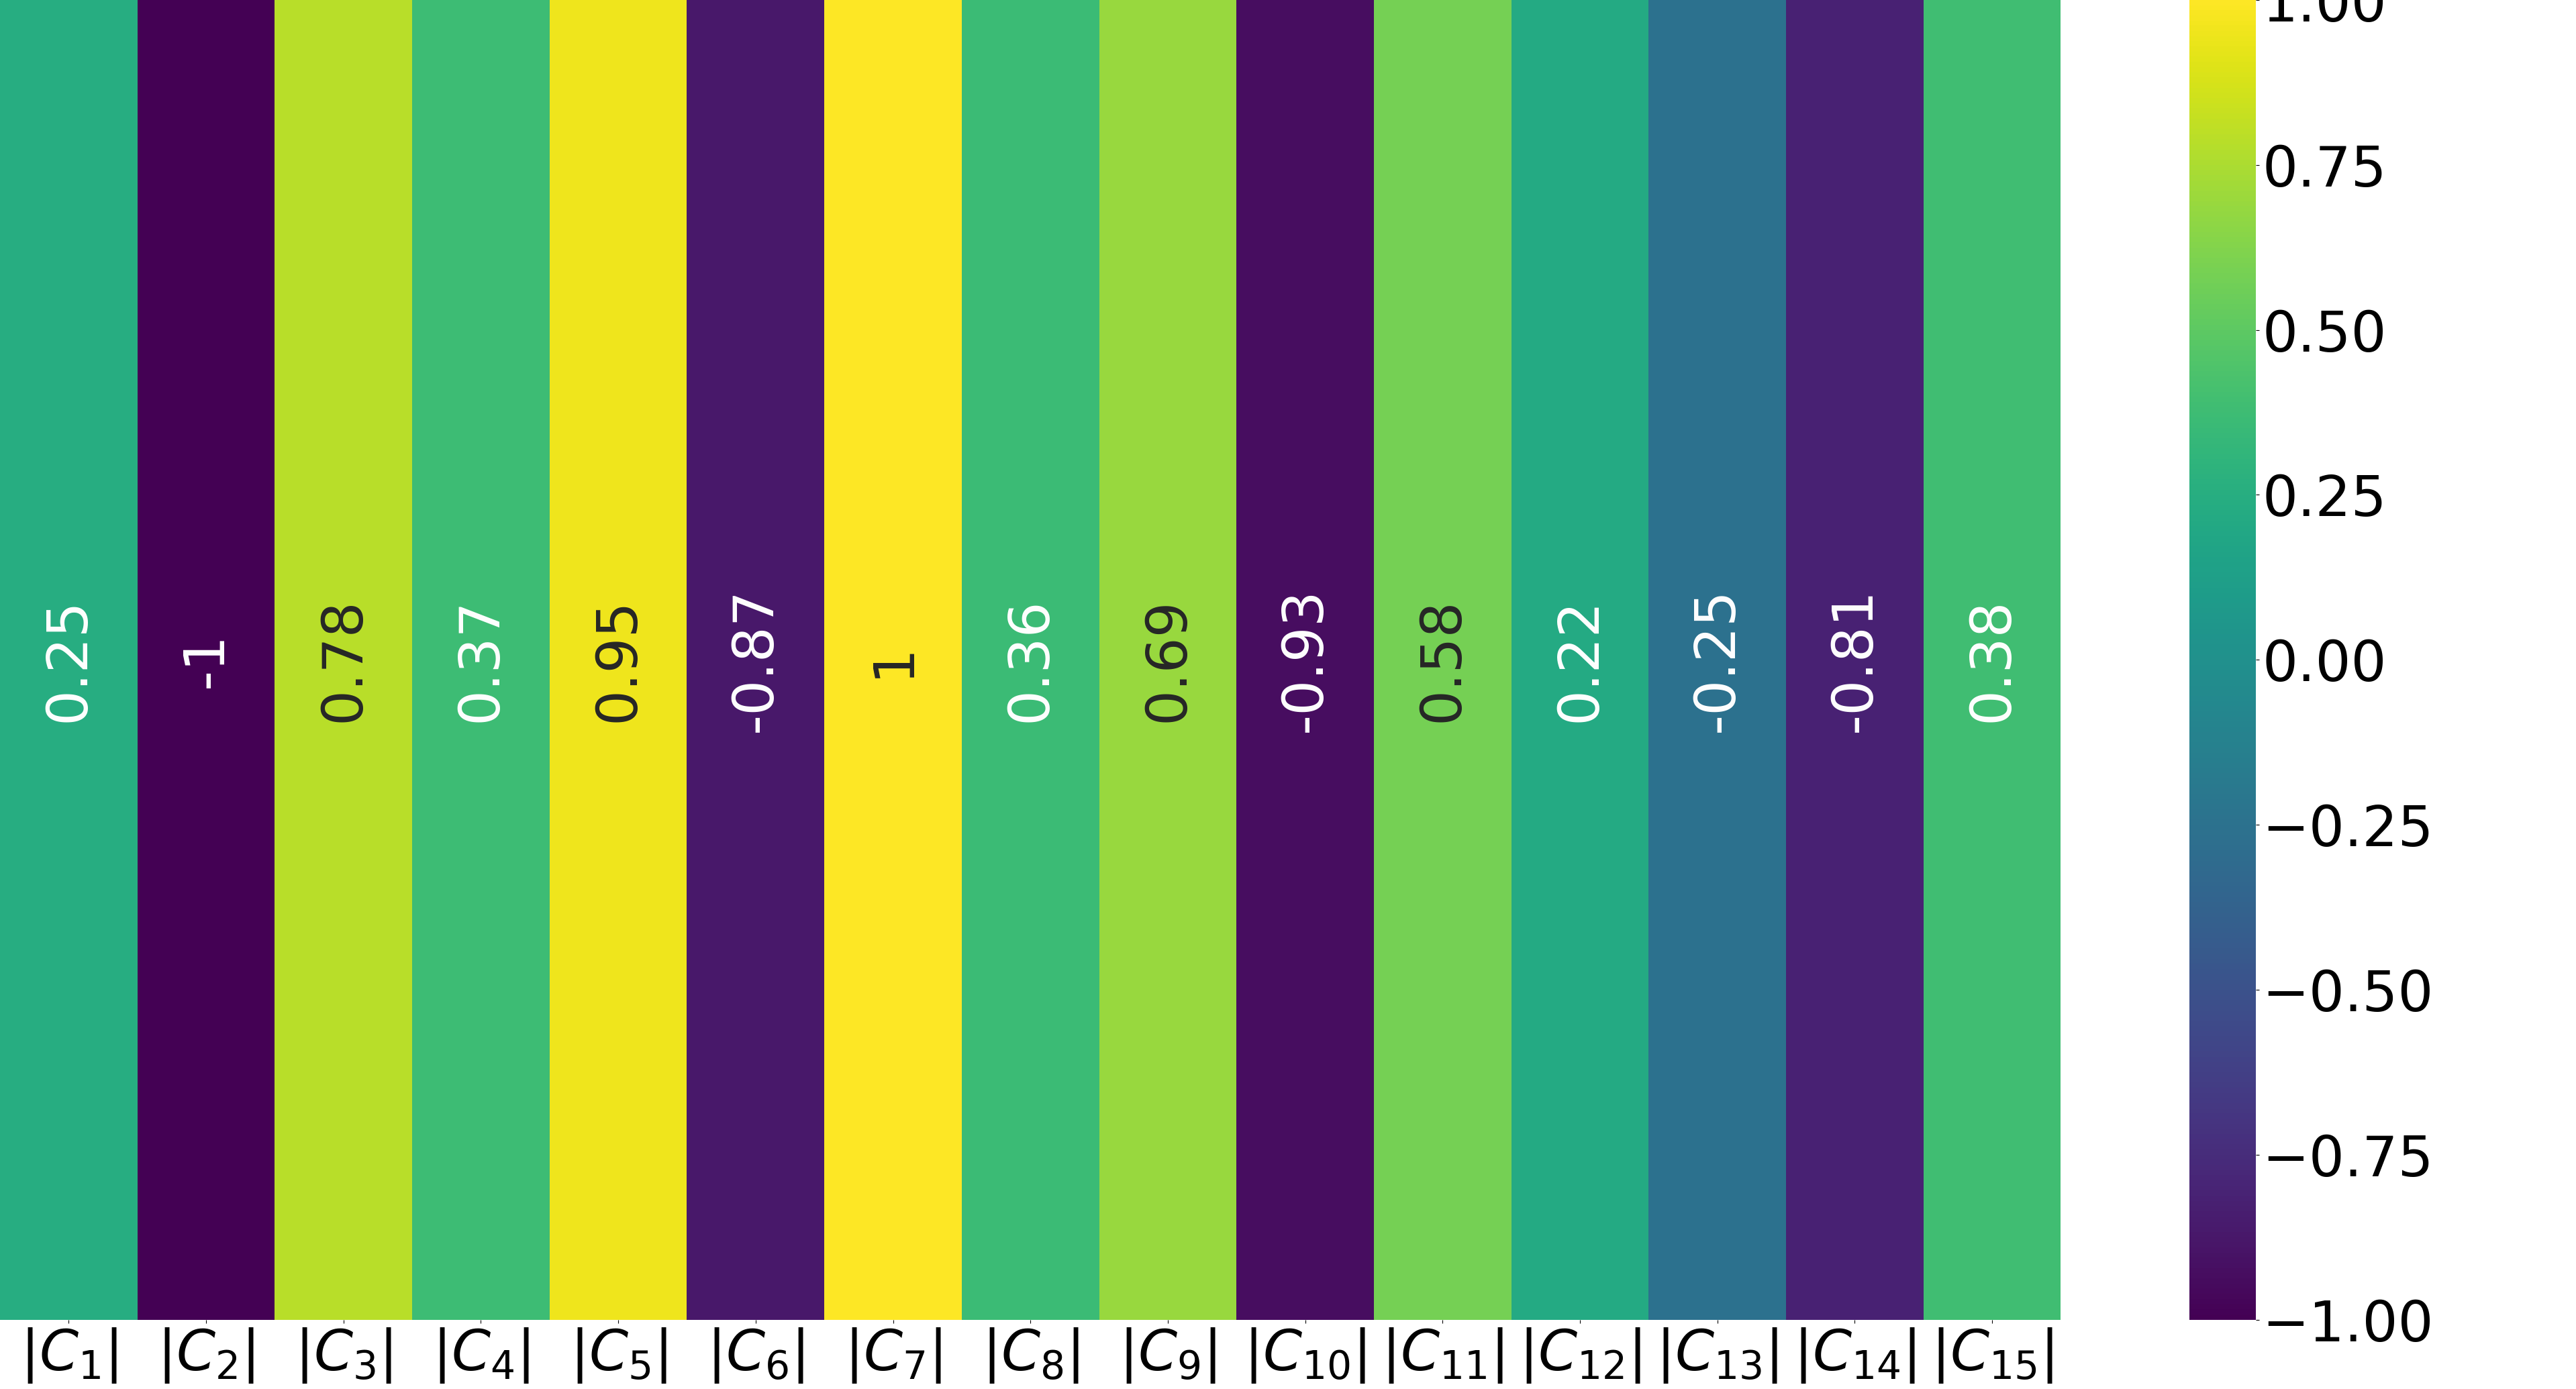
\includegraphics[width=\linewidth]{img/qlp_corr/Cnmod_coil0.png}
		\subcaption{Correlation with coil $0$}
	\end{subfigure}
	\begin{subfigure}{0.49\linewidth}
		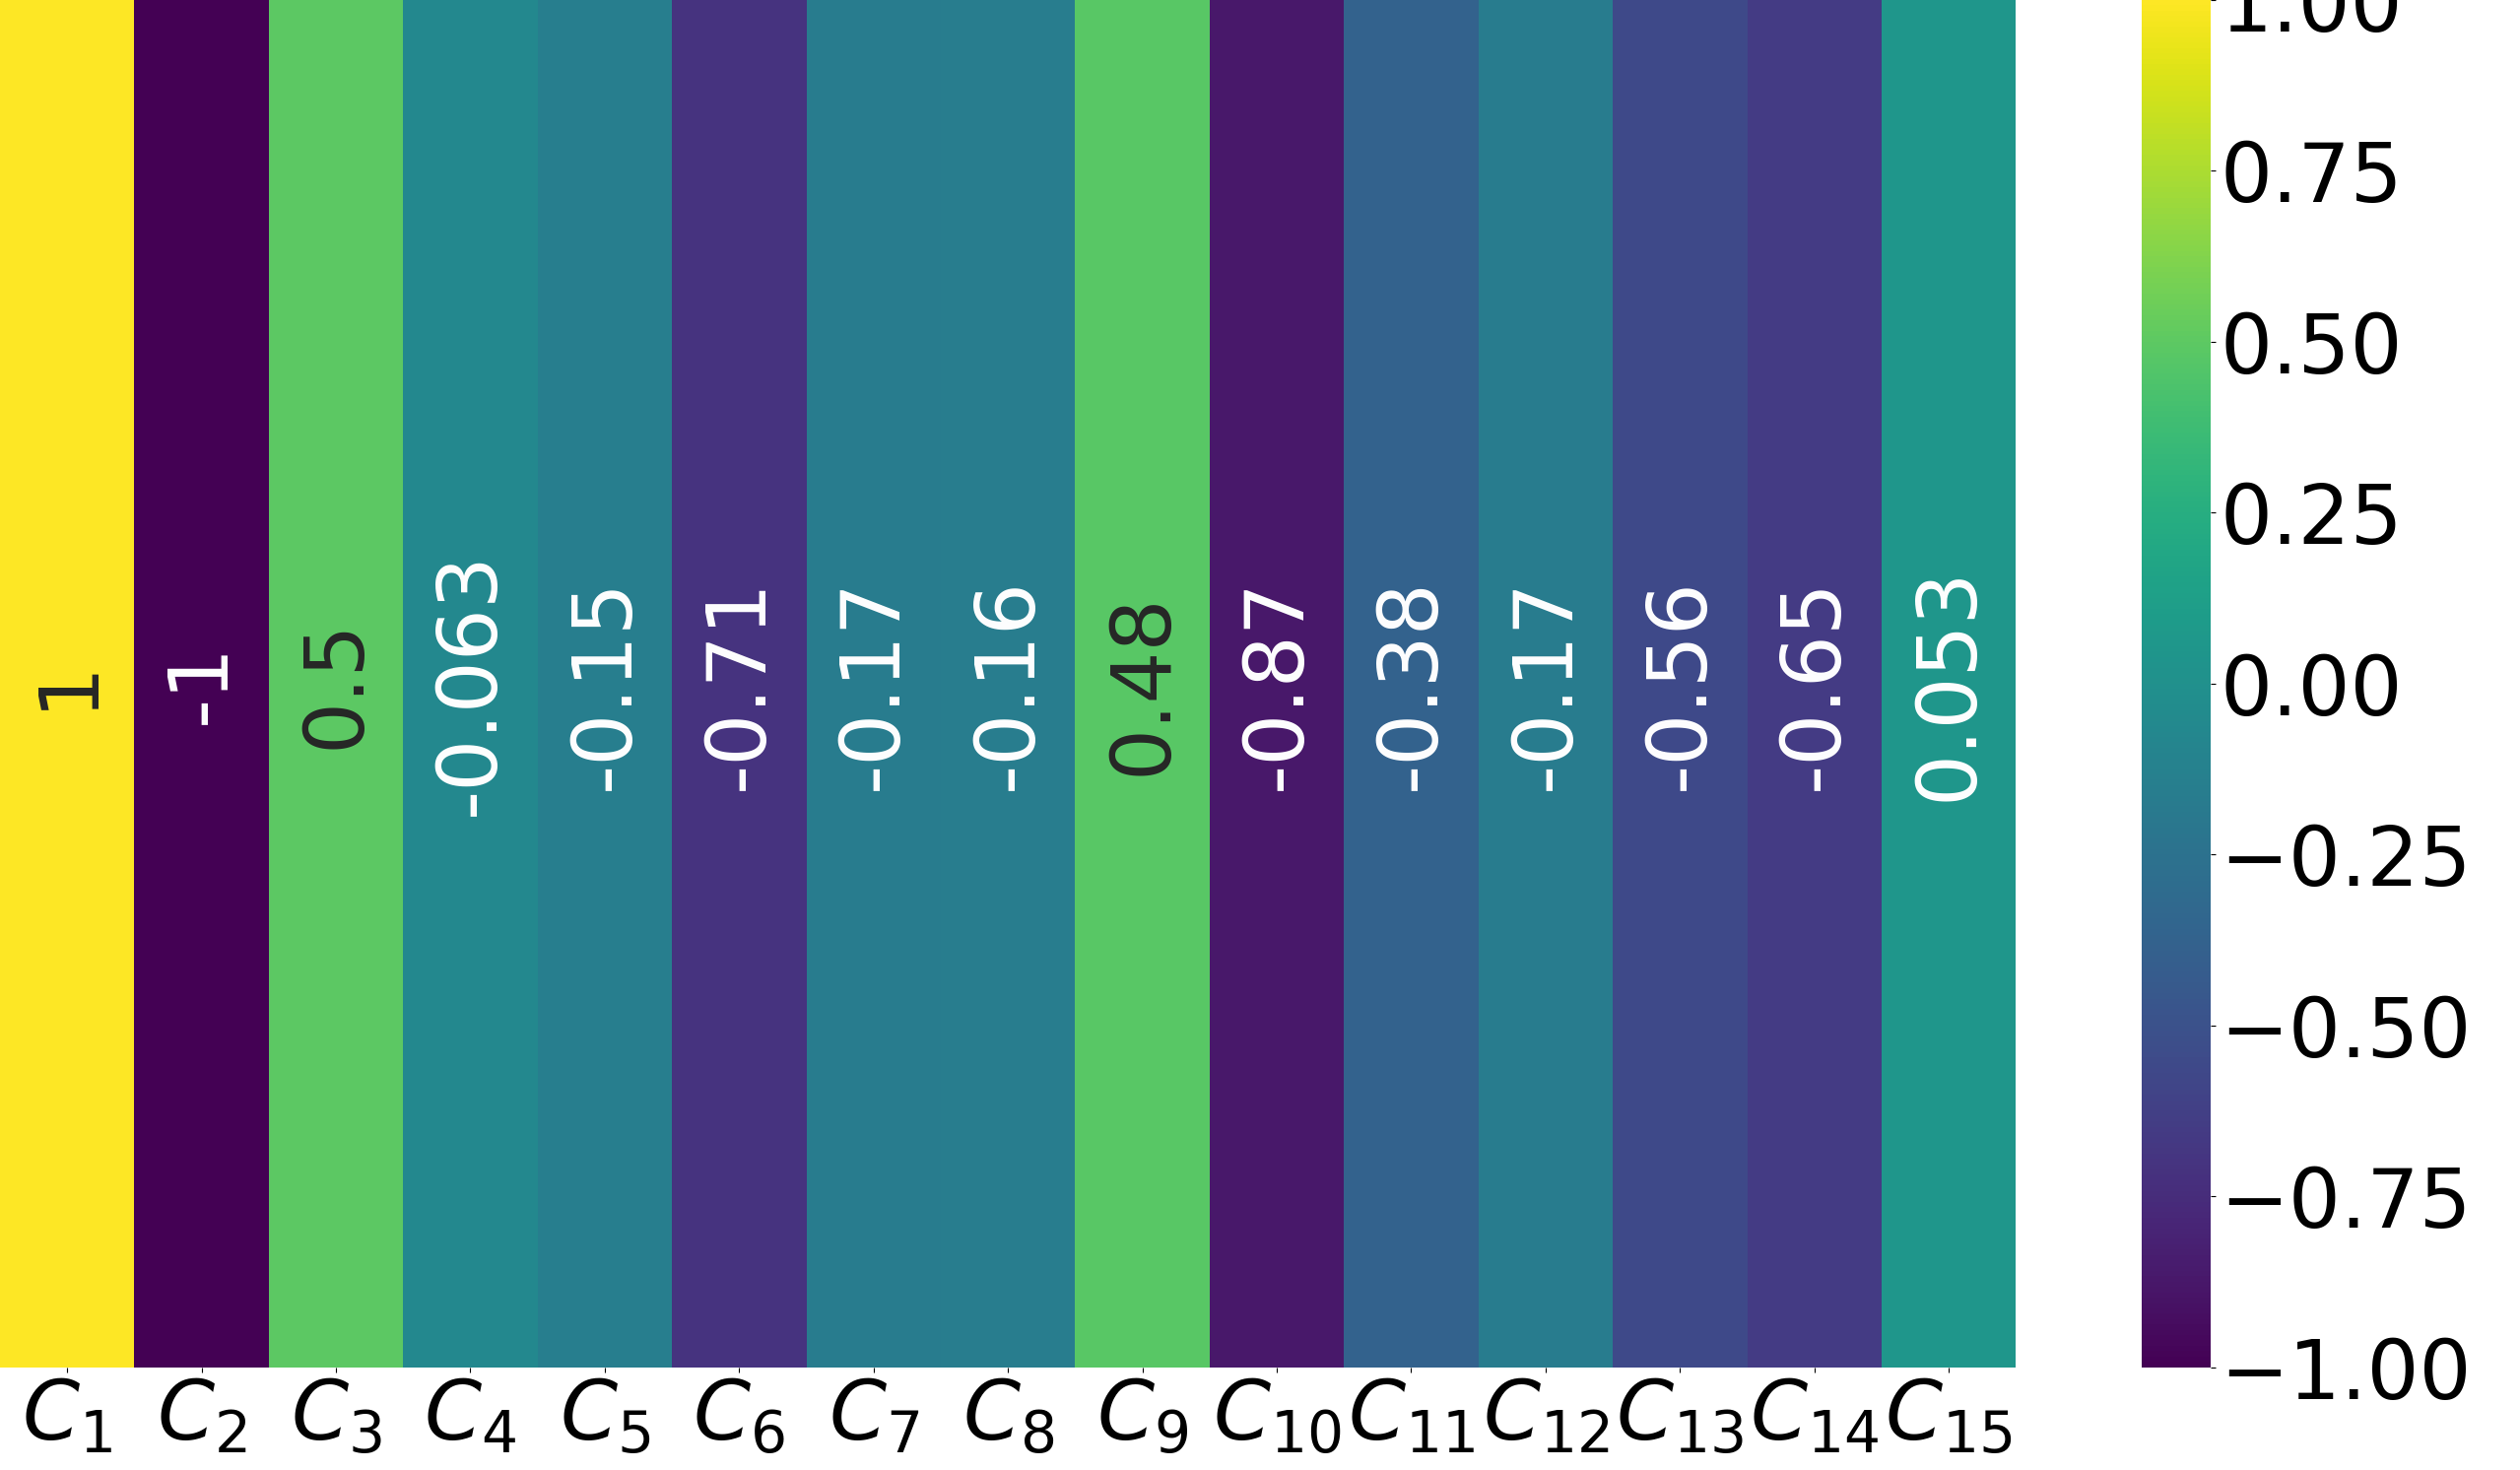
\includegraphics[width=\linewidth]{img/qlp_corr/Cnmod_coil1.png}
		\subcaption{Correlation with coil $1$}
	\end{subfigure}
	\begin{subfigure}{0.49\linewidth}
		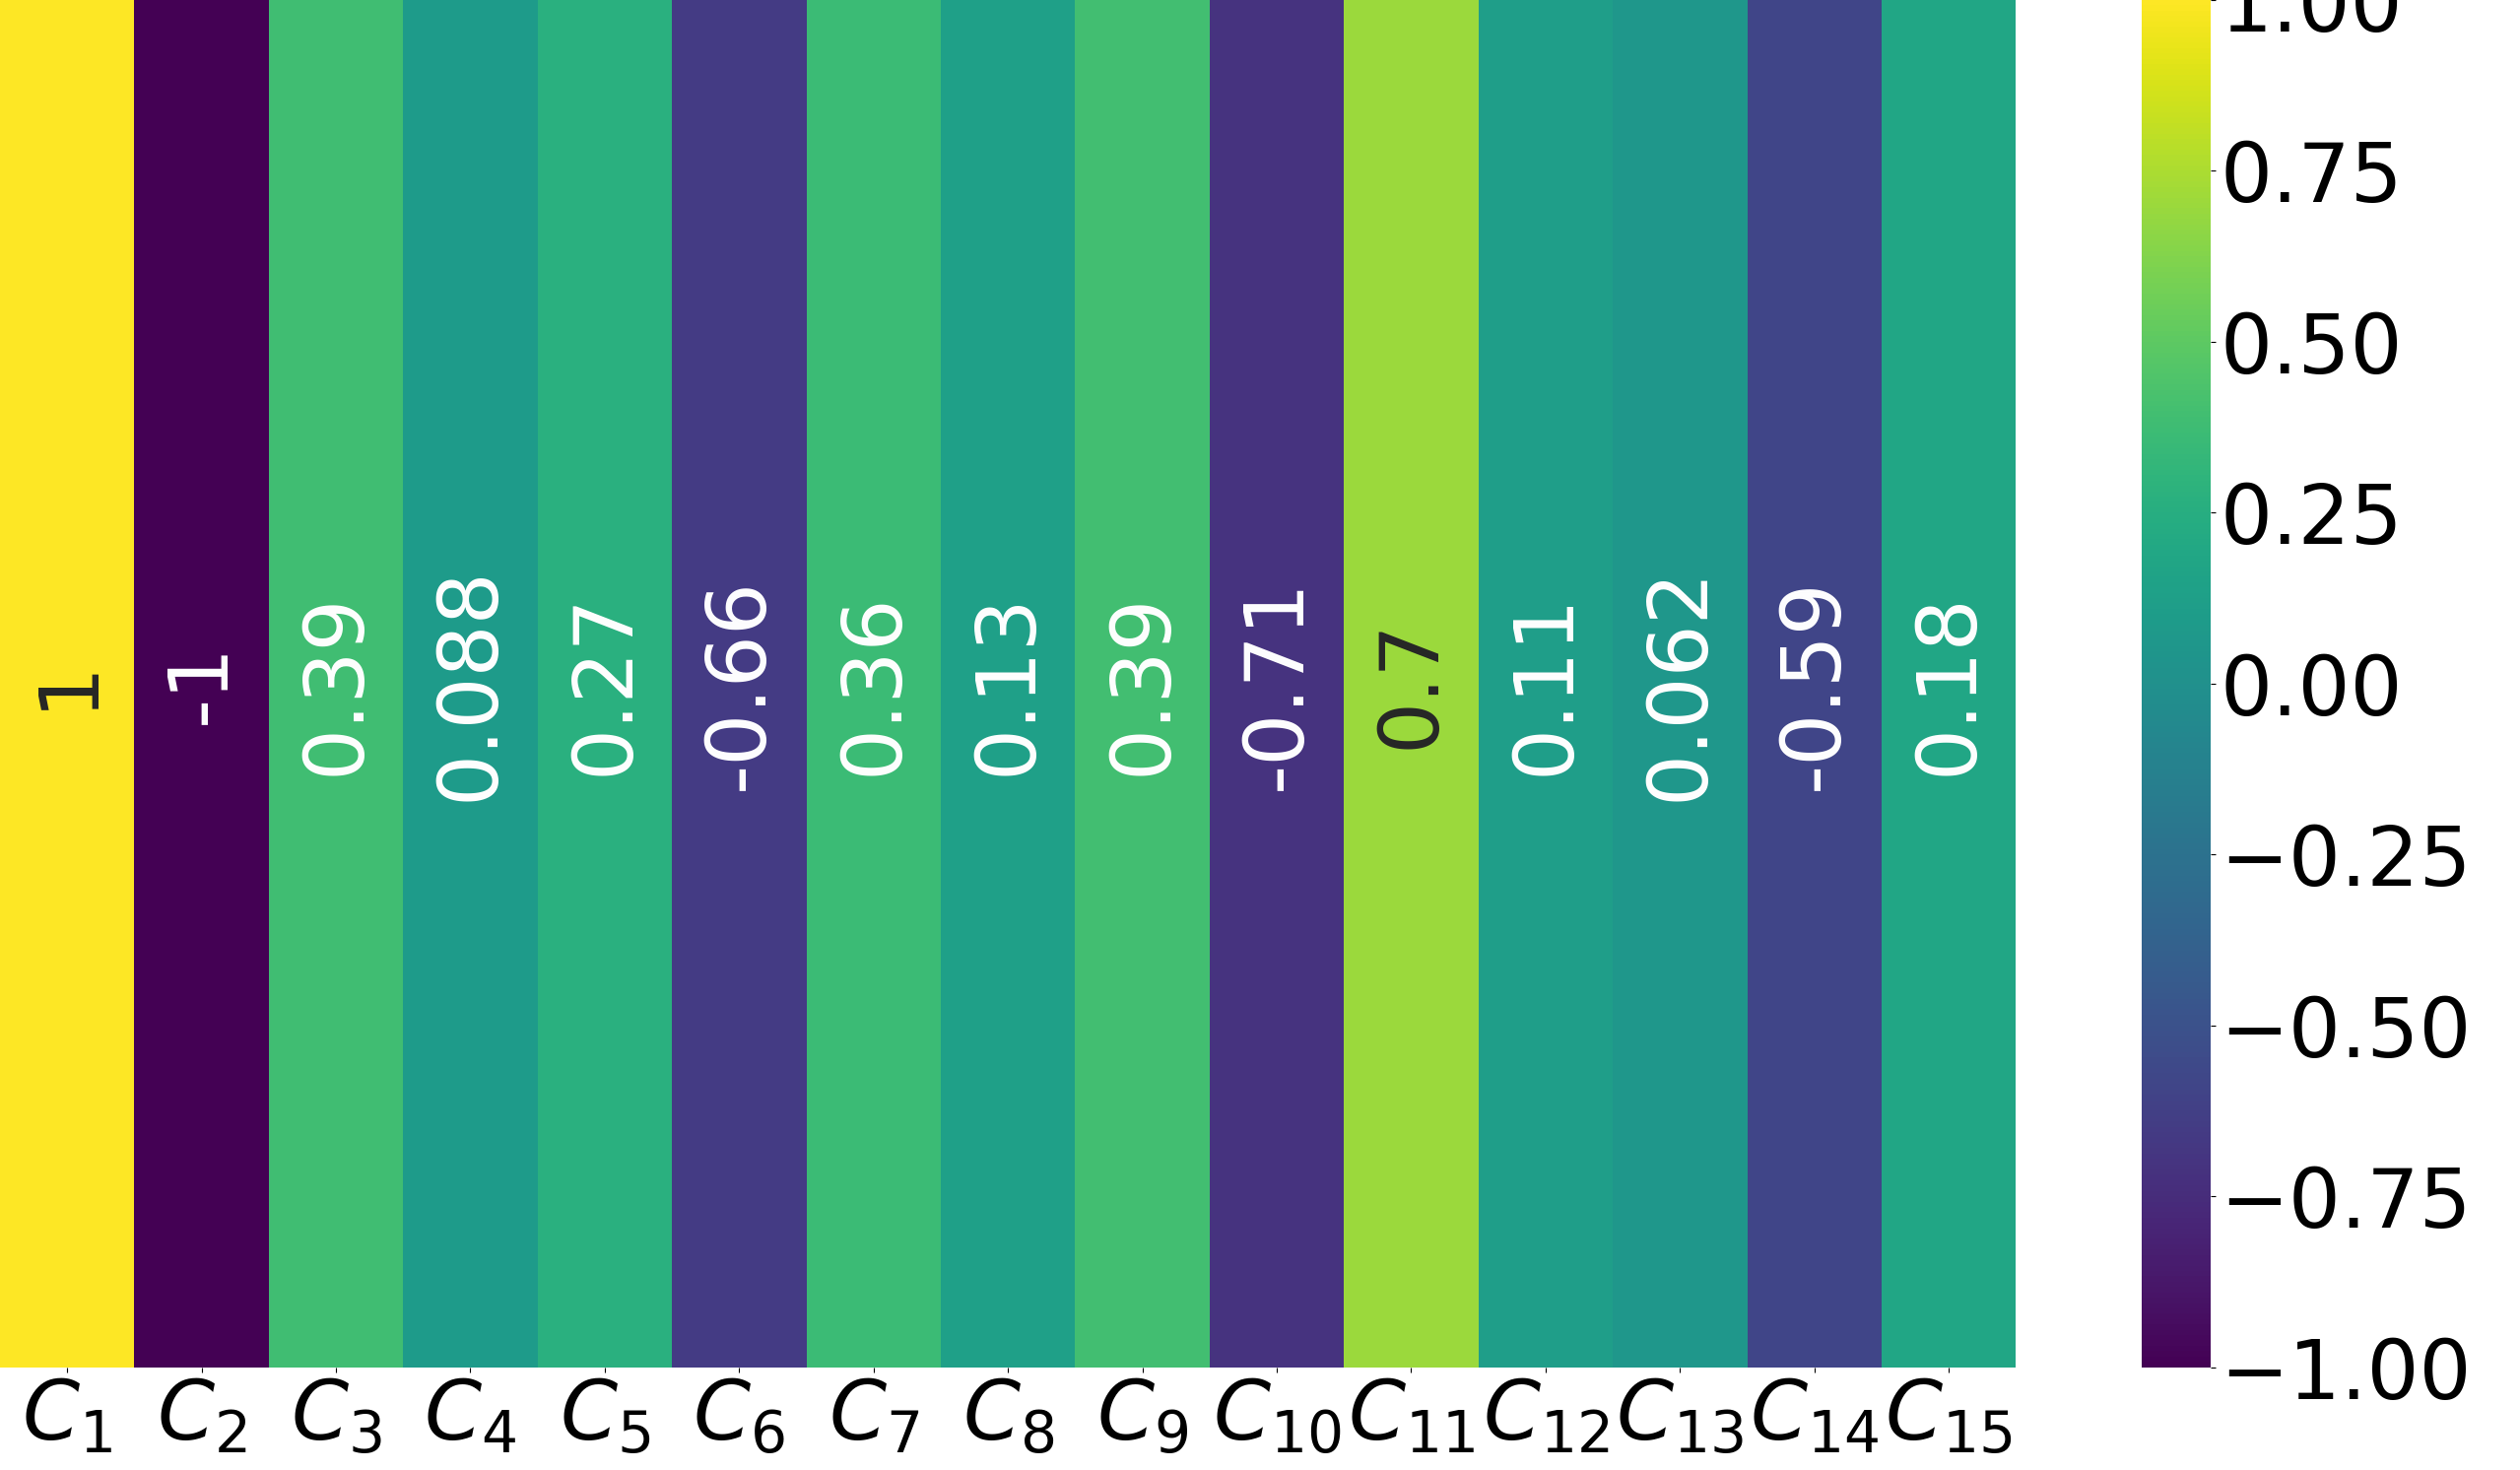
\includegraphics[width=\linewidth]{img/qlp_corr/Cnmod_coil2.png}
		\subcaption{Correlation with coil $2$}
	\end{subfigure}
	\begin{subfigure}{0.49\linewidth}
		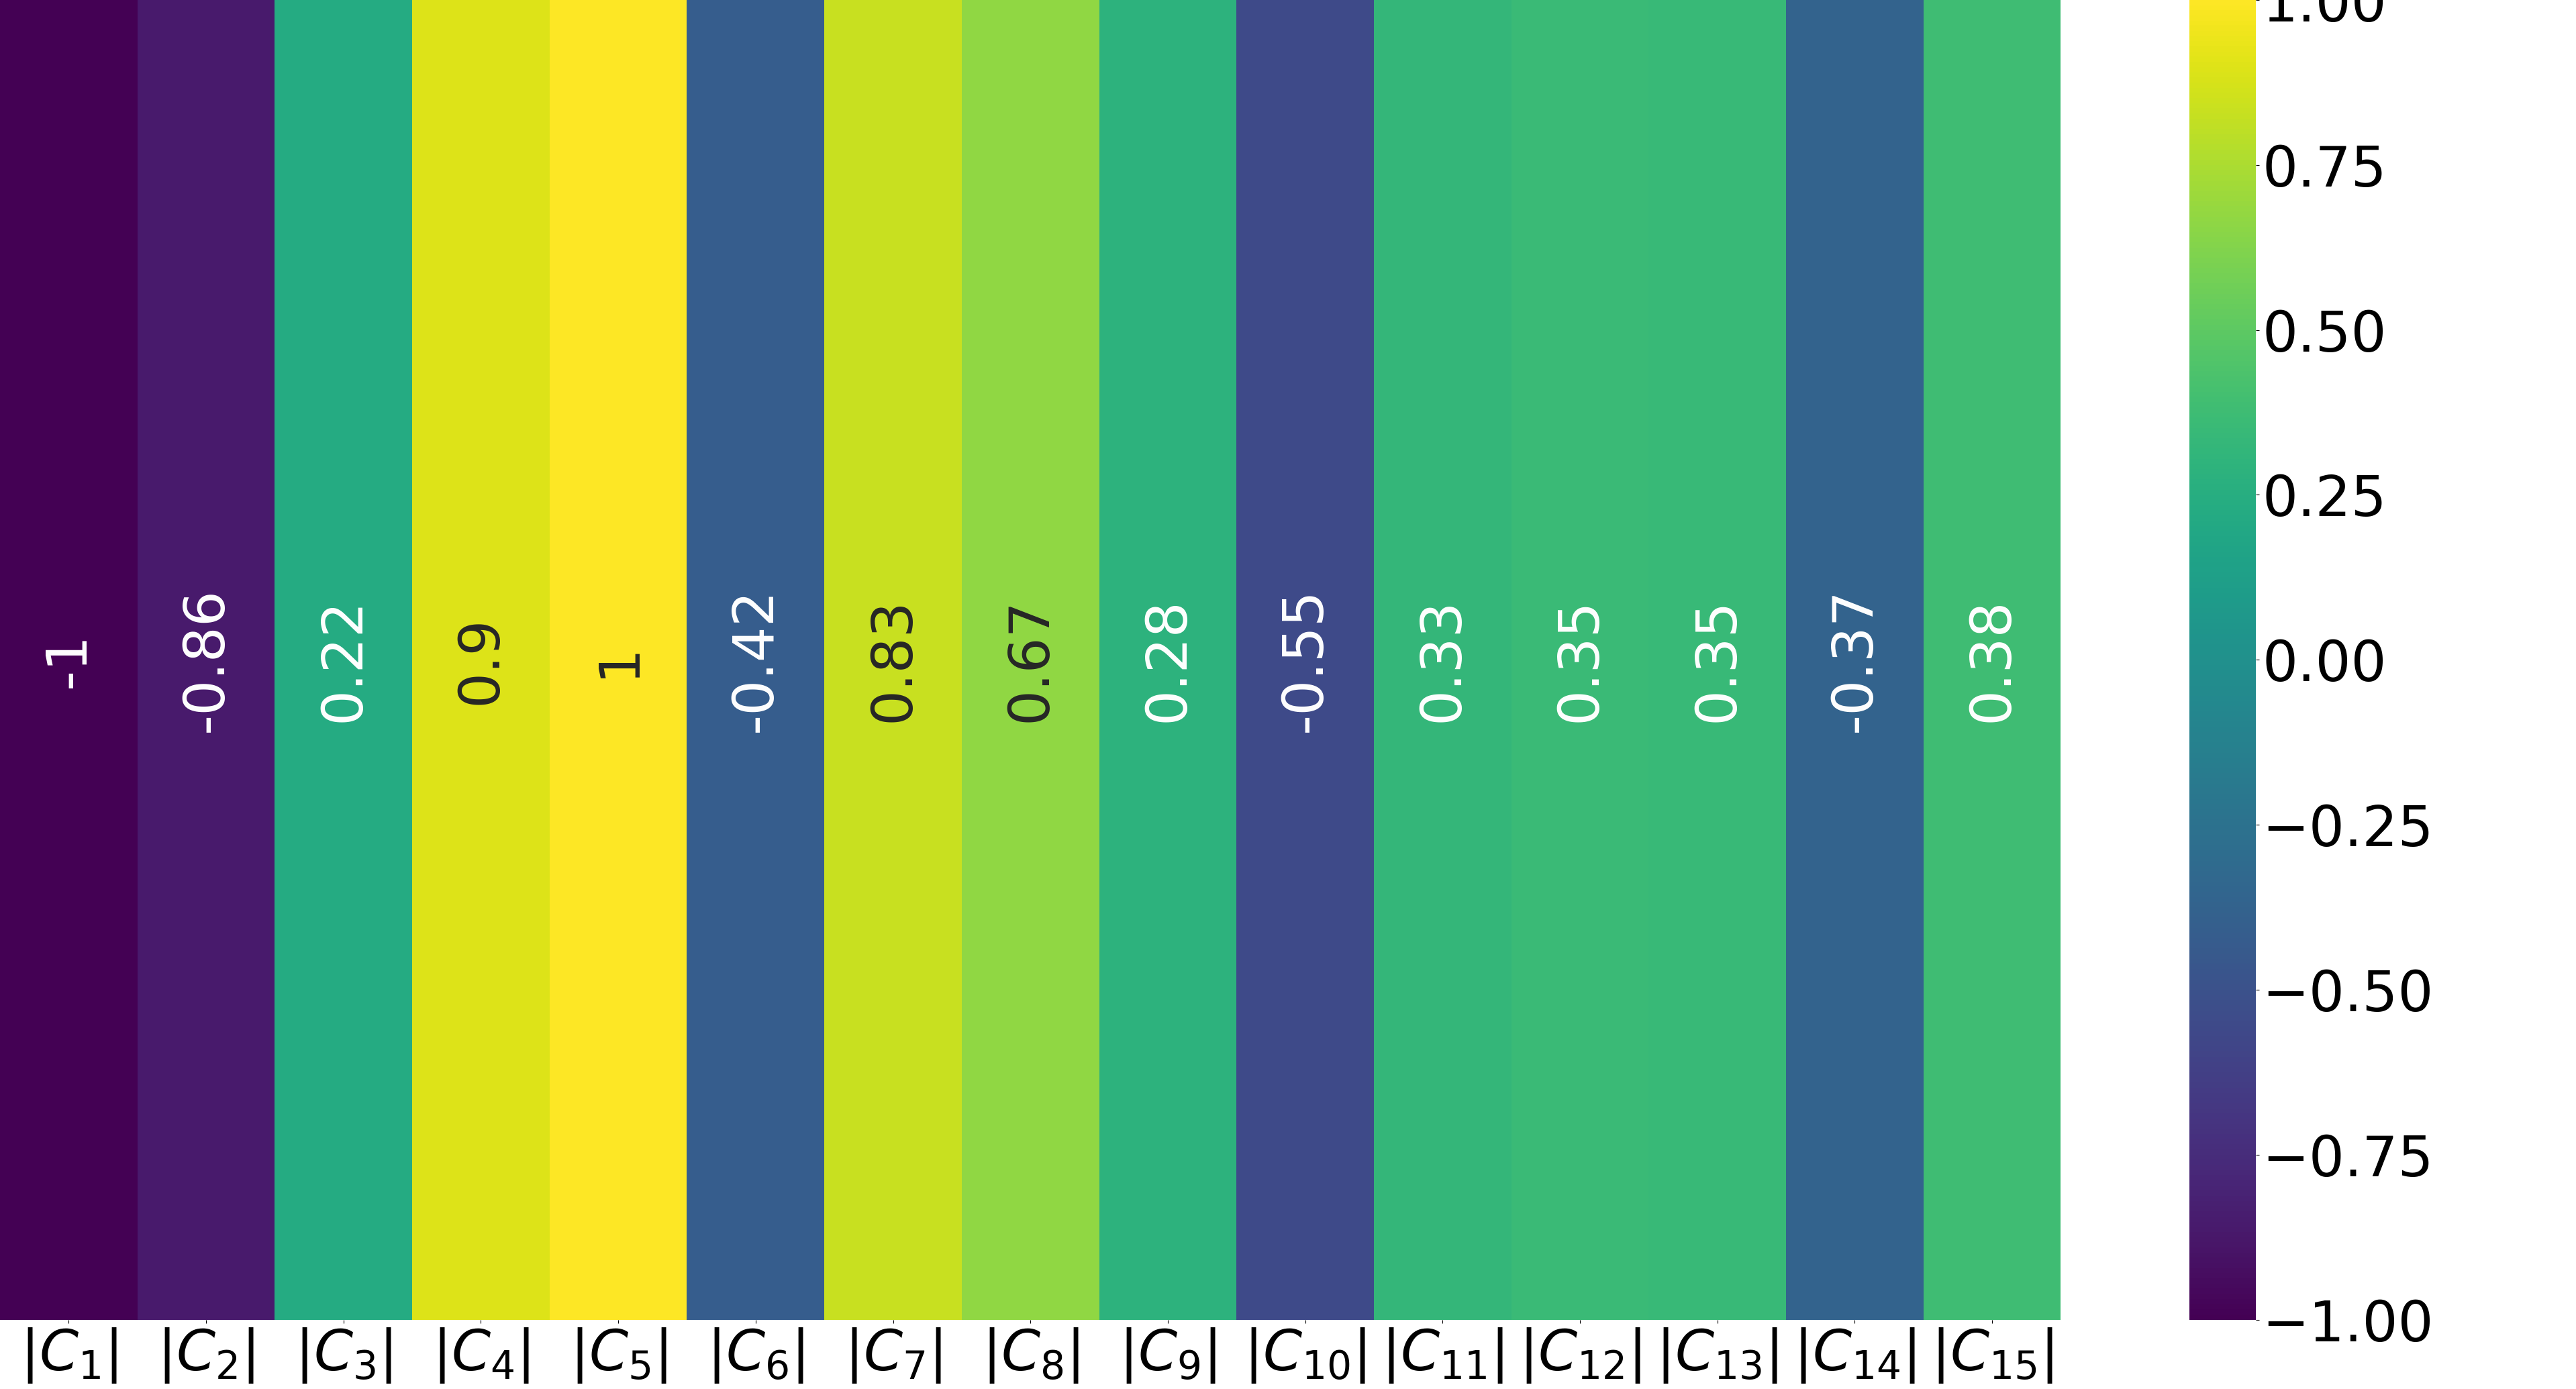
\includegraphics[width=\linewidth]{img/qlp_corr/Cnmod_coil3.png}
		\subcaption{Correlation with coil $3$}
	\end{subfigure}
	\caption{Correlation between the harmonics of the \cnmod\ attribute and the labels for \qlp.}
	\label{fig:cnmod-lcorr-qlp}
\end{figure}

\begin{figure}[!h]
	% Font size = 70
	\centering
	\begin{subfigure}{\linewidth}
		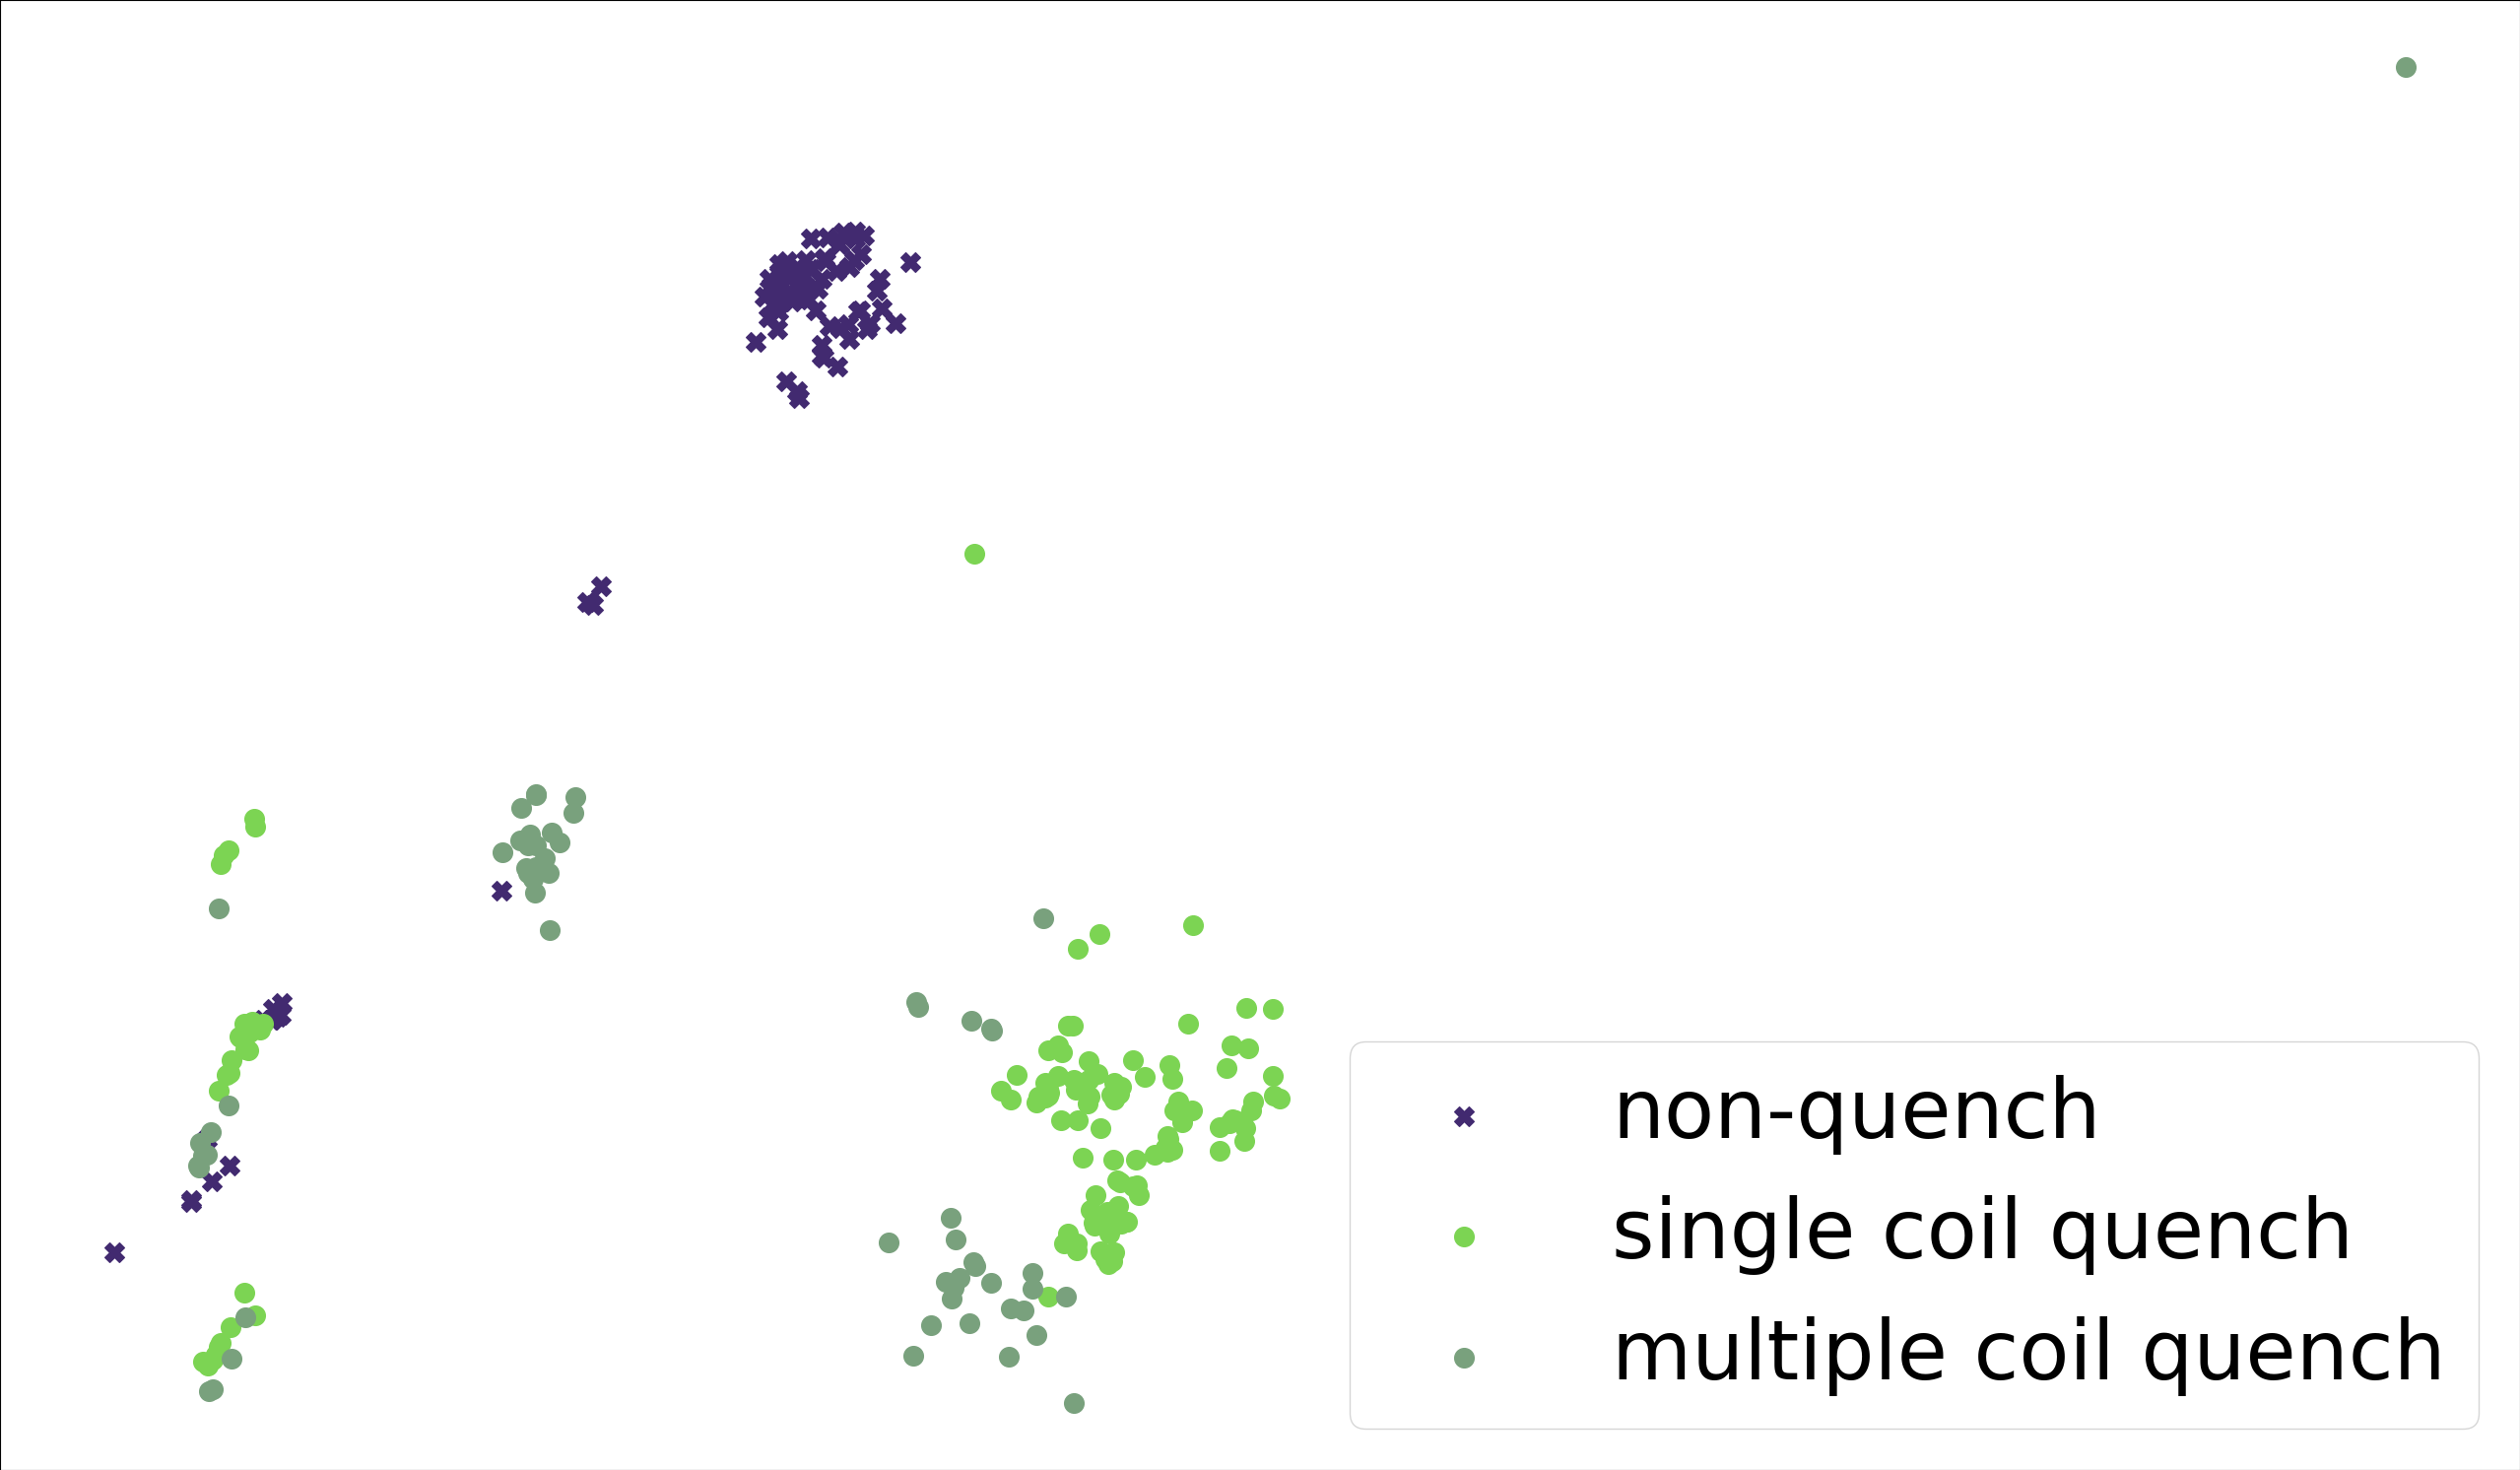
\includegraphics[width=\linewidth]{img/quench_dist_qlp/single_vs_multiple_Cnmod.png}
		\subcaption{}
	\end{subfigure}
	\begin{subfigure}{0.49\linewidth}
		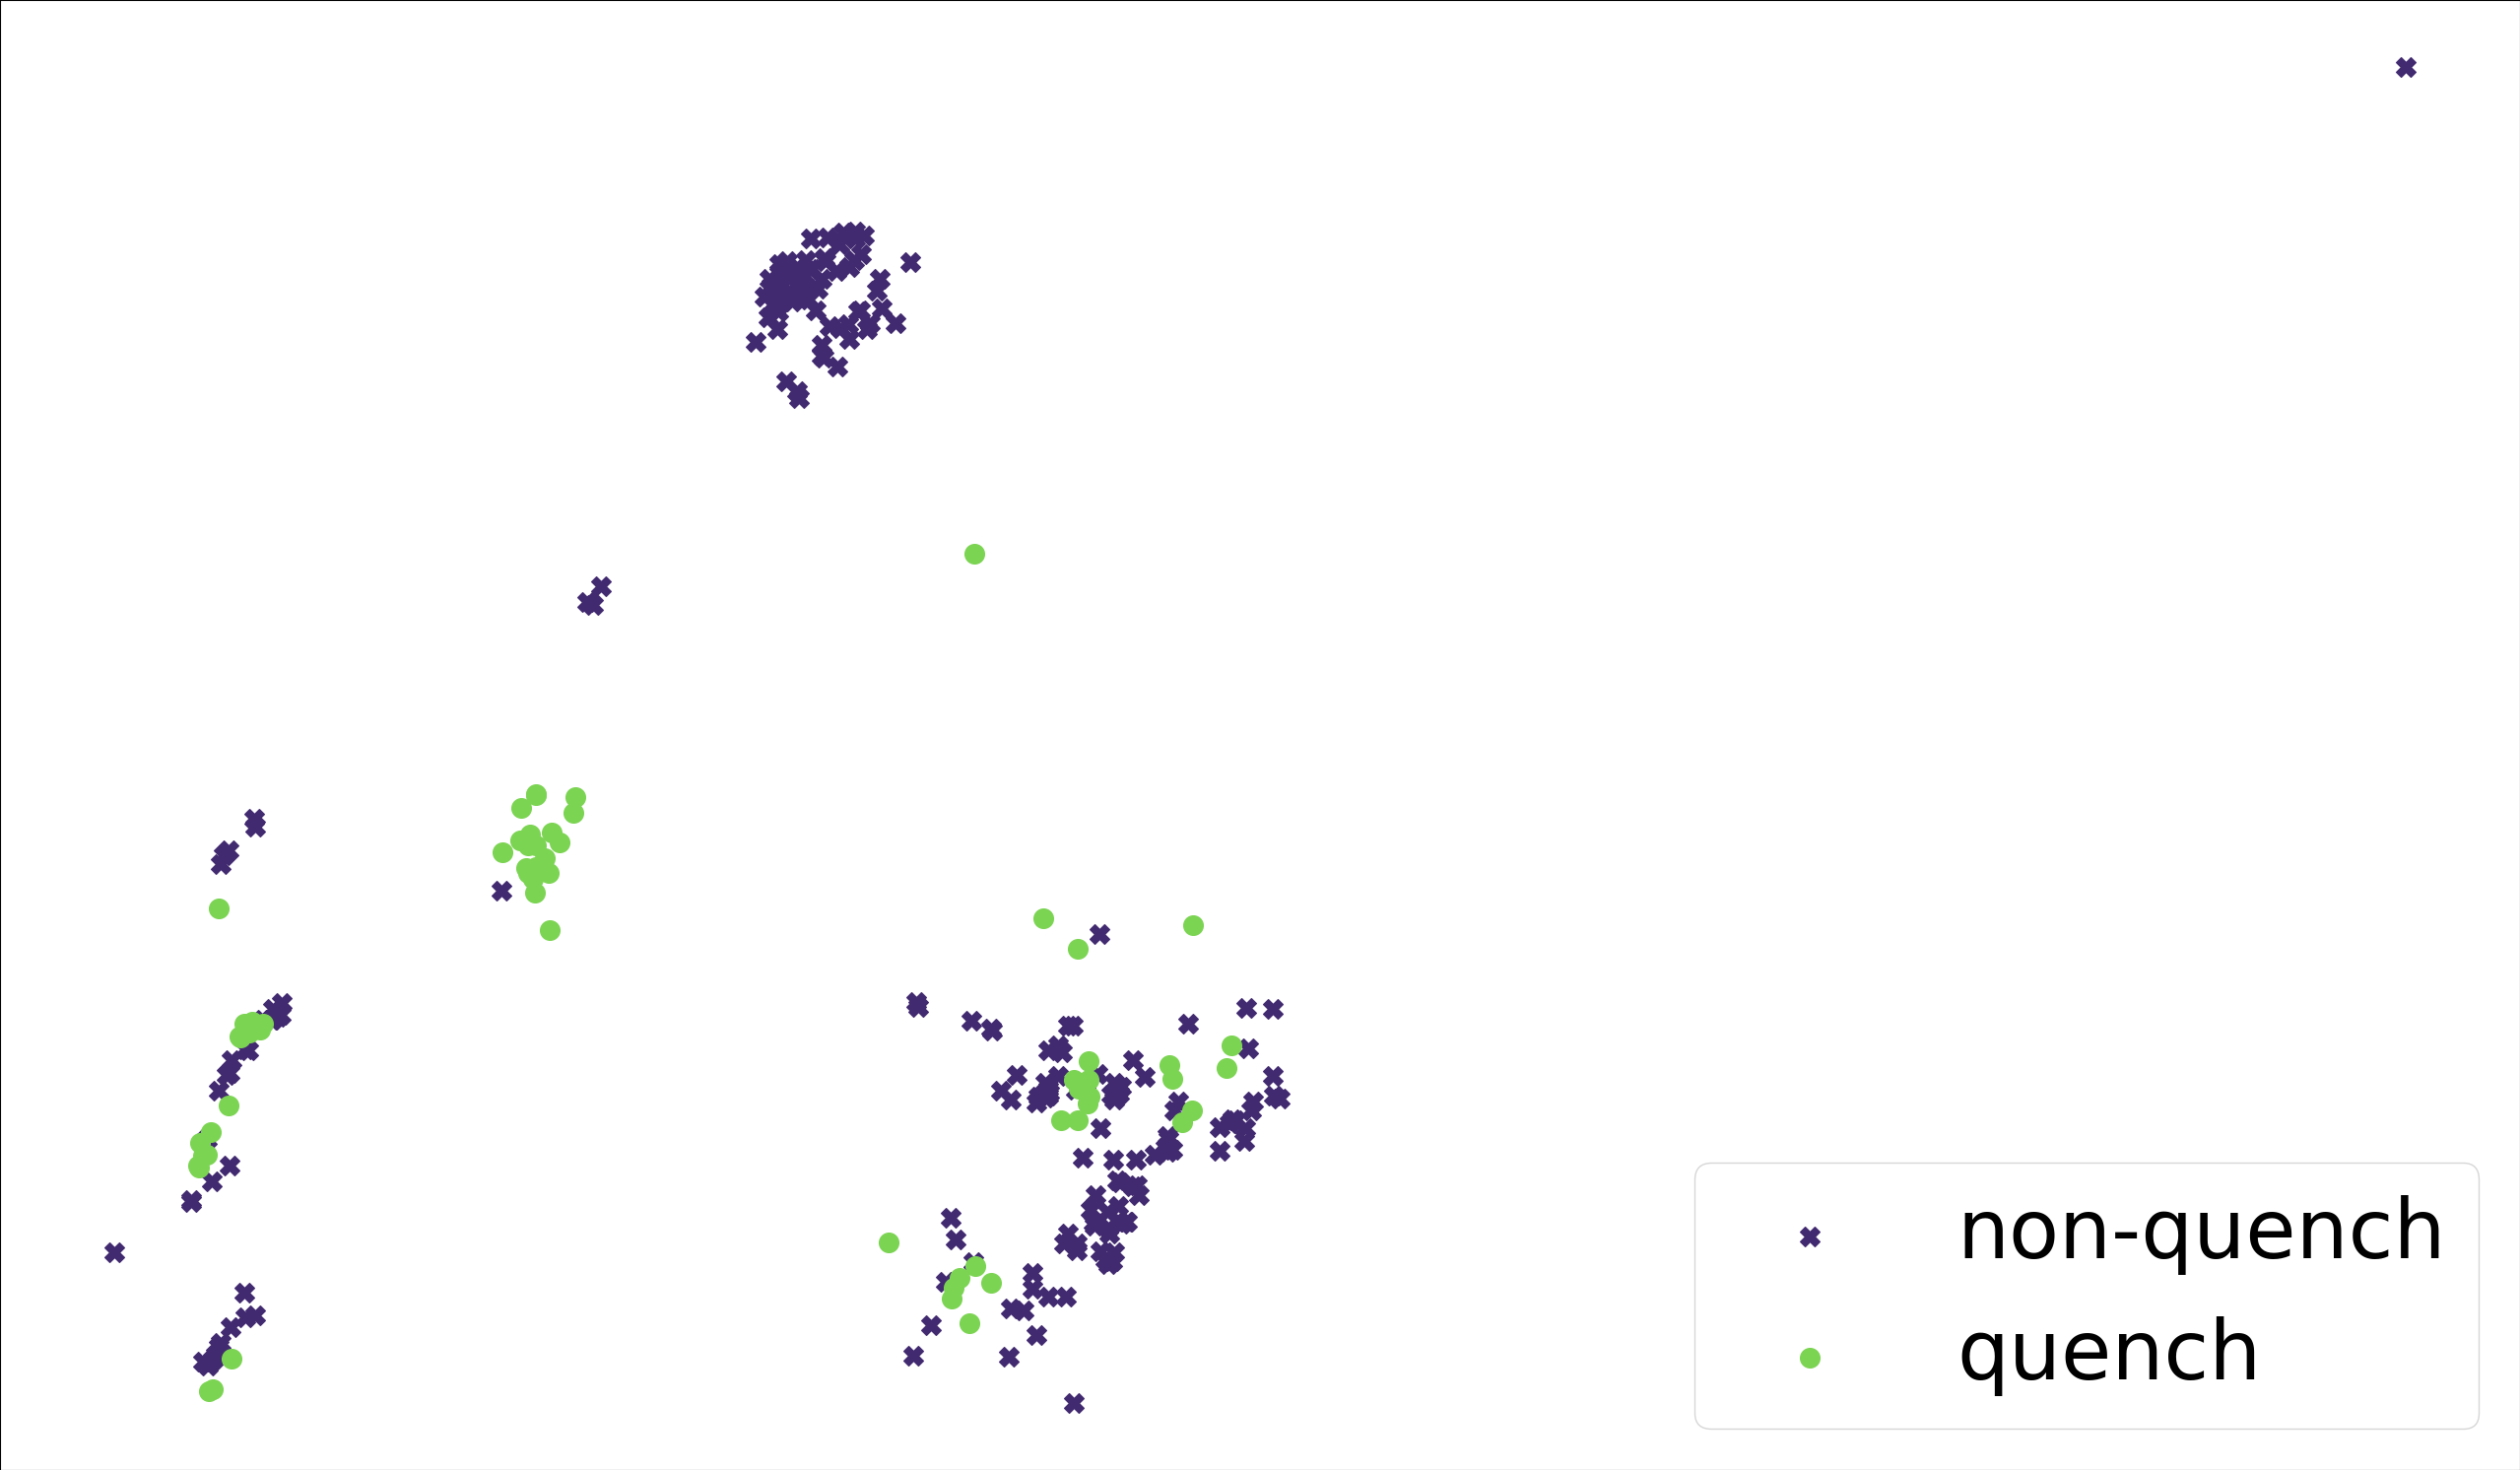
\includegraphics[width=\linewidth]{img/quench_dist_qlp/quenches_coil_0_Cnmod.png}
		\subcaption{}
	\end{subfigure}
	\begin{subfigure}{0.49\linewidth}
		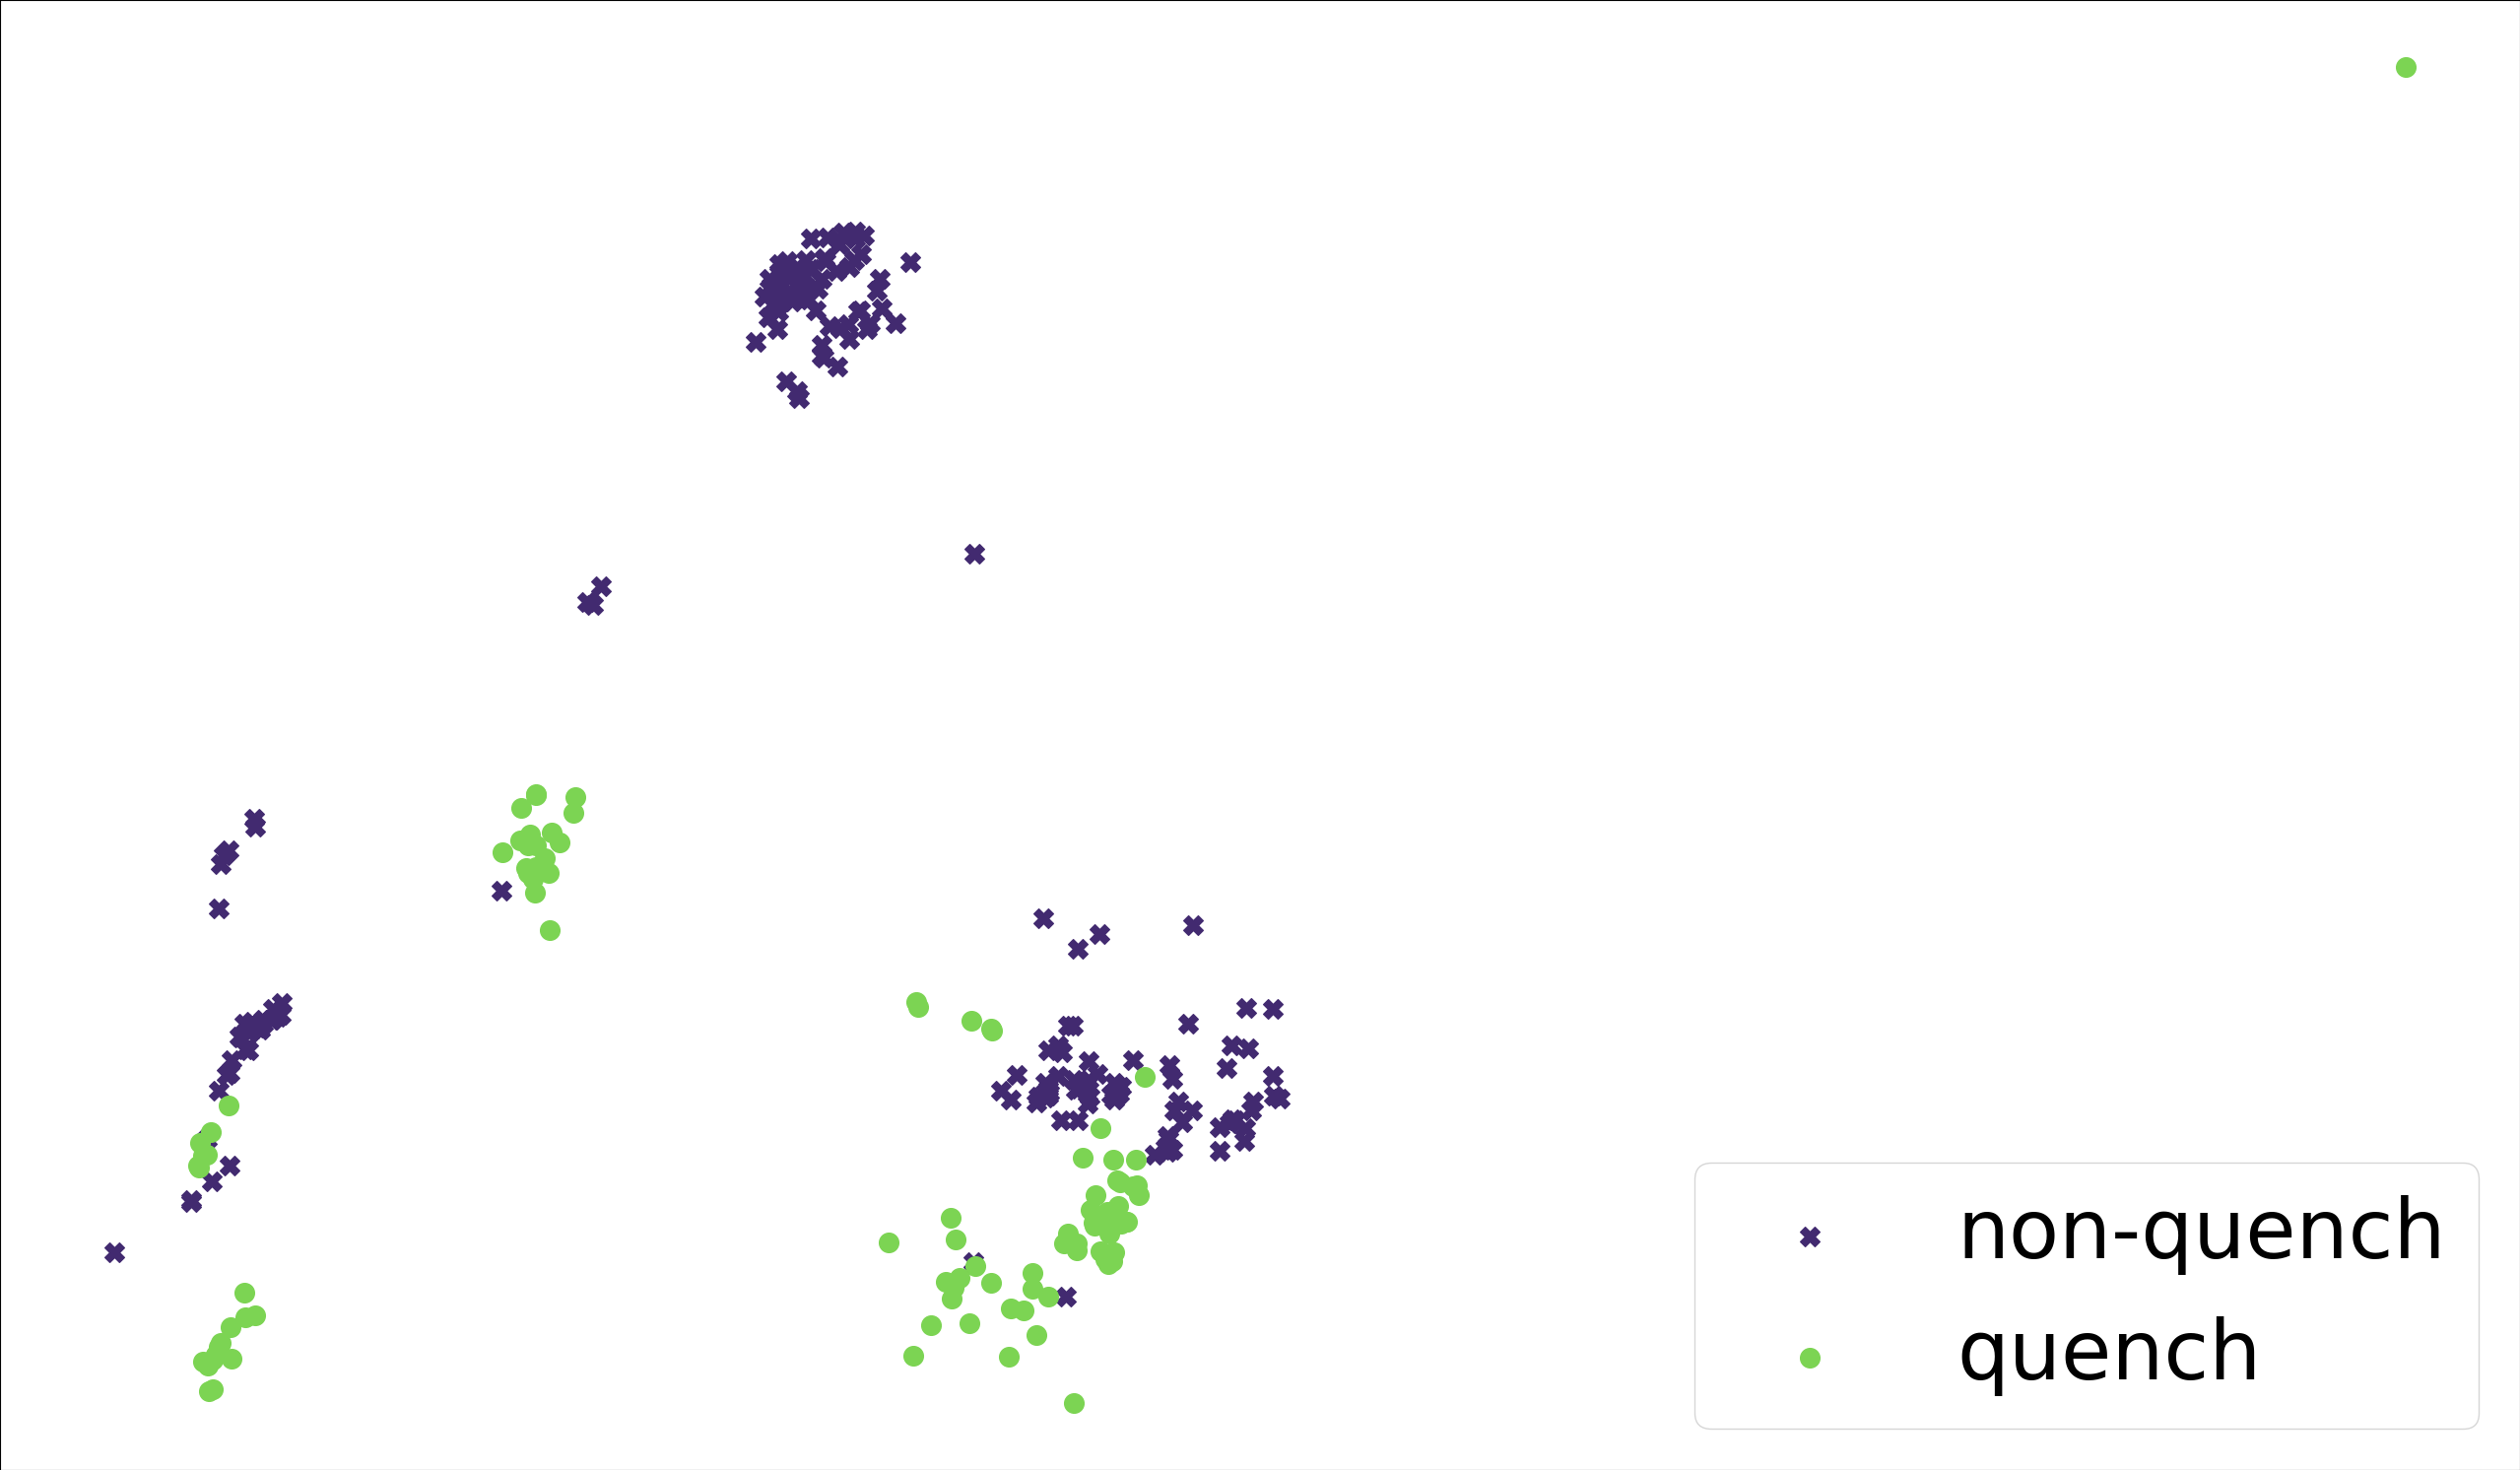
\includegraphics[width=\linewidth]{img/quench_dist_qlp/quenches_coil_1_Cnmod.png}
		\subcaption{}
	\end{subfigure}
	\begin{subfigure}{0.49\linewidth}
		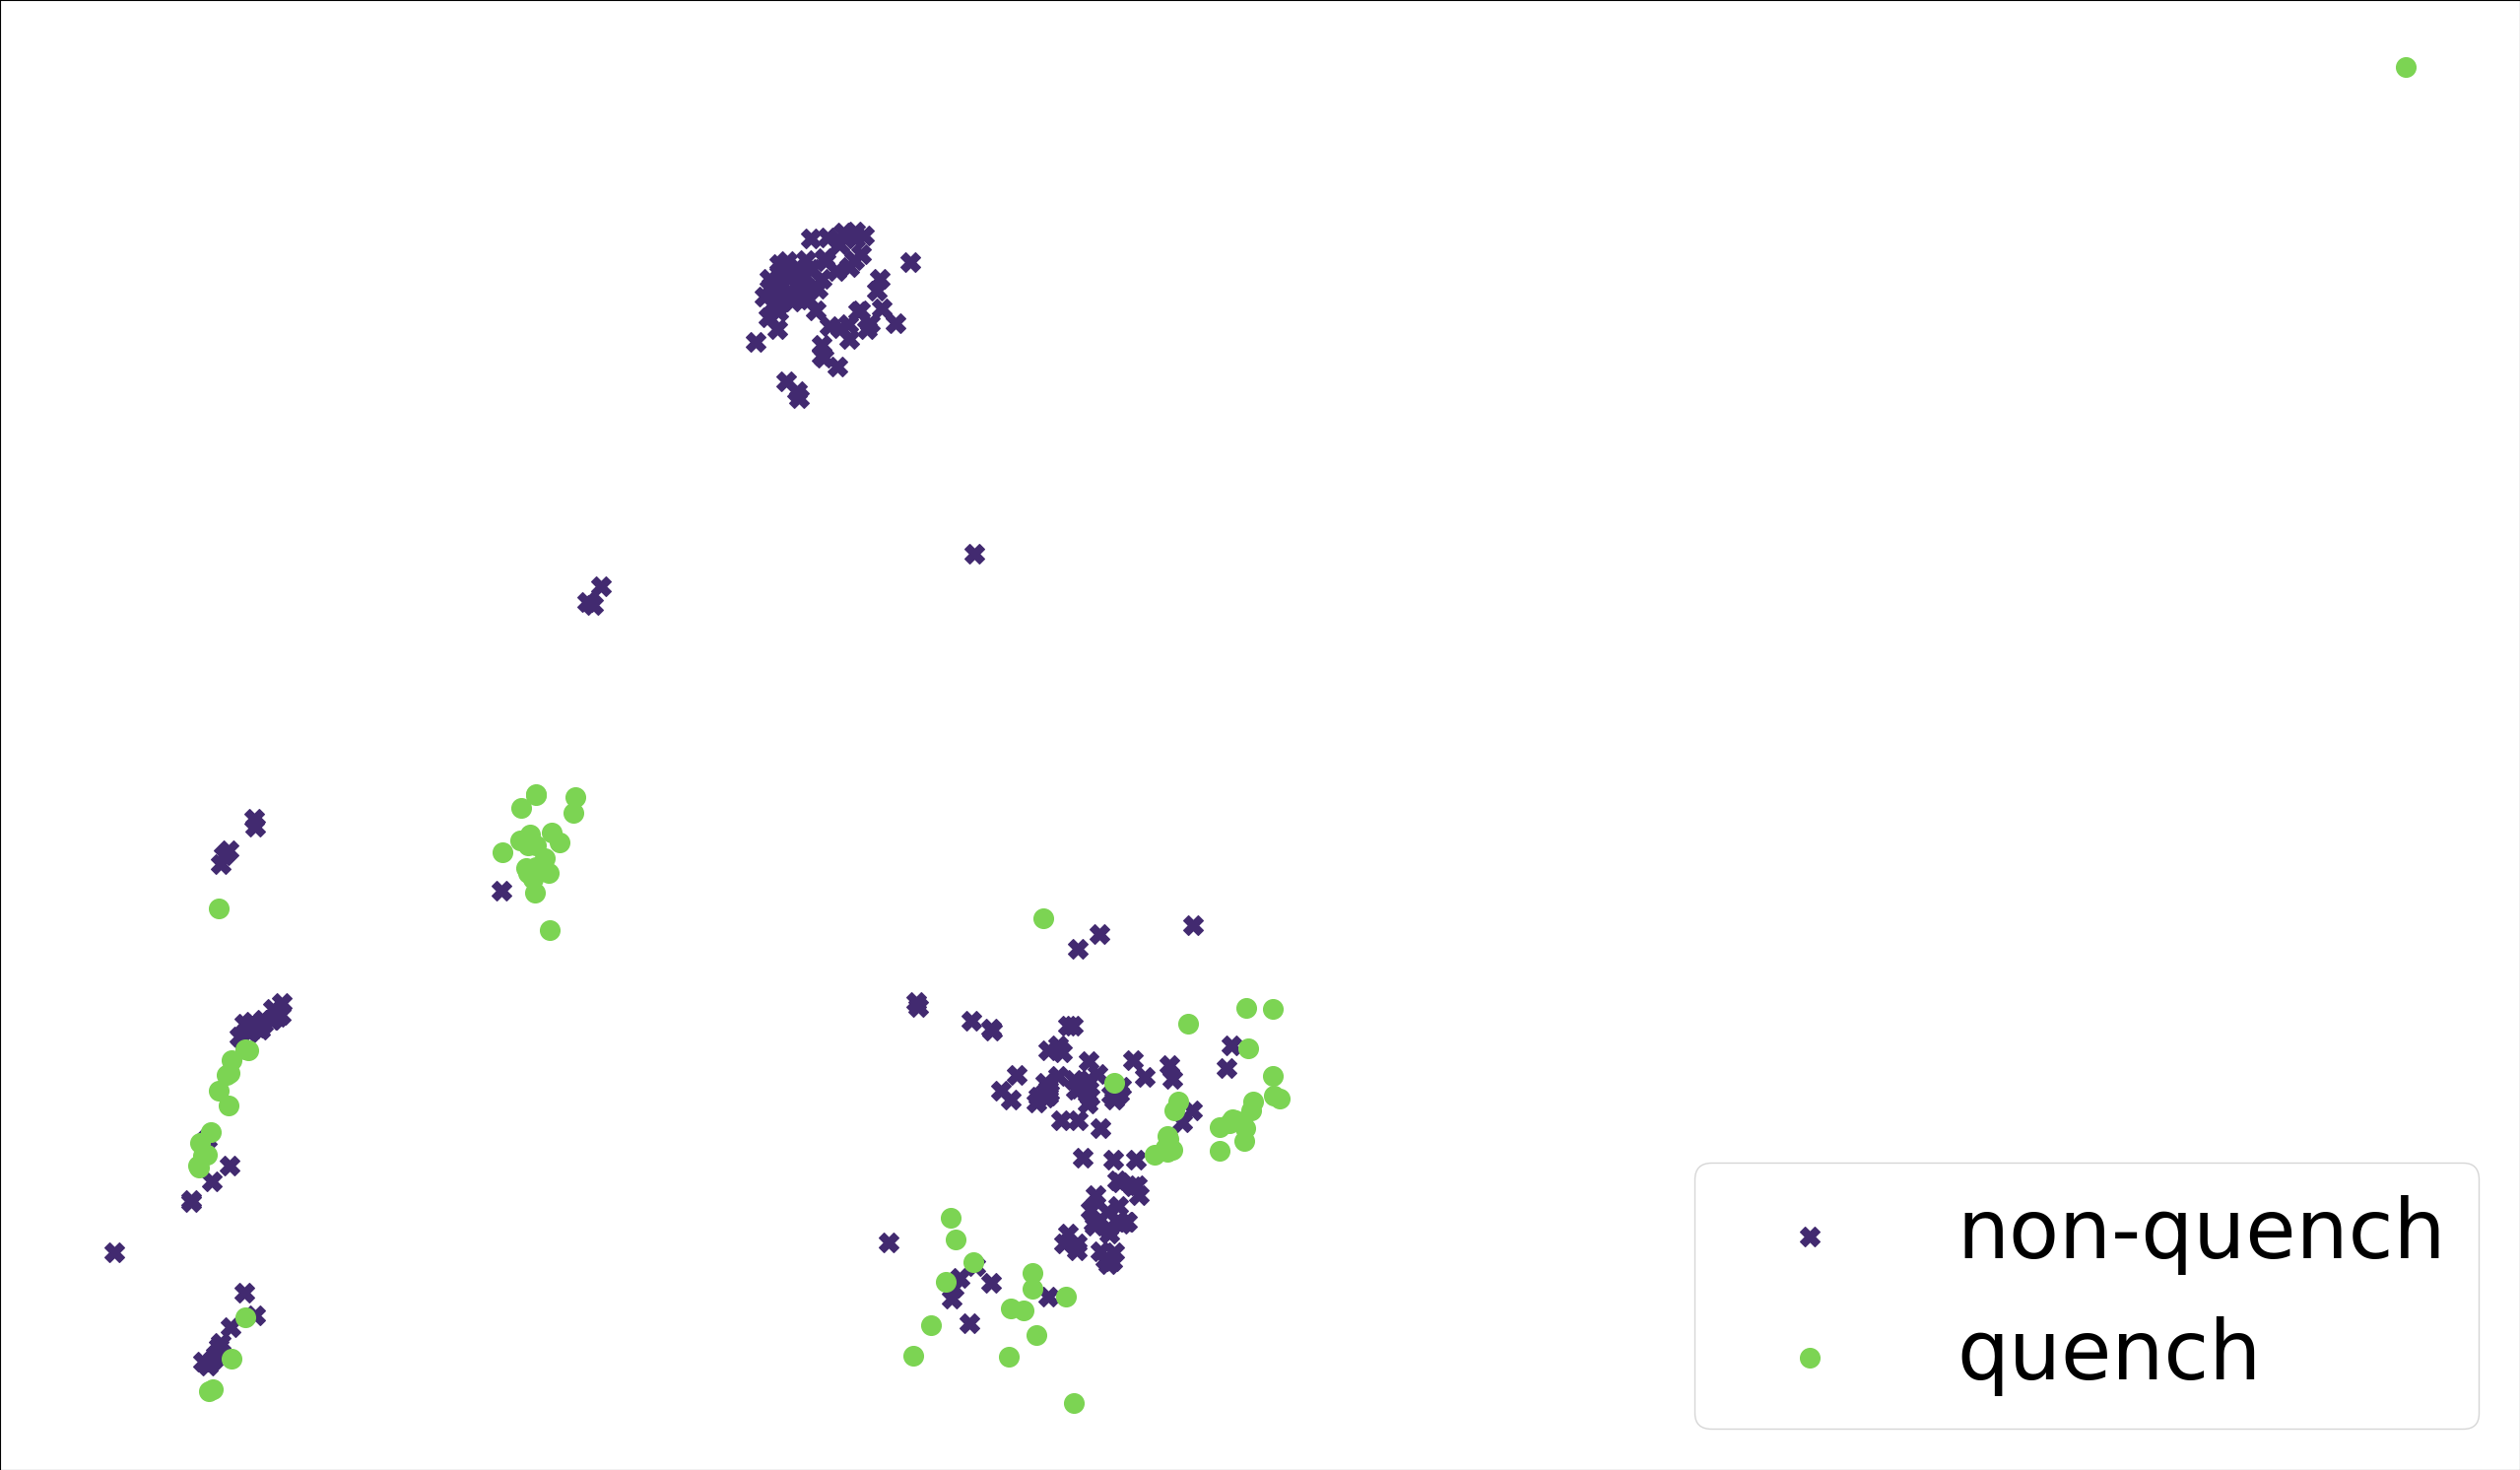
\includegraphics[width=\linewidth]{img/quench_dist_qlp/quenches_coil_2_Cnmod.png}
		\subcaption{}
	\end{subfigure}
	\begin{subfigure}{0.49\linewidth}
		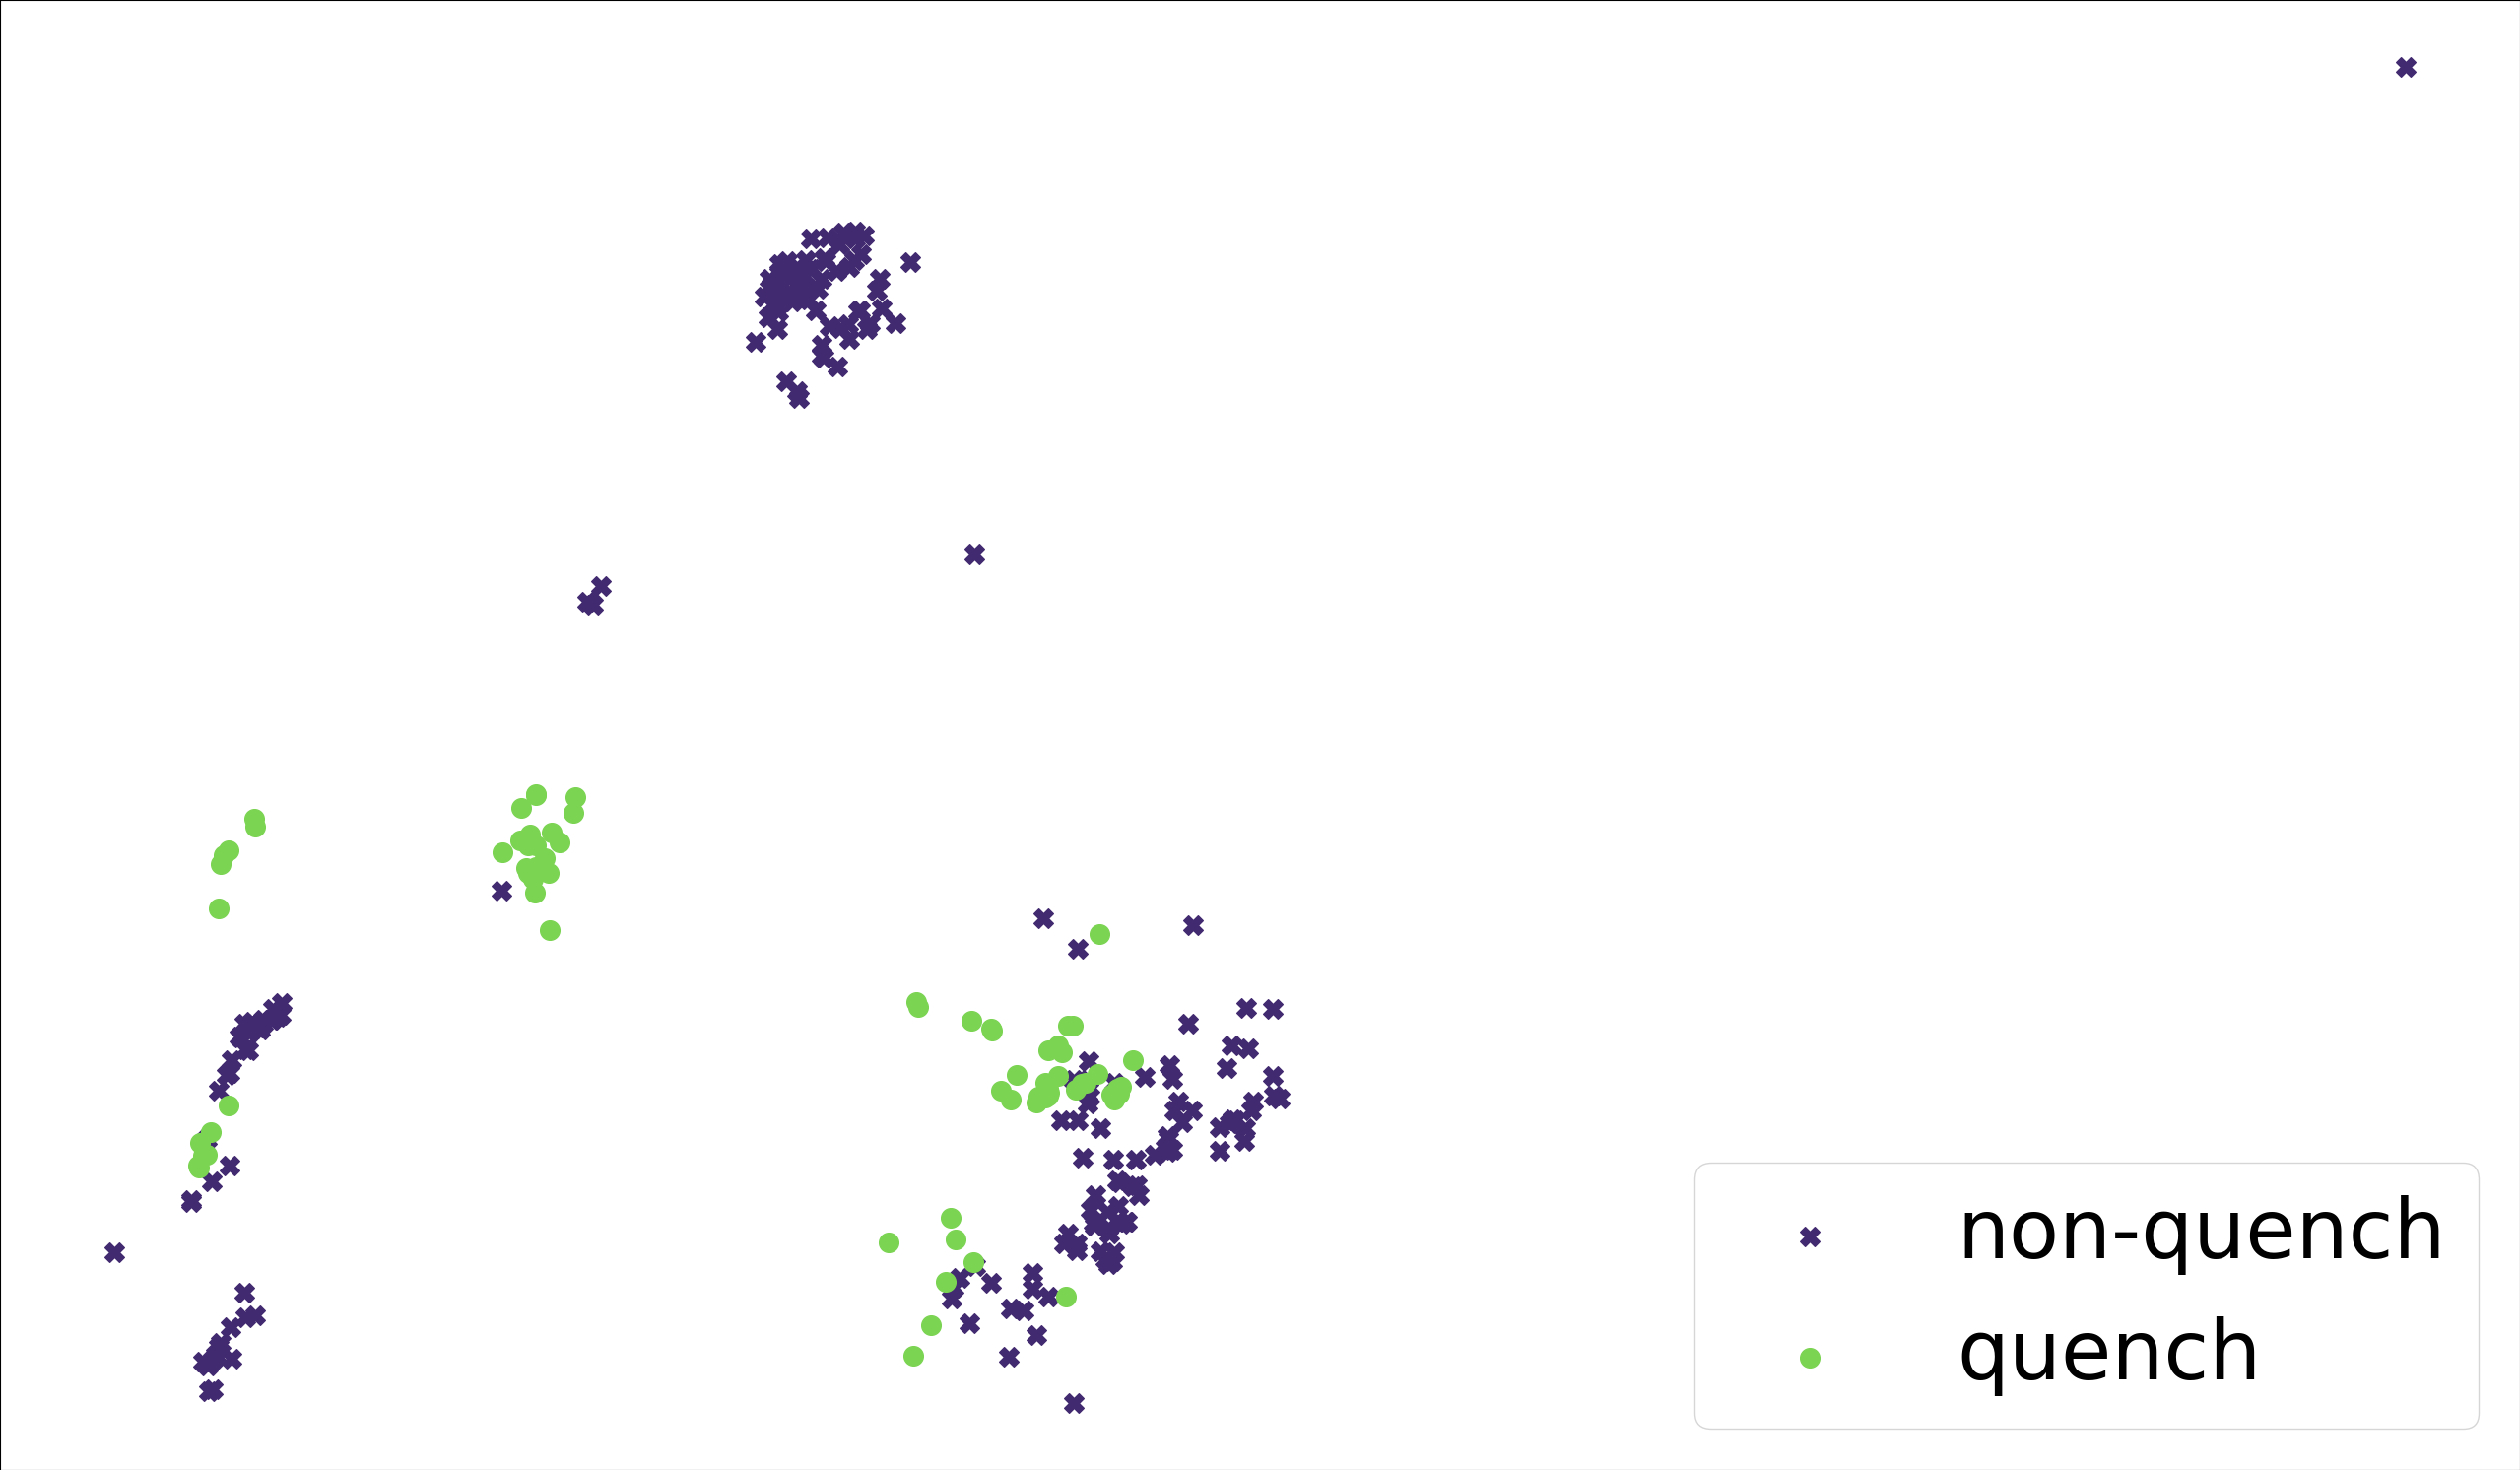
\includegraphics[width=\linewidth]{img/quench_dist_qlp/quenches_coil_3_Cnmod.png}
		\subcaption{}
	\end{subfigure}
	\caption{The distribution of the samples in bidimensional space after a round of \pca, for
		the \an\ attribute. the subfigures contain different views of the same data: (a) differenciates between non-quench and single or multiple quench events, (b) highlights the distribution of quenches for coil $0$, (c) highlights the distribution of quenches for coil $1$, (d) highlights the distribution of quenches for coil $2$ and finally (e) highlights the distribution of quenches for coil $3$.}
	\label{fig:cnmod-coilq-dist}
\end{figure}


\subsubsection{\phin}
\begin{figure}[!h]
	% Font size = 70
	\centering
	\begin{subfigure}{0.49\linewidth}
		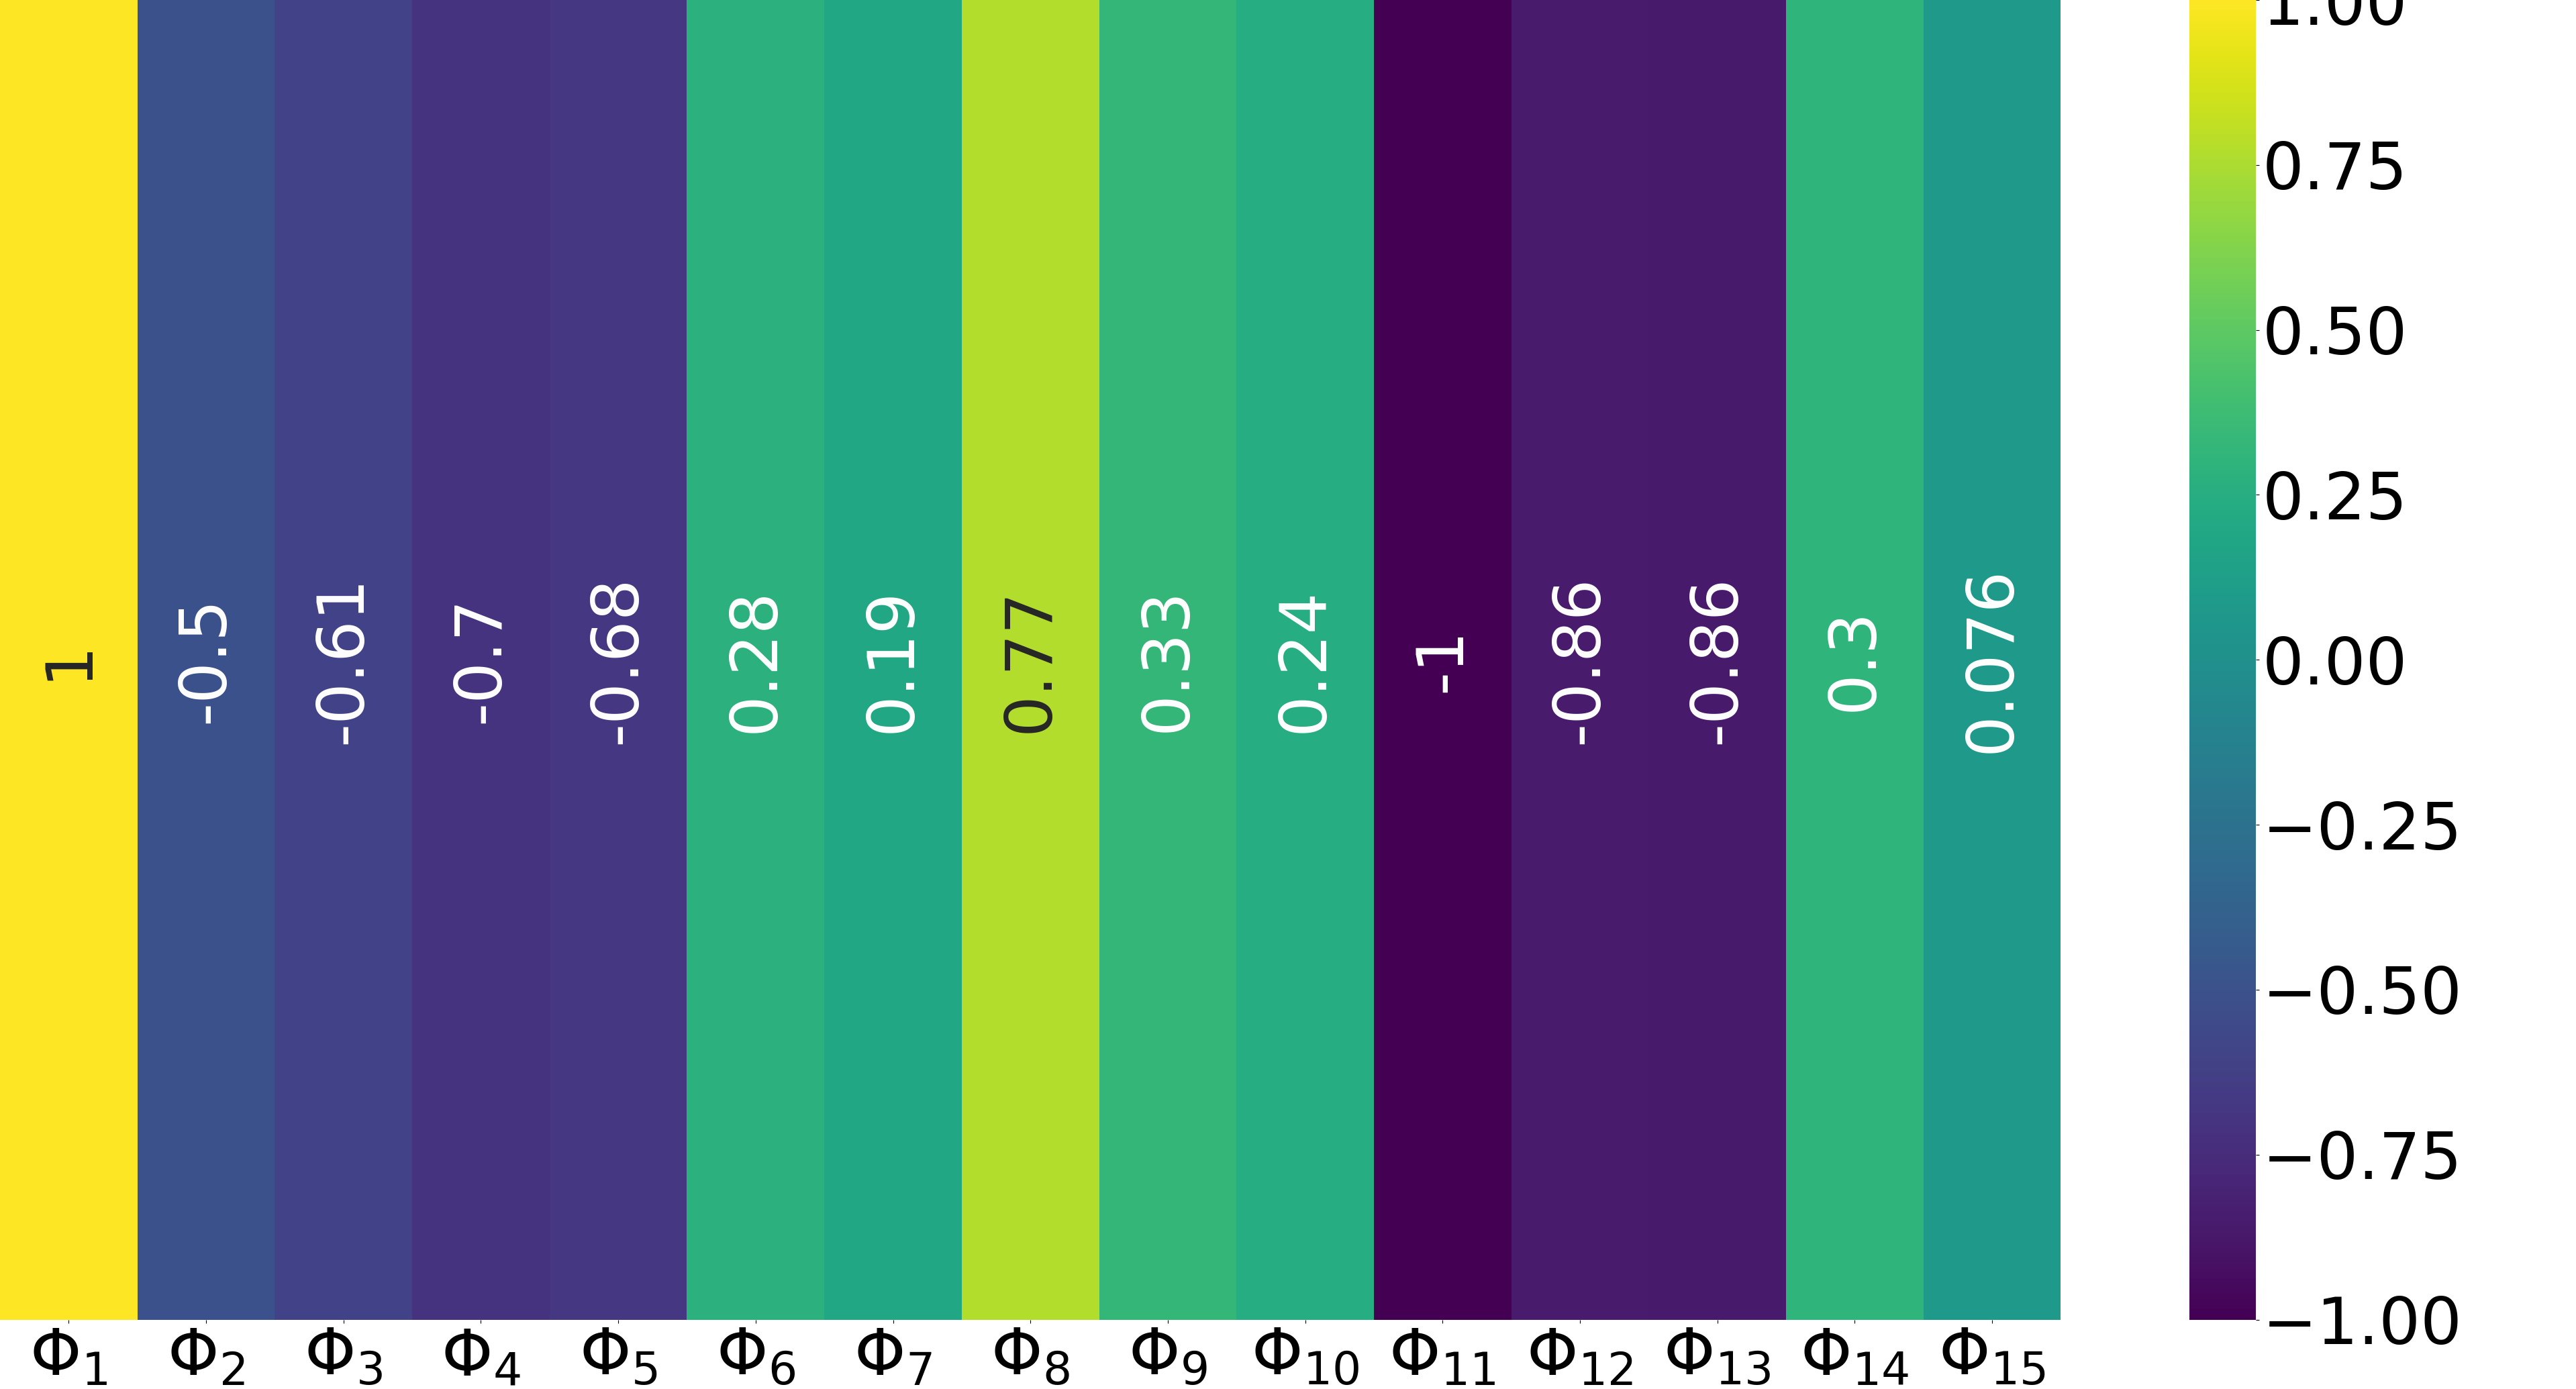
\includegraphics[width=\linewidth]{img/qlp_corr/Phi_coil0.png}
		\subcaption{Correlation with coil $0$}
	\end{subfigure}
	\begin{subfigure}{0.49\linewidth}
		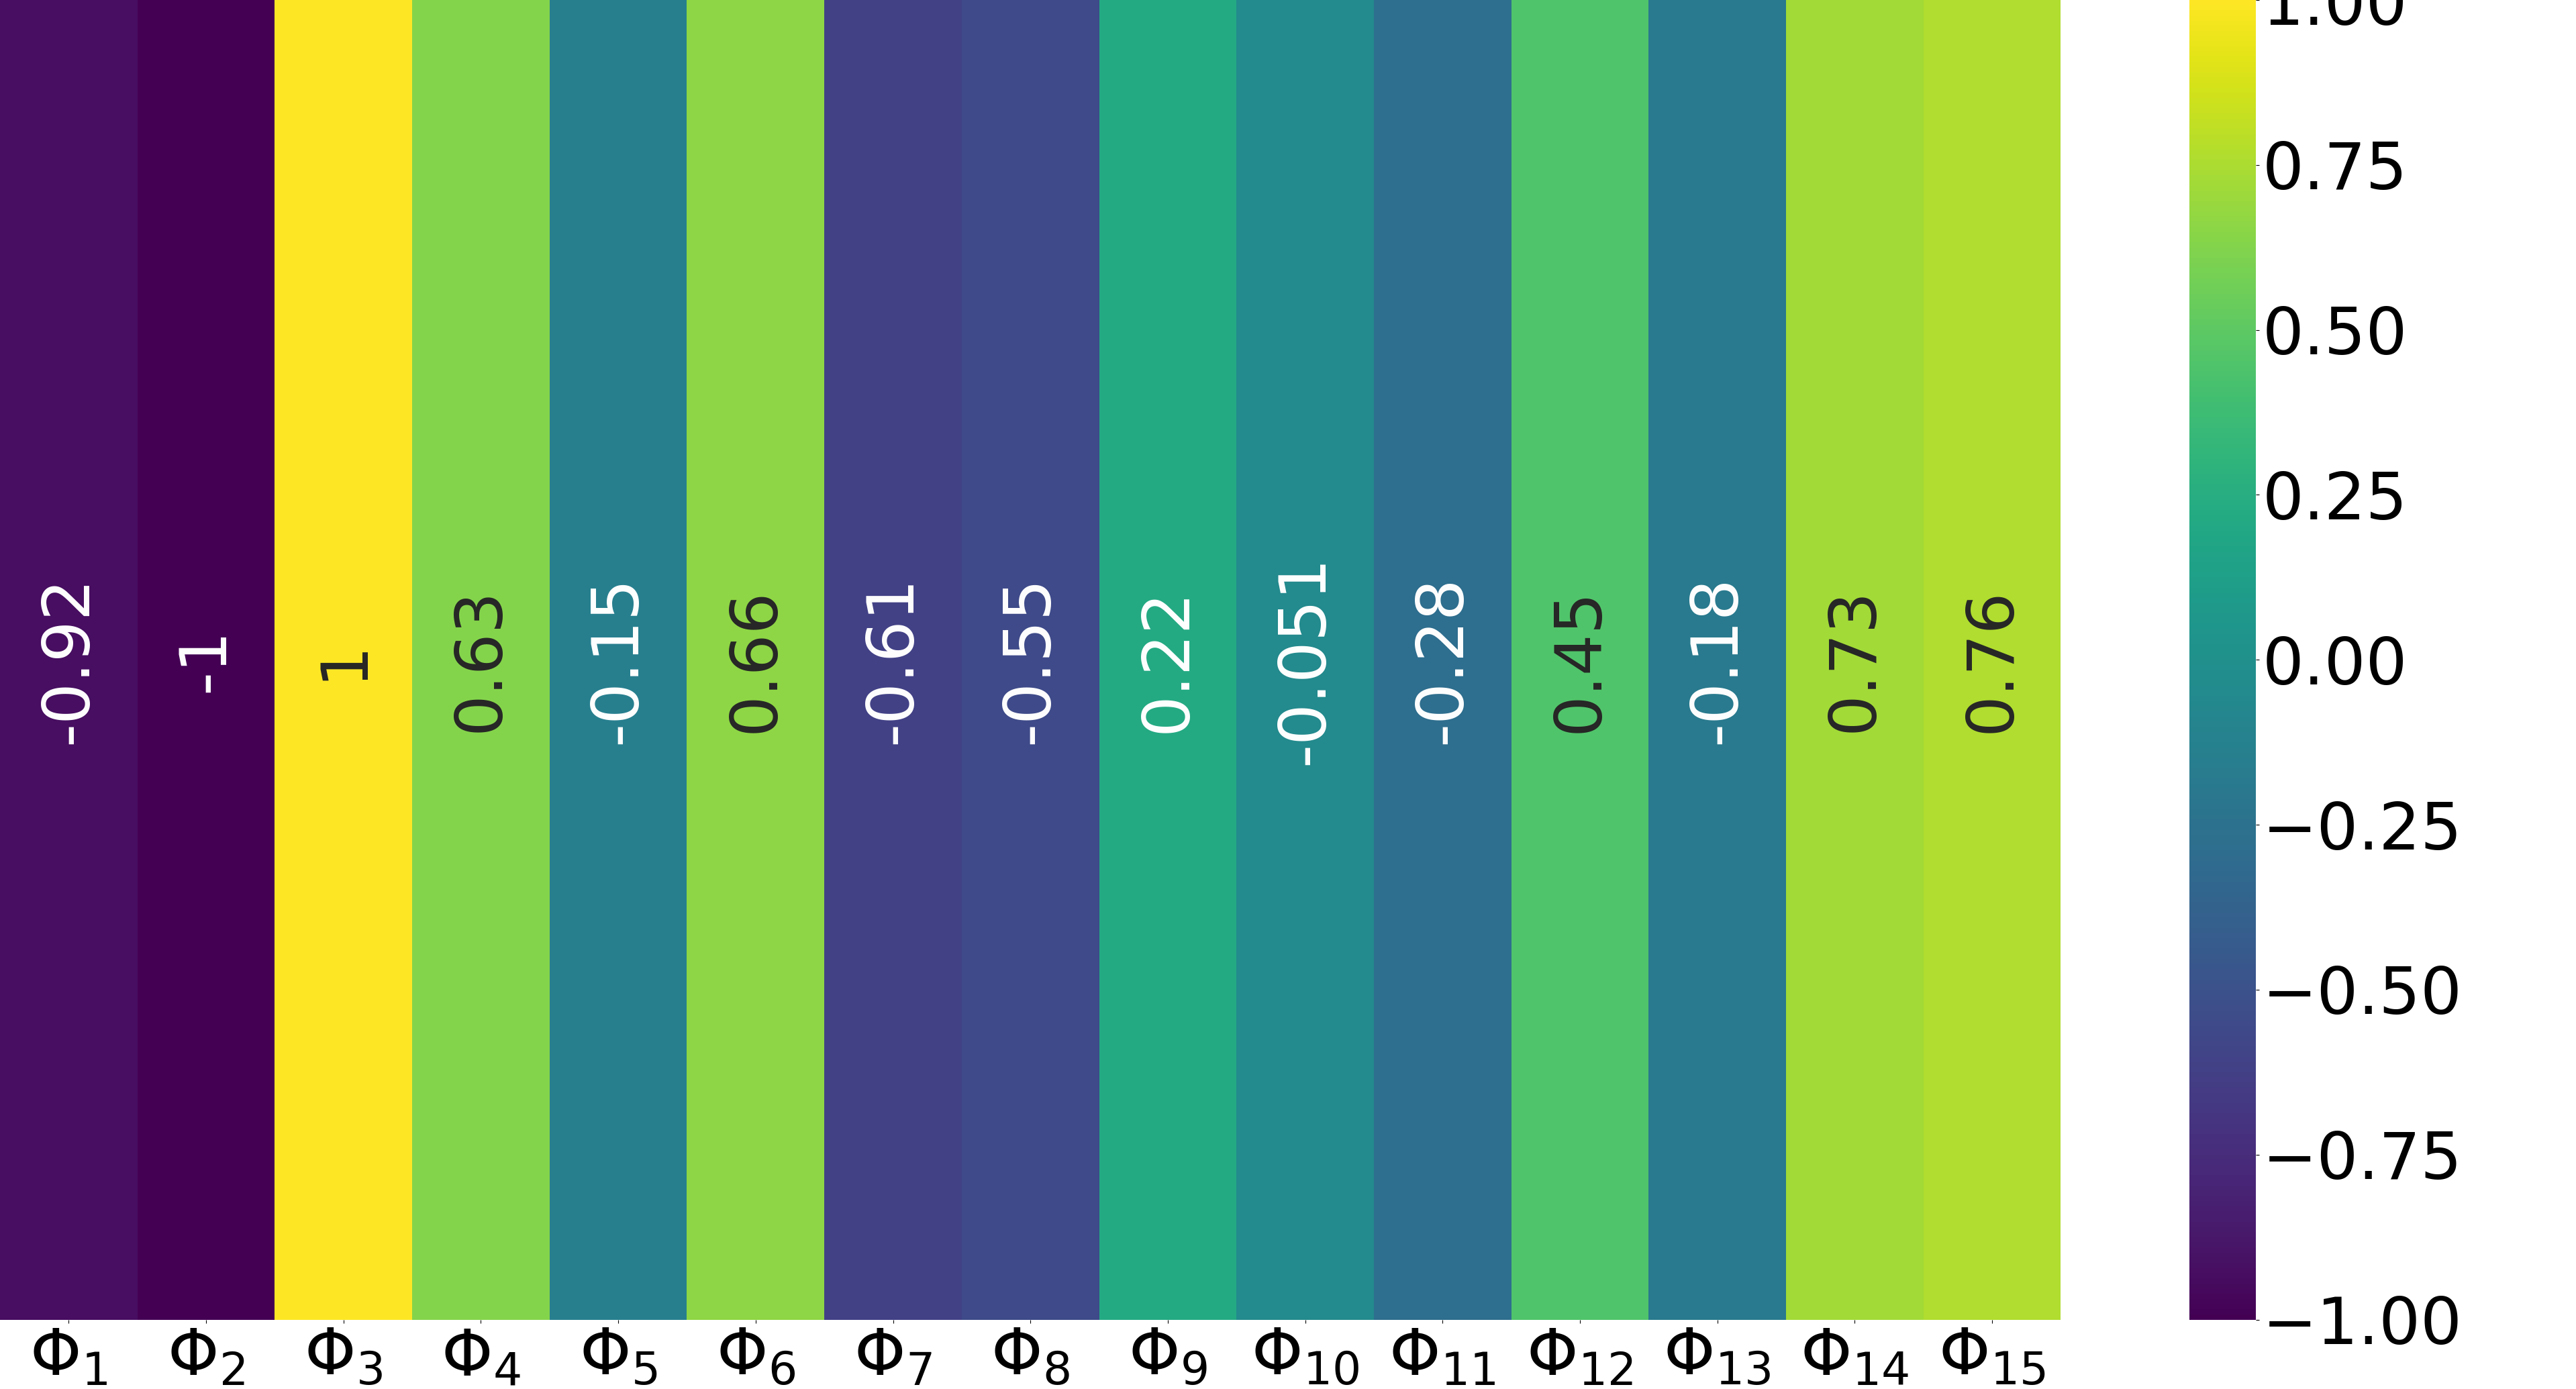
\includegraphics[width=\linewidth]{img/qlp_corr/Phi_coil1.png}
		\subcaption{Correlation with coil $1$}
	\end{subfigure}
	\begin{subfigure}{0.49\linewidth}
		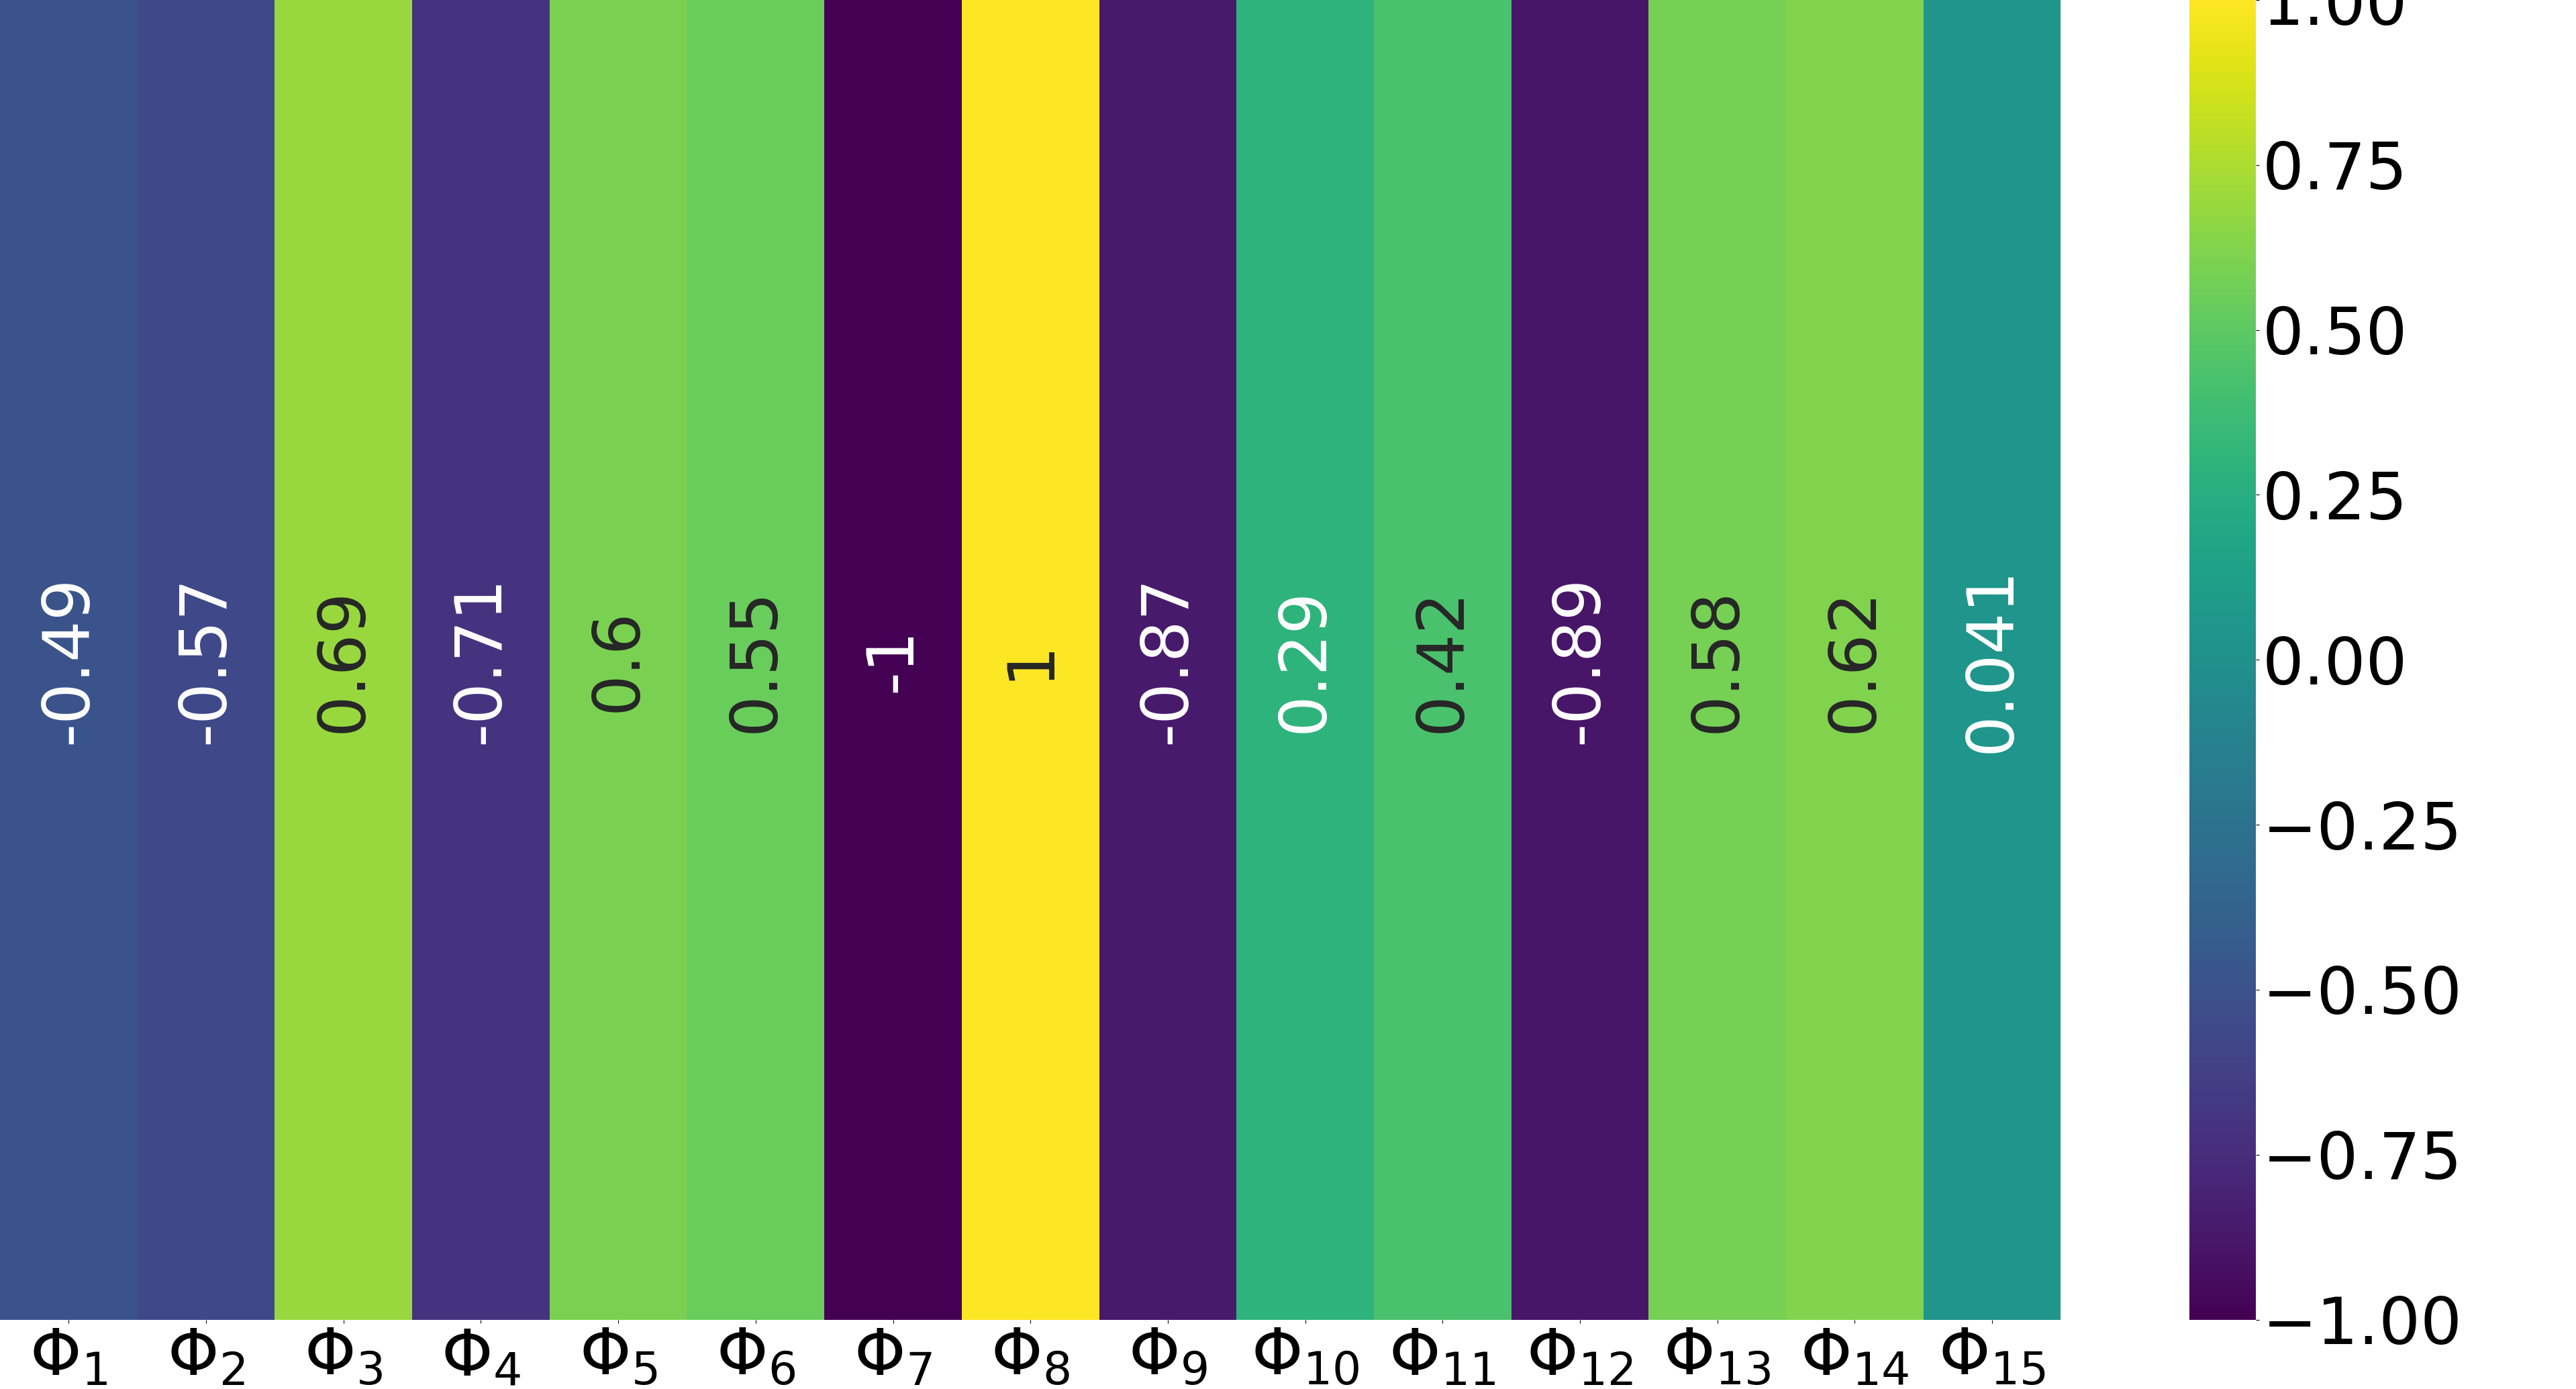
\includegraphics[width=\linewidth]{img/qlp_corr/Phi_coil2.png}
		\subcaption{Correlation with coil $2$}
	\end{subfigure}
	\begin{subfigure}{0.49\linewidth}
		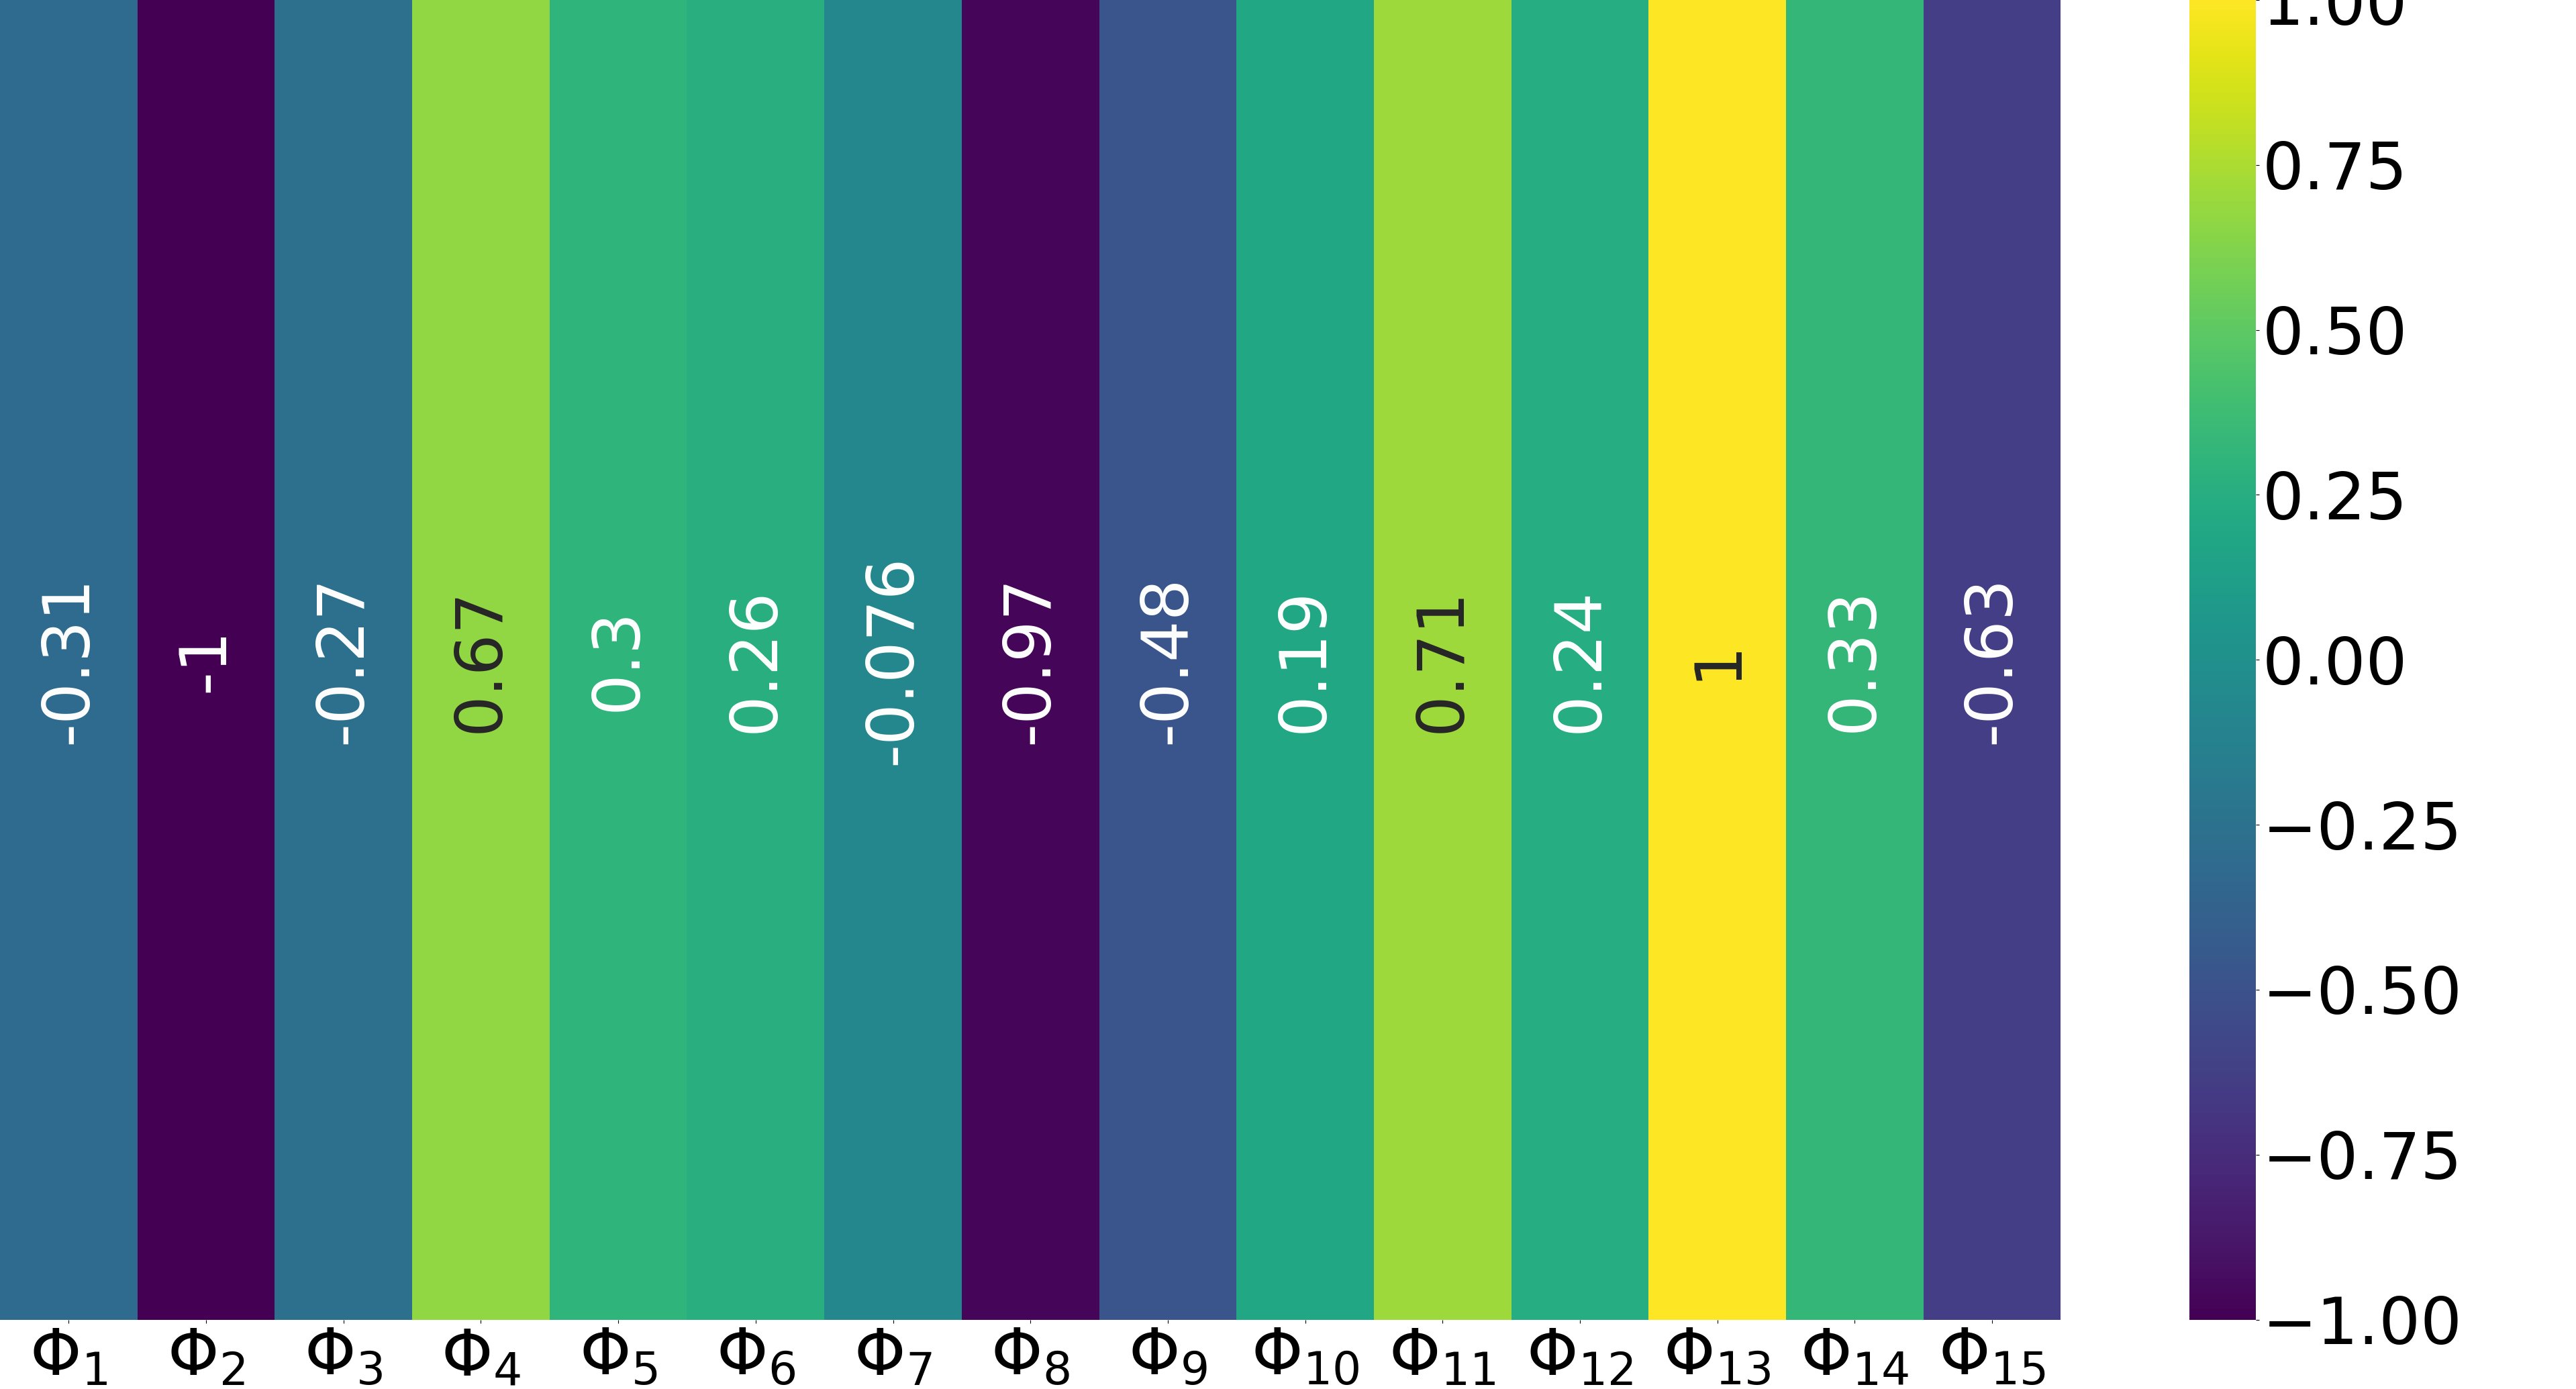
\includegraphics[width=\linewidth]{img/qlp_corr/Phi_coil3.png}
		\subcaption{Correlation with coil $3$}
	\end{subfigure}
	\caption{Correlation between the harmonics of the \cnmod\ attribute and the labels for \qlp.}
	\label{fig:phi-lcorr-qlp}
\end{figure}

\begin{figure}[!h]
	% Font size = 70
	\centering
	\begin{subfigure}{\linewidth}
		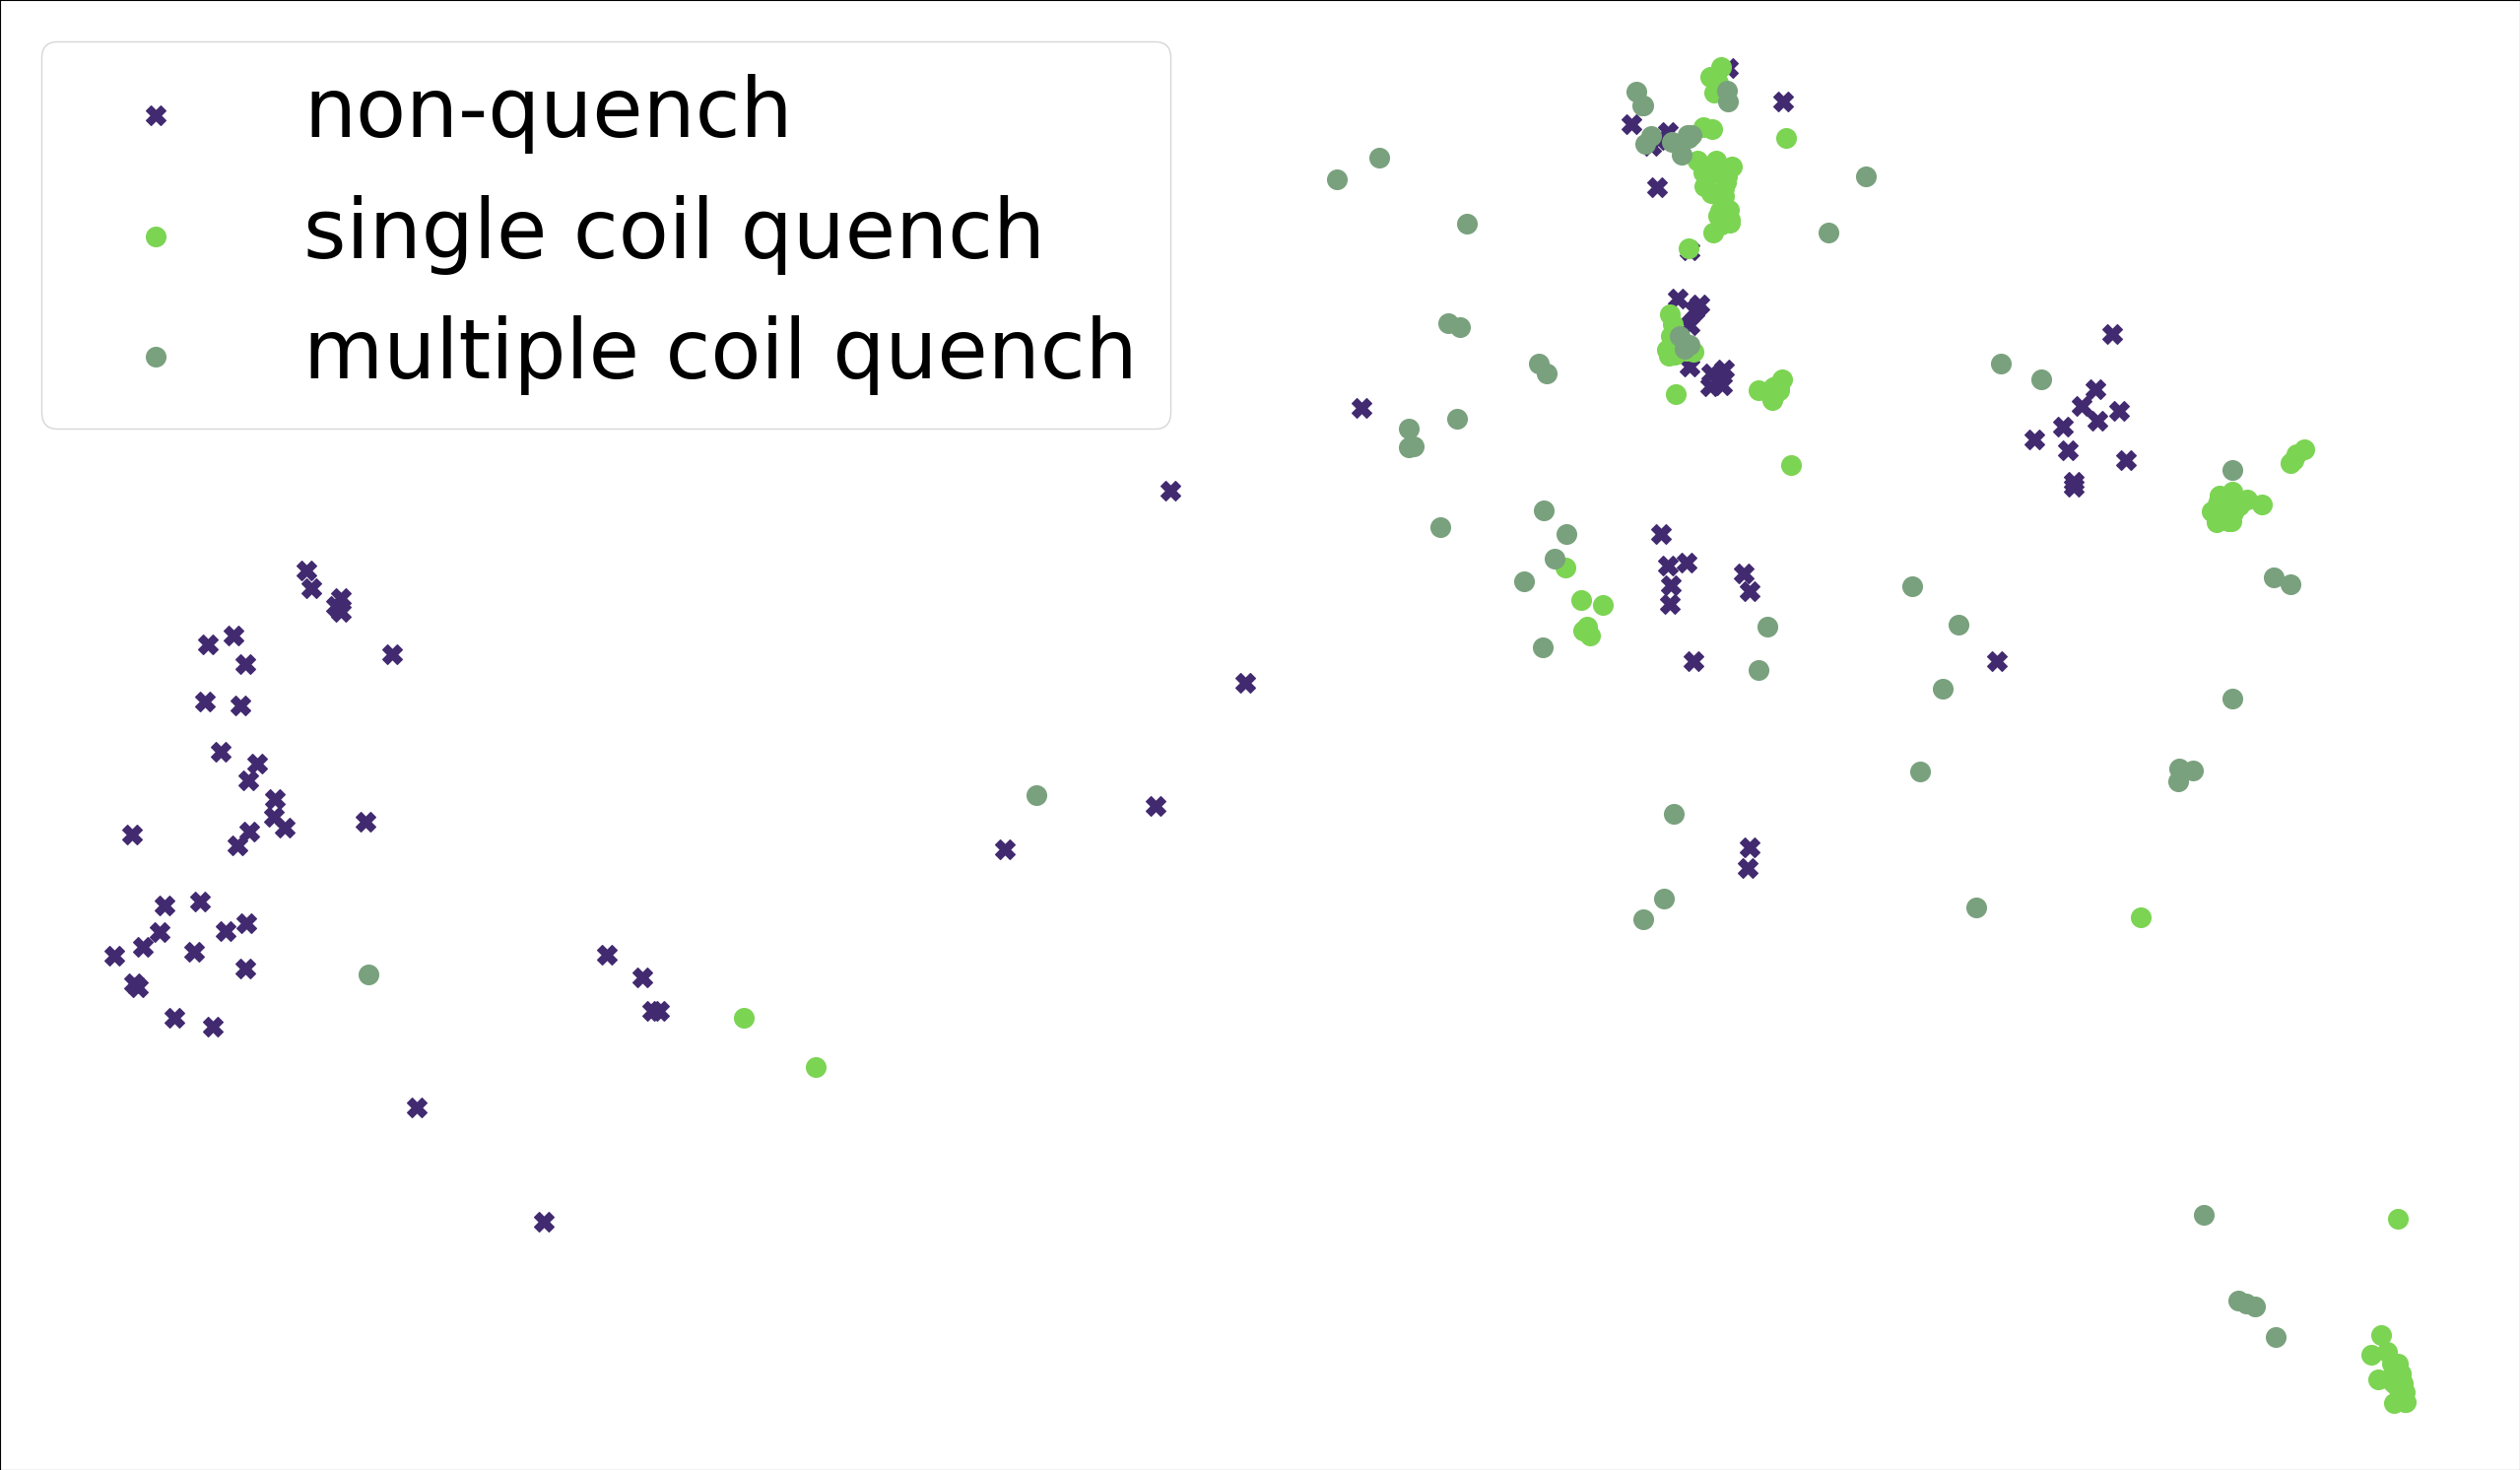
\includegraphics[width=\linewidth]{img/quench_dist_qlp/single_vs_multiple_Phi.png}
		\subcaption{}
	\end{subfigure}
	\begin{subfigure}{0.49\linewidth}
		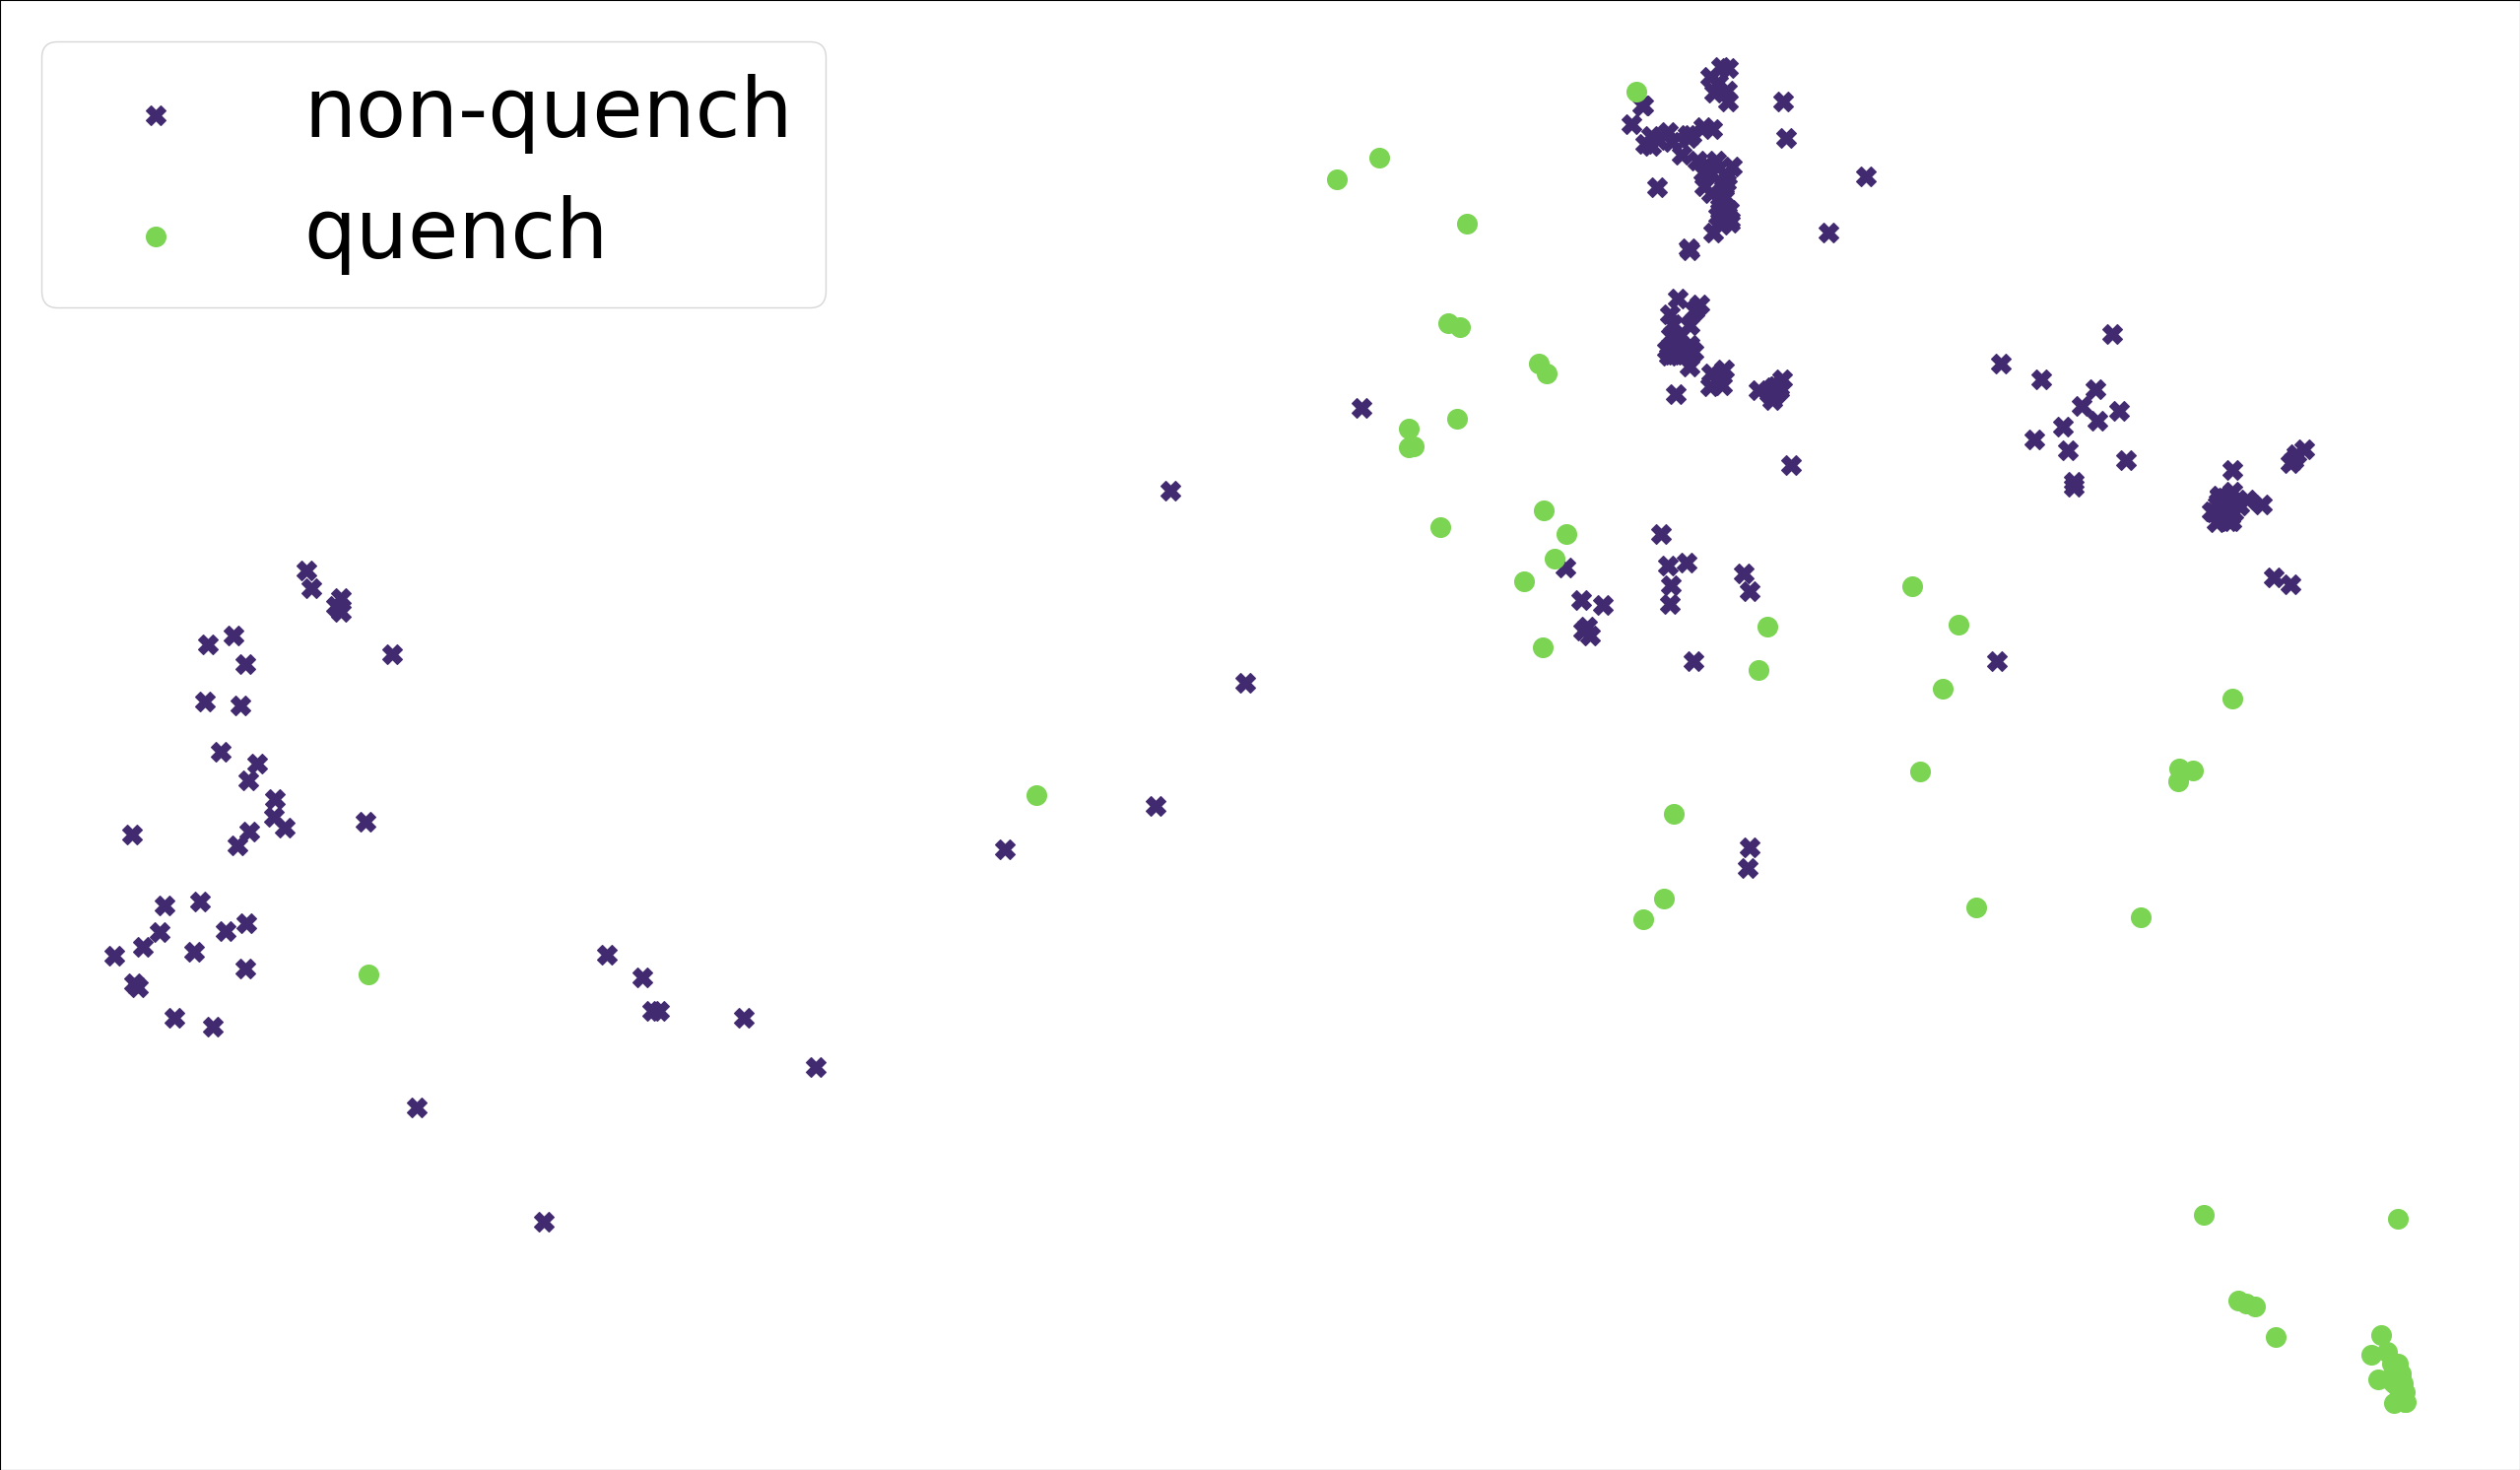
\includegraphics[width=\linewidth]{img/quench_dist_qlp/quenches_coil_0_Phi.png}
		\subcaption{}
	\end{subfigure}
	\begin{subfigure}{0.49\linewidth}
		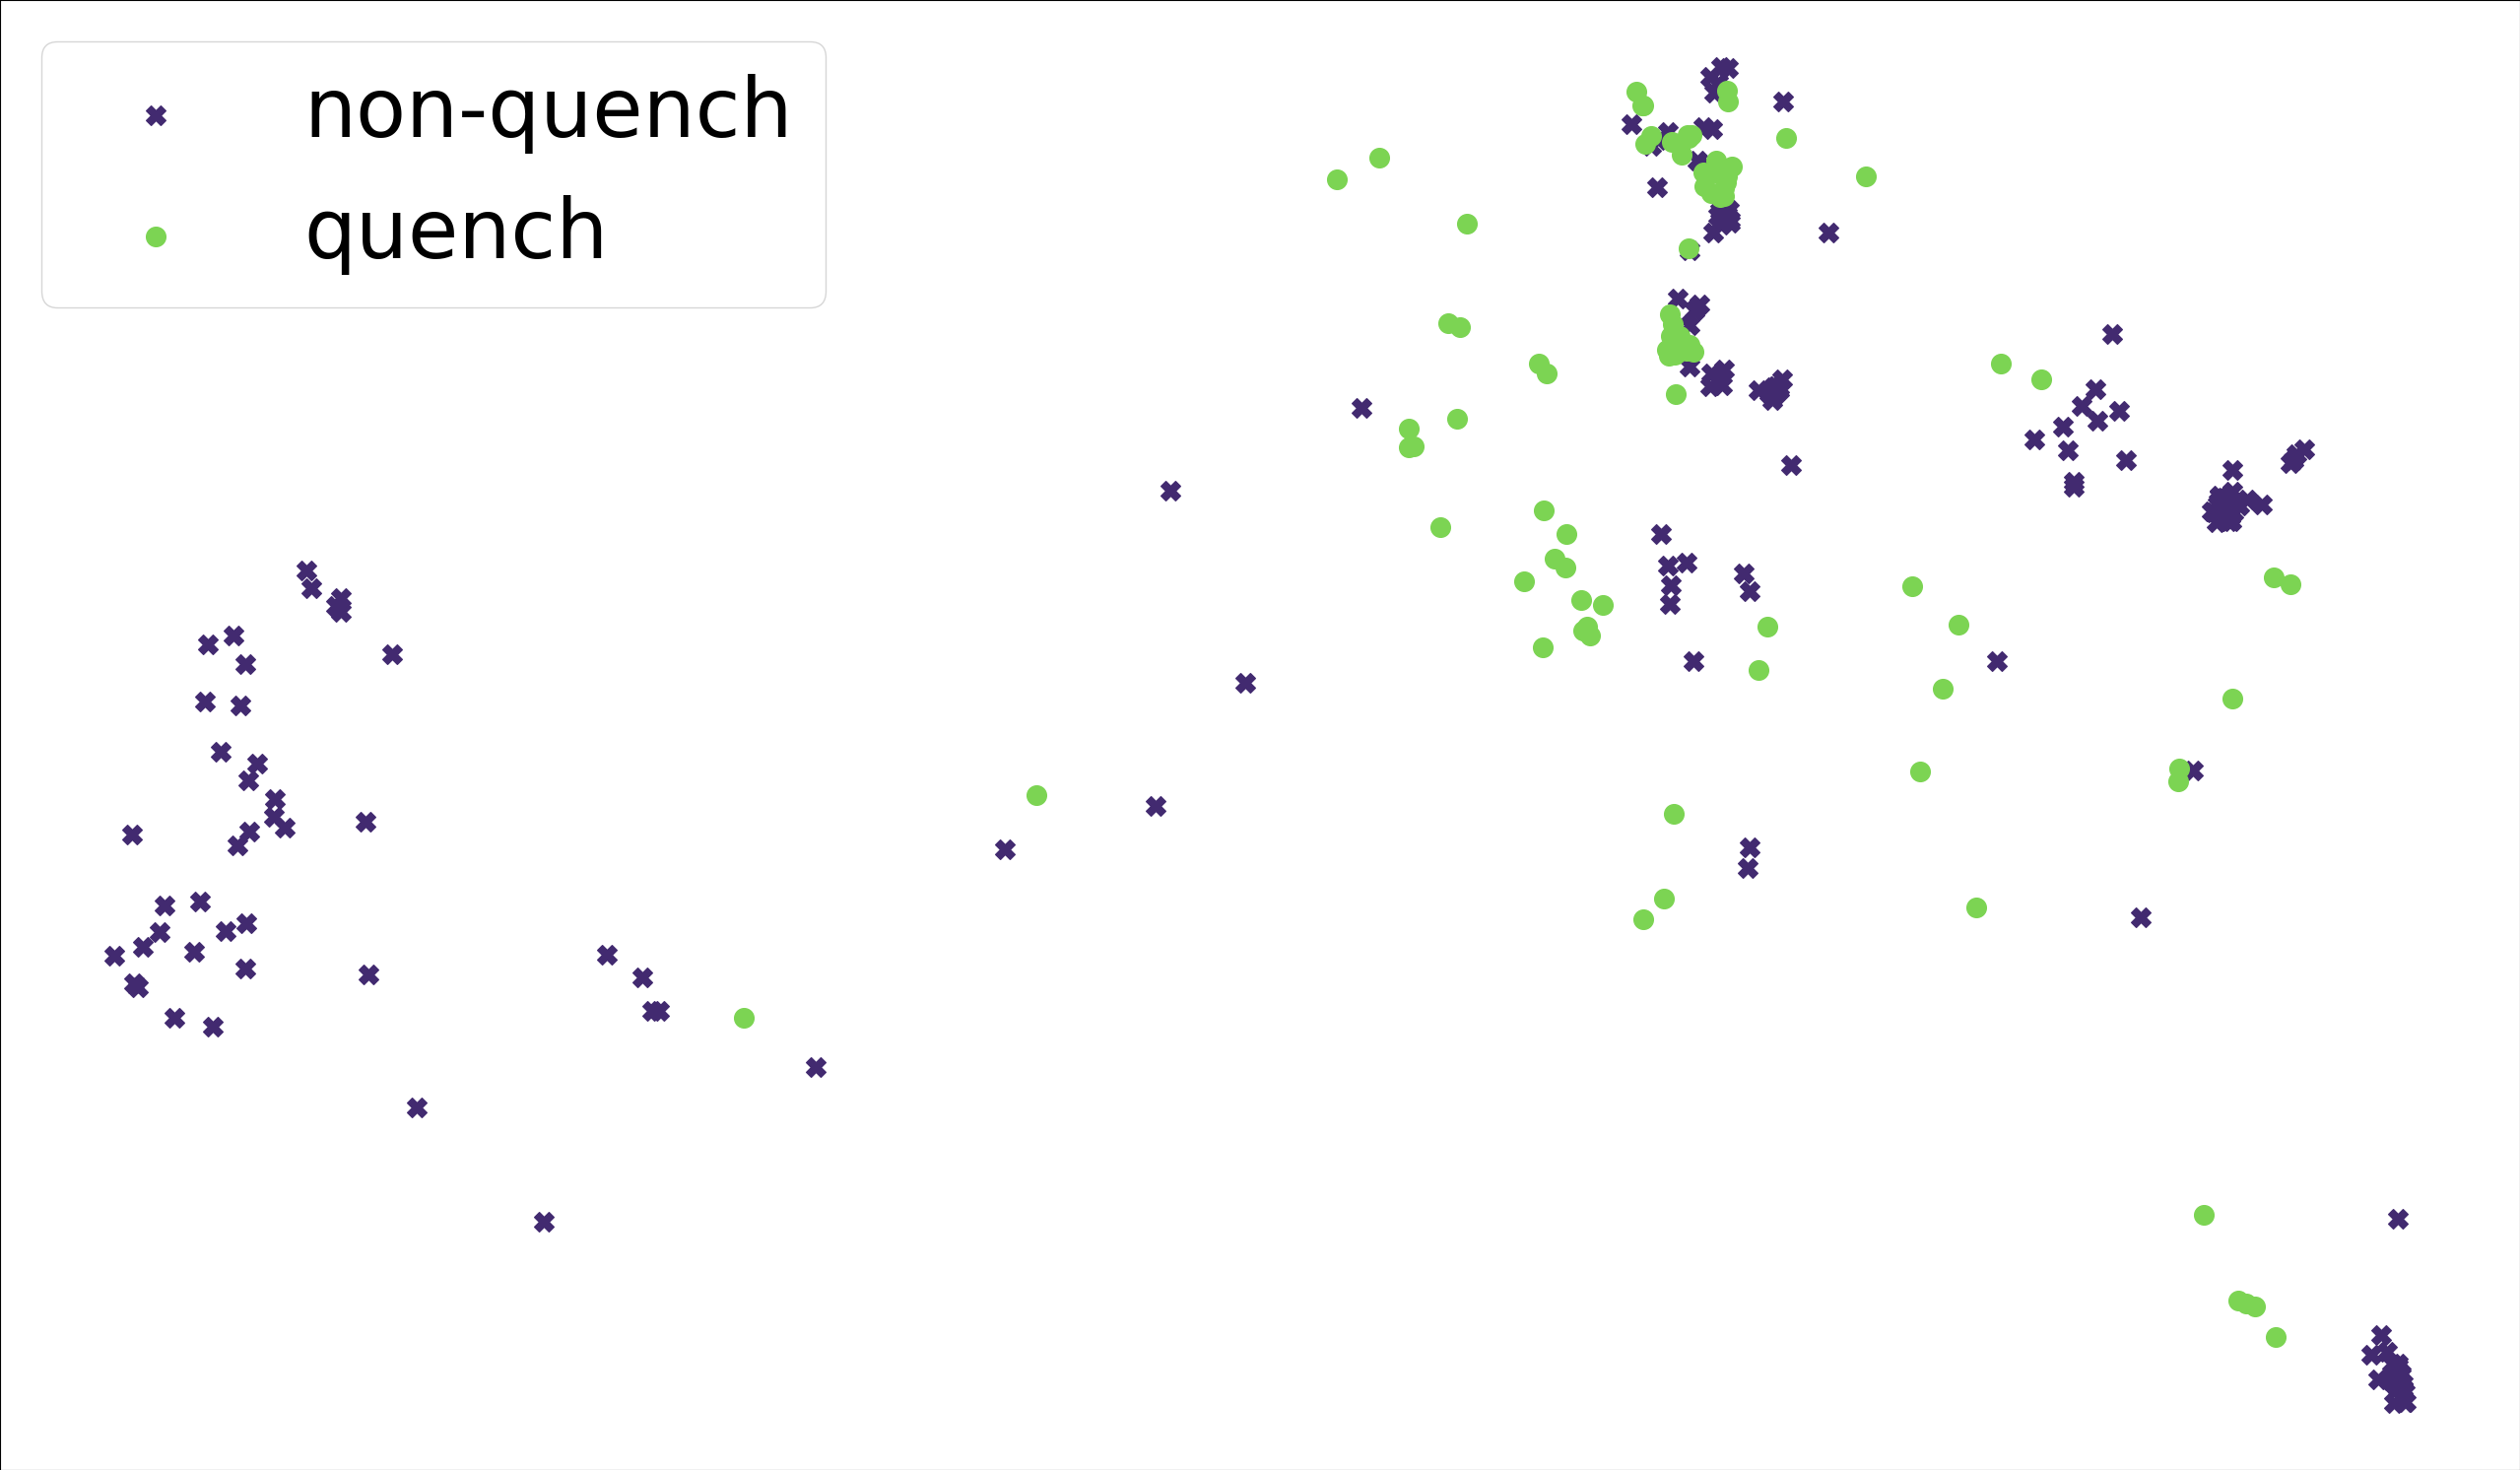
\includegraphics[width=\linewidth]{img/quench_dist_qlp/quenches_coil_1_Phi.png}
		\subcaption{}
	\end{subfigure}
	\begin{subfigure}{0.49\linewidth}
		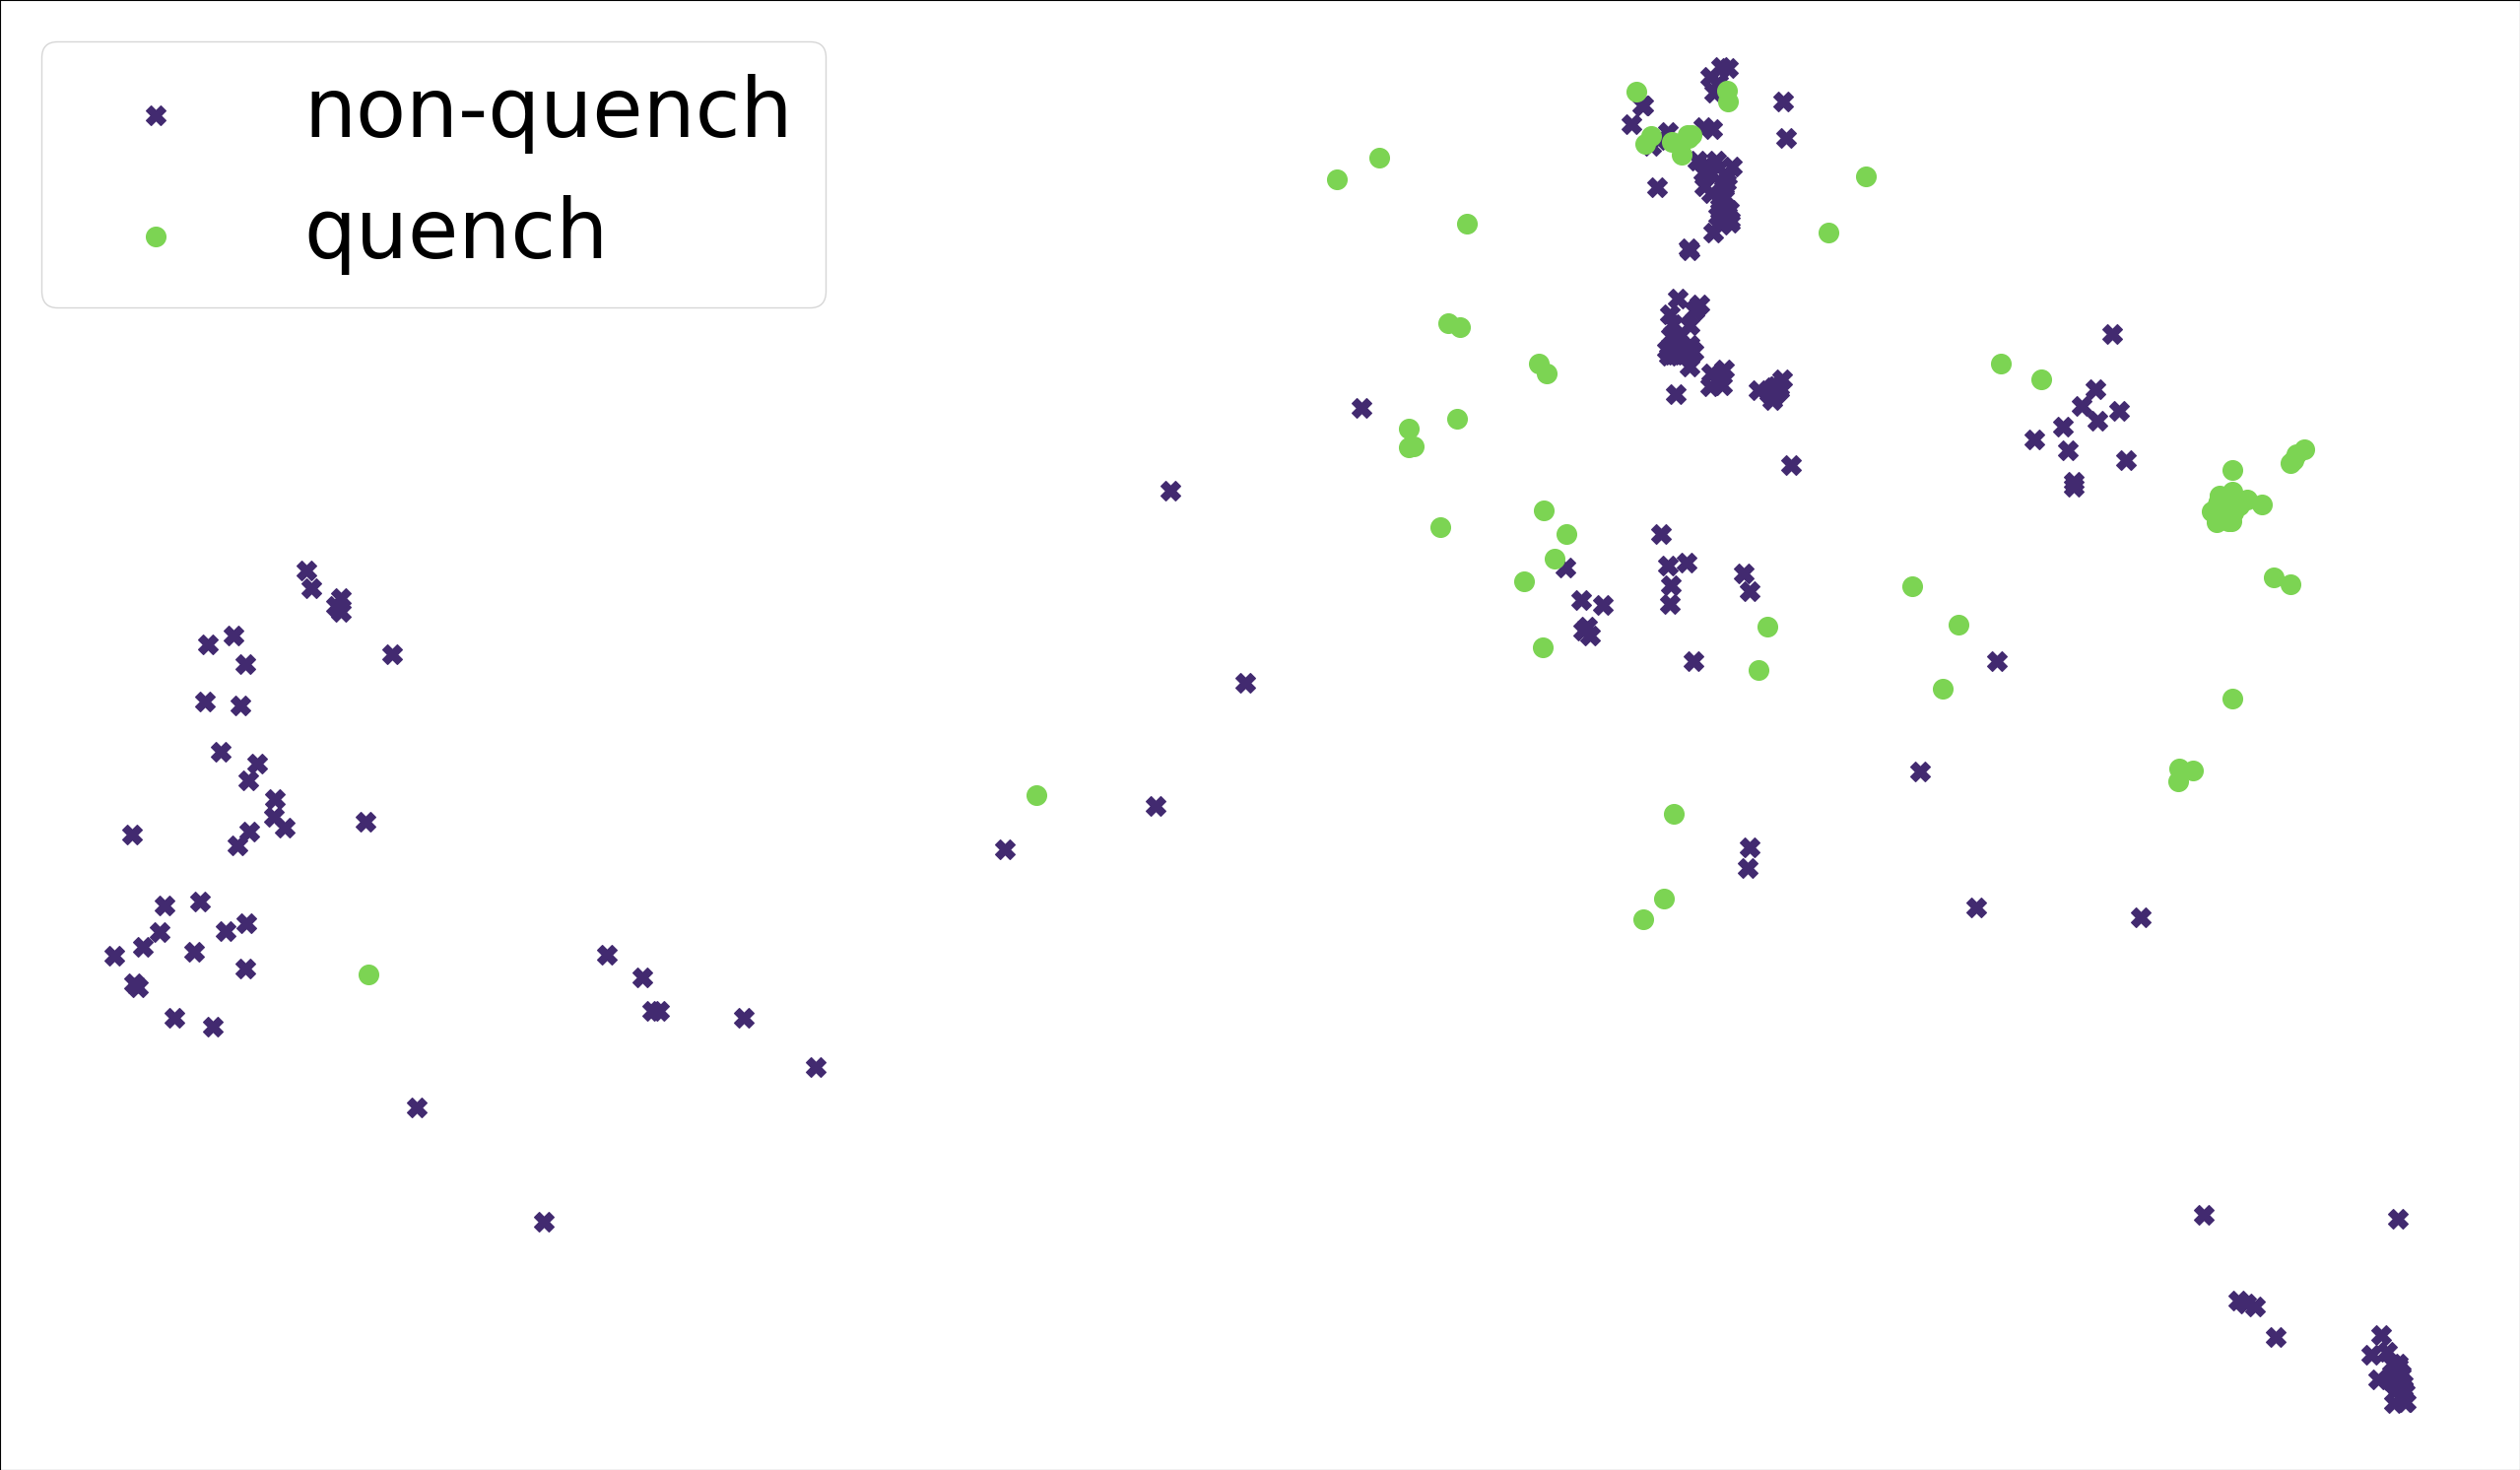
\includegraphics[width=\linewidth]{img/quench_dist_qlp/quenches_coil_2_Phi.png}
		\subcaption{}
	\end{subfigure}
	\begin{subfigure}{0.49\linewidth}
		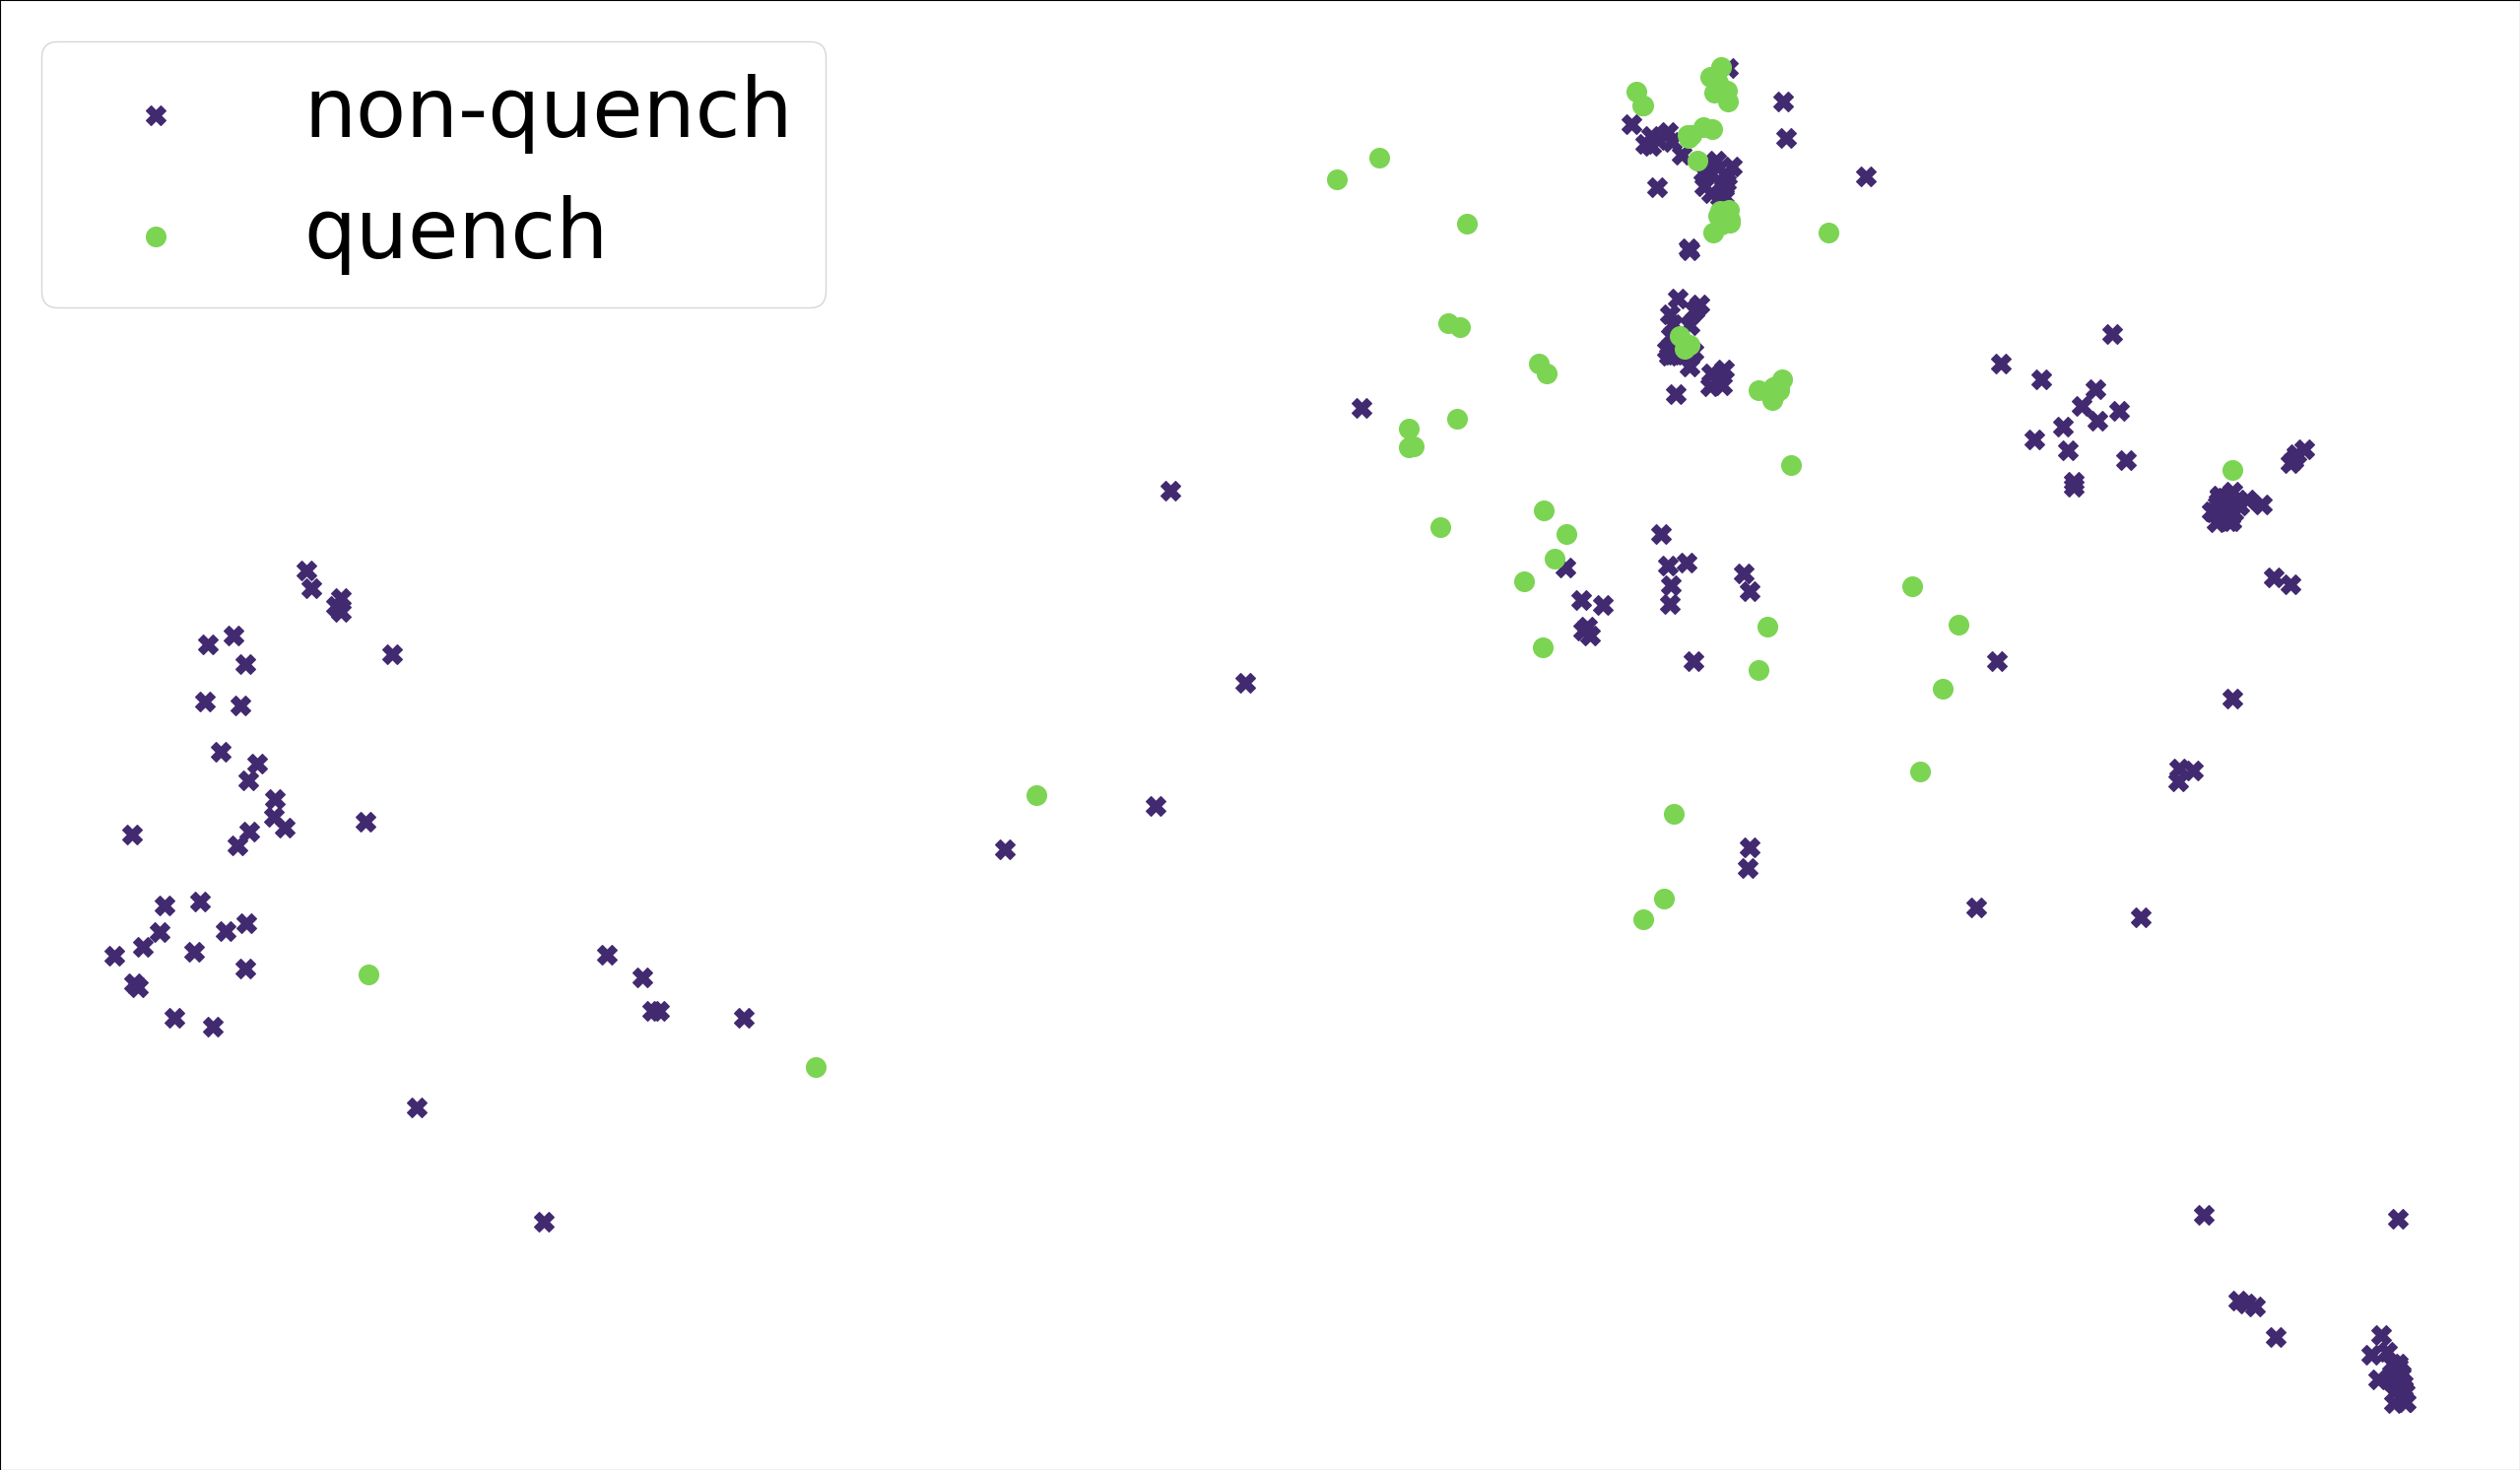
\includegraphics[width=\linewidth]{img/quench_dist_qlp/quenches_coil_3_Phi.png}
		\subcaption{}
	\end{subfigure}
	\caption{The distribution of the samples in bidimensional space after a round of \pca, for
		the \an\ attribute. the subfigures contain different views of the same data: (a) differenciates between non-quench and single or multiple quench events, (b) highlights the distribution of quenches for coil $0$, (c) highlights the distribution of quenches for coil $1$, (d) highlights the distribution of quenches for coil $2$ and finally (e) highlights the distribution of quenches for coil $3$.}
	\label{fig:phi-coilq-dist}
\end{figure}
\section{First approaches using Clustering}
\section{Extension of the QRP models}
\section{Results}
